%%____________________________________________________________________________||
\section{Results}
\label{sec:results}

The following section summarises the result of this analysis. The
control regions are populated with the full data set of 2016, namely
35.9\fbinv. As indicated in Sec.~\ref{sec:blinding}, the signal region
has been fully unblinded.

\subsection{Nominal result}
\label{sec:nominal-result}

Two different fits are performed. The {\it control-region-only fit} or
{\it masked fit} is constrained by data in the control regions only
and does not consider the observed data counts in the signal
region. The {\it signal-region fit} or {\it full fit} is constrained
by data counts in all control and signal regions, under the assumption
that no signal is present.  (Note that the terms {\it masked fit} and
{\it control-region-only fit} ({\it CR-only fit}) are also used
interchangeably.)

The result, in terms of observed data counts and the expected SM
contributions and uncertainties, are shown in Figs.~\ref{fig:no-fit},
\ref{fig:cr-fit}, and \ref{fig:full-fit}. (These figures supersede the
original presentation of the result, found in AN v4 and
Appendix~\ref{app:results-orig}.)

Figure~\ref{fig:no-fit} shows the results prior to fitting, so
contains just the observed data and predictions determined from
simulated event samples following (only) the application of the
corrections summarised in
Sec.~\ref{sec:sim-corrs}. Figures~\ref{fig:cr-fit} and
\ref{fig:full-fit} show the results of the control-region-only and
full fits, respectively.

For each fit, the results are divided into six subfigures, containing
the seven considered event topologies categorised according to \njet,
with the monojet and asymmetric events shown together. The different
\nb and \scalht categories are delineated by vertical lines, and the
\mht dimension is ``unrolled'' for each (\njet, \nb, \scalht)
category.

Each subfigure contains three panels.  The top panels show the event
yields in the signal region as observed in data (solid circles) and as
predicted in the SM (black histogram).  The uncertainties on the
prediction are indicated by the shaded bands, with the grey band for
the uncertainty on the total prediction and the burgundy shaded band
for the remnant multi-jet background. Central panels show the ratio of
the observed and expected counts.  Error bars contain both statistical
and systematic uncertainties and show the mid-P interval for the
ratio. Finally, the bottom panels provide the observed pull of the
data given by the difference between observed and expected yields and
normalised to the total uncertainty.  The total uncertainty is the
quadrature sum of the uncertainty on the prediction and the asymmetric
statistical uncertainty on the data. The upper (lower) value of the
statistical uncertainty on the data is used when the prediction is
above (below) the observed value.

%Each bin in figures~\ref{fig:no-fit}, \ref{fig:cr-fit}, and
%\ref{fig:full-fit} represents a different \HTmiss bin.  Bins are
%labelled for their \nj, \nb, and \scalht along the top of the plots,
%however, to improve readability, the \HTmiss value for the bin should
%be inferred from table~\ref{tab:SR_binning} in
%section~\ref{sec:binning-summary}.

Figure~\ref{fig:ratios_and_pulls} shows histograms of the masked fit
values of the data-to-background ratios and pulls for all event
categories (defined in terms of \njet, \nb, and \scalht, yet inclusive
with respect to \mht). Figure~\ref{fig:pulls} shows the pulls as a
function of (\njet, \nb) event category and \scalht, with counts
integrated over \mht, obtained from the masked fit.
%A goodness-of-fit estimate can be obtained by considering the pulls
%obtained from the masked fit, which in the following are assumed to be
%derived from independent background estimates. The summation over the
%squares of the pulls from 101 (\njet, \nb, \scalht) categories,
%summarised in Fig.~\ref{fig:pulls}, gives a $\chi^2$ value of
%73.0. Hence the reduced $\chi^2$ and the p-value are 0.72 and 0.98,
%respectively.

Figure~\ref{fig:breakdown} provides the breakdown of SM backgrounds
(categorised as lost lepton, \znunuj, or multijet) in the signal
region as determined from the CR-only and full fits.

Appendices~\ref{app:results-tables-pre},
\ref{app:results-tables-cronly}, and \ref{app:results-tables-full}
contain tables presenting the data counts and background expectations
in the signal (and, for the first, \mj and \mmj control regions) for
the pre-, CR-only-, and full-fit results, respectively. 

Finally, App.~\ref{app:nuispost} contains figures showing the post-fit
behaviour of the nuisance parameters relative to their pre-fit values.

\clearpage
\begin{figure}[!h]
  \centering
  \subfigure[\label{fig:no-fit:mono-asymm}Monojet and asymmetric topologies]{
    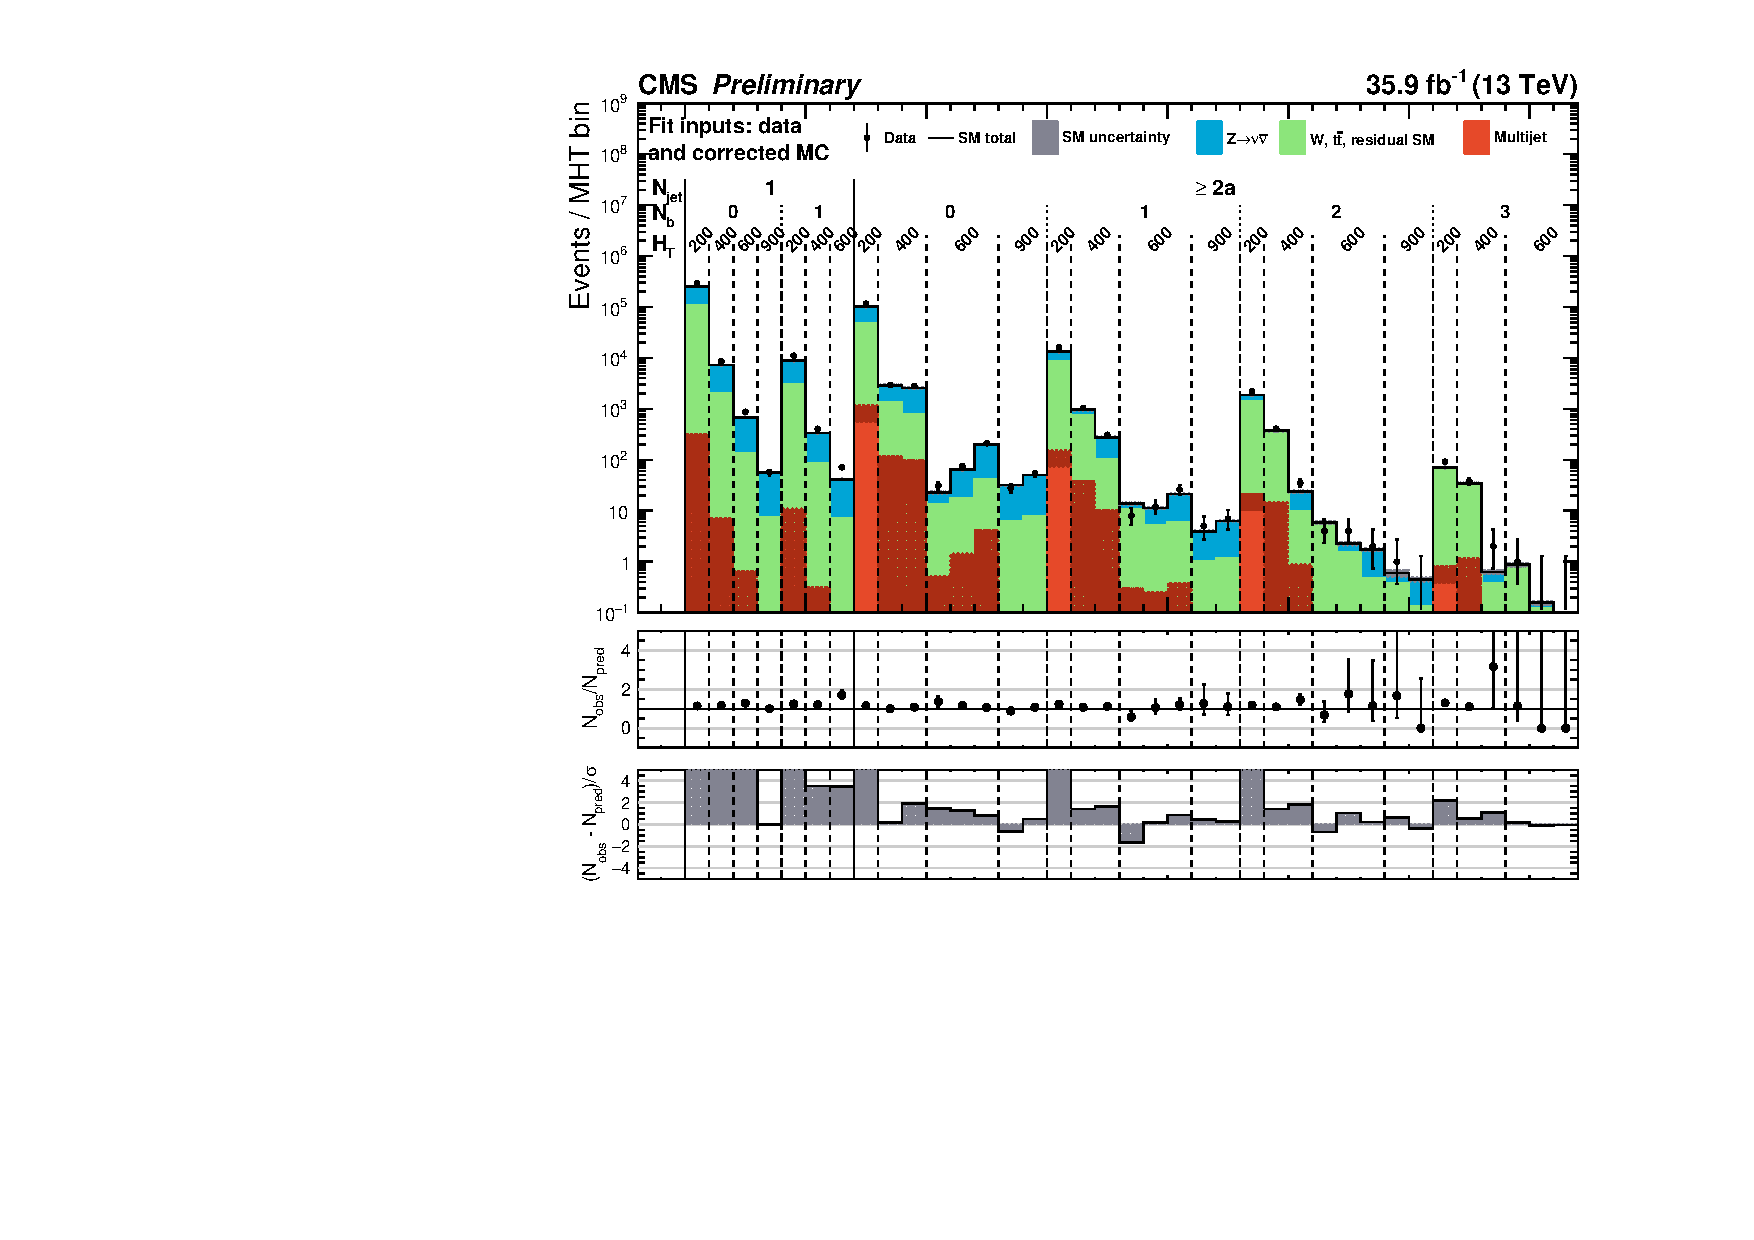
\includegraphics[width=0.48\textwidth]{figures/results/36invfb_preapproval/mht_binned/no-fit/monojet_no-fit.pdf}
  }~ 
  \subfigure[\label{fig:no-fit:dijet}Dijet topologies]{
    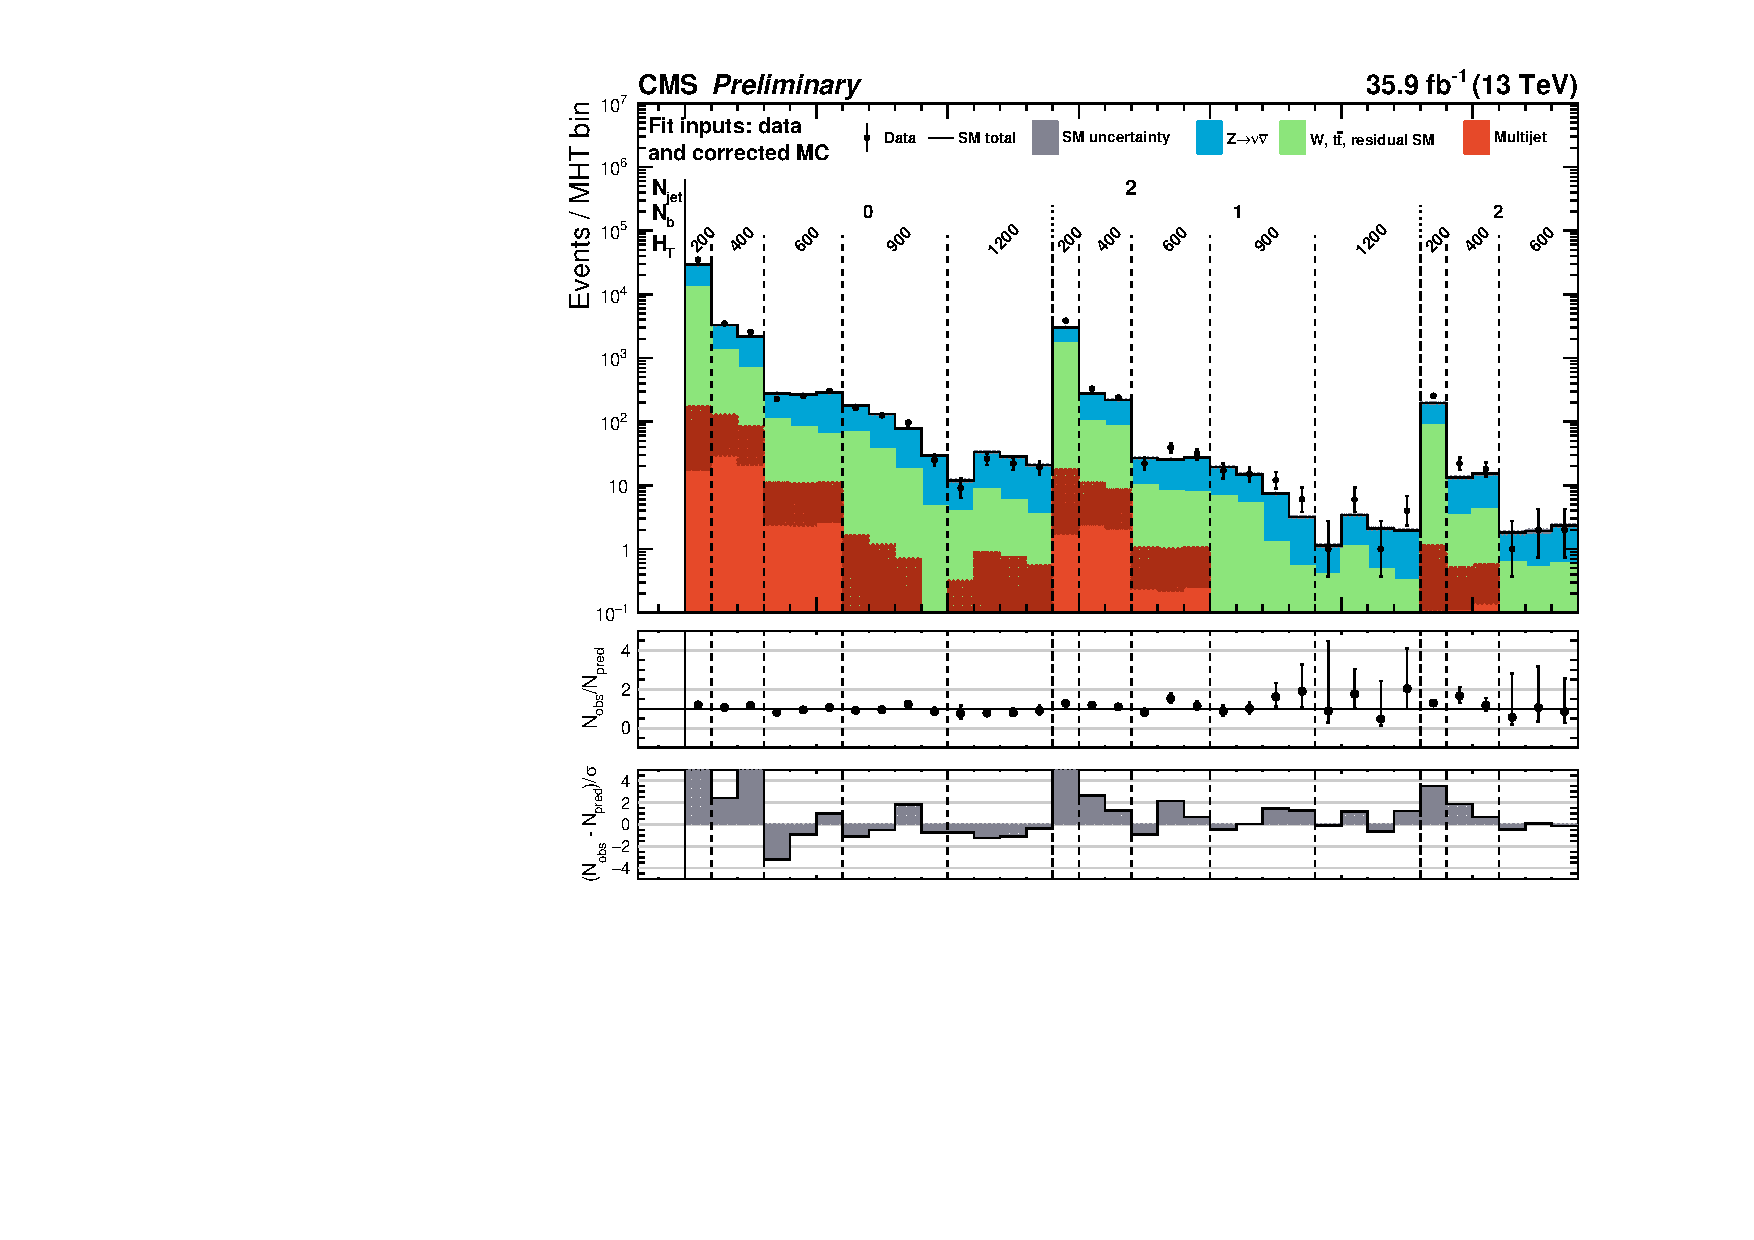
\includegraphics[width=0.48\textwidth]{figures/results/36invfb_preapproval/mht_binned/no-fit/di-jet_no-fit.pdf}
  }\\
  \subfigure[\label{fig:no-fit:three-jet}Topologies with 3 jets]{
    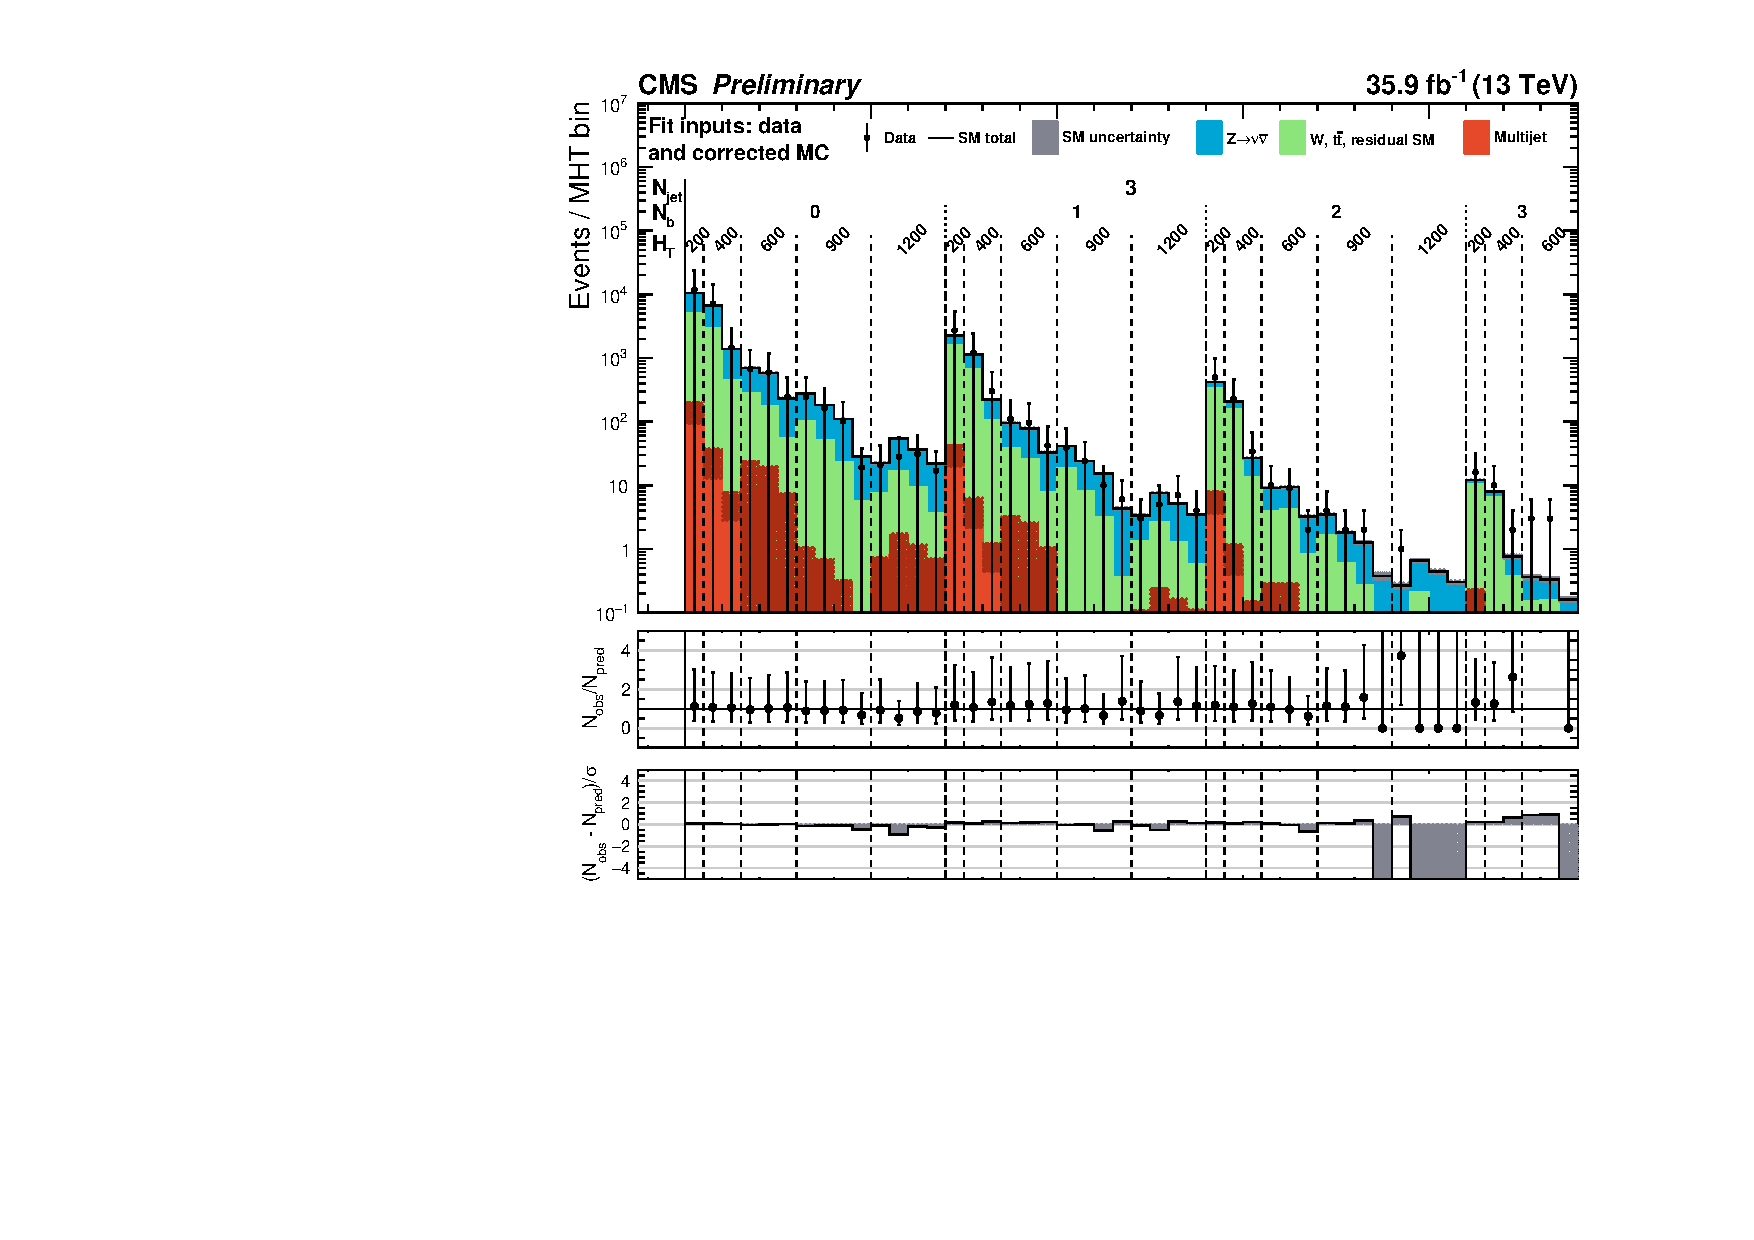
\includegraphics[width=0.48\textwidth]{figures/results/36invfb_preapproval/mht_binned/no-fit/3jet_no-fit.pdf}
  }~ 
  \subfigure[\label{fig:no-fit:four-jet}Topologies with 4 jets]{
    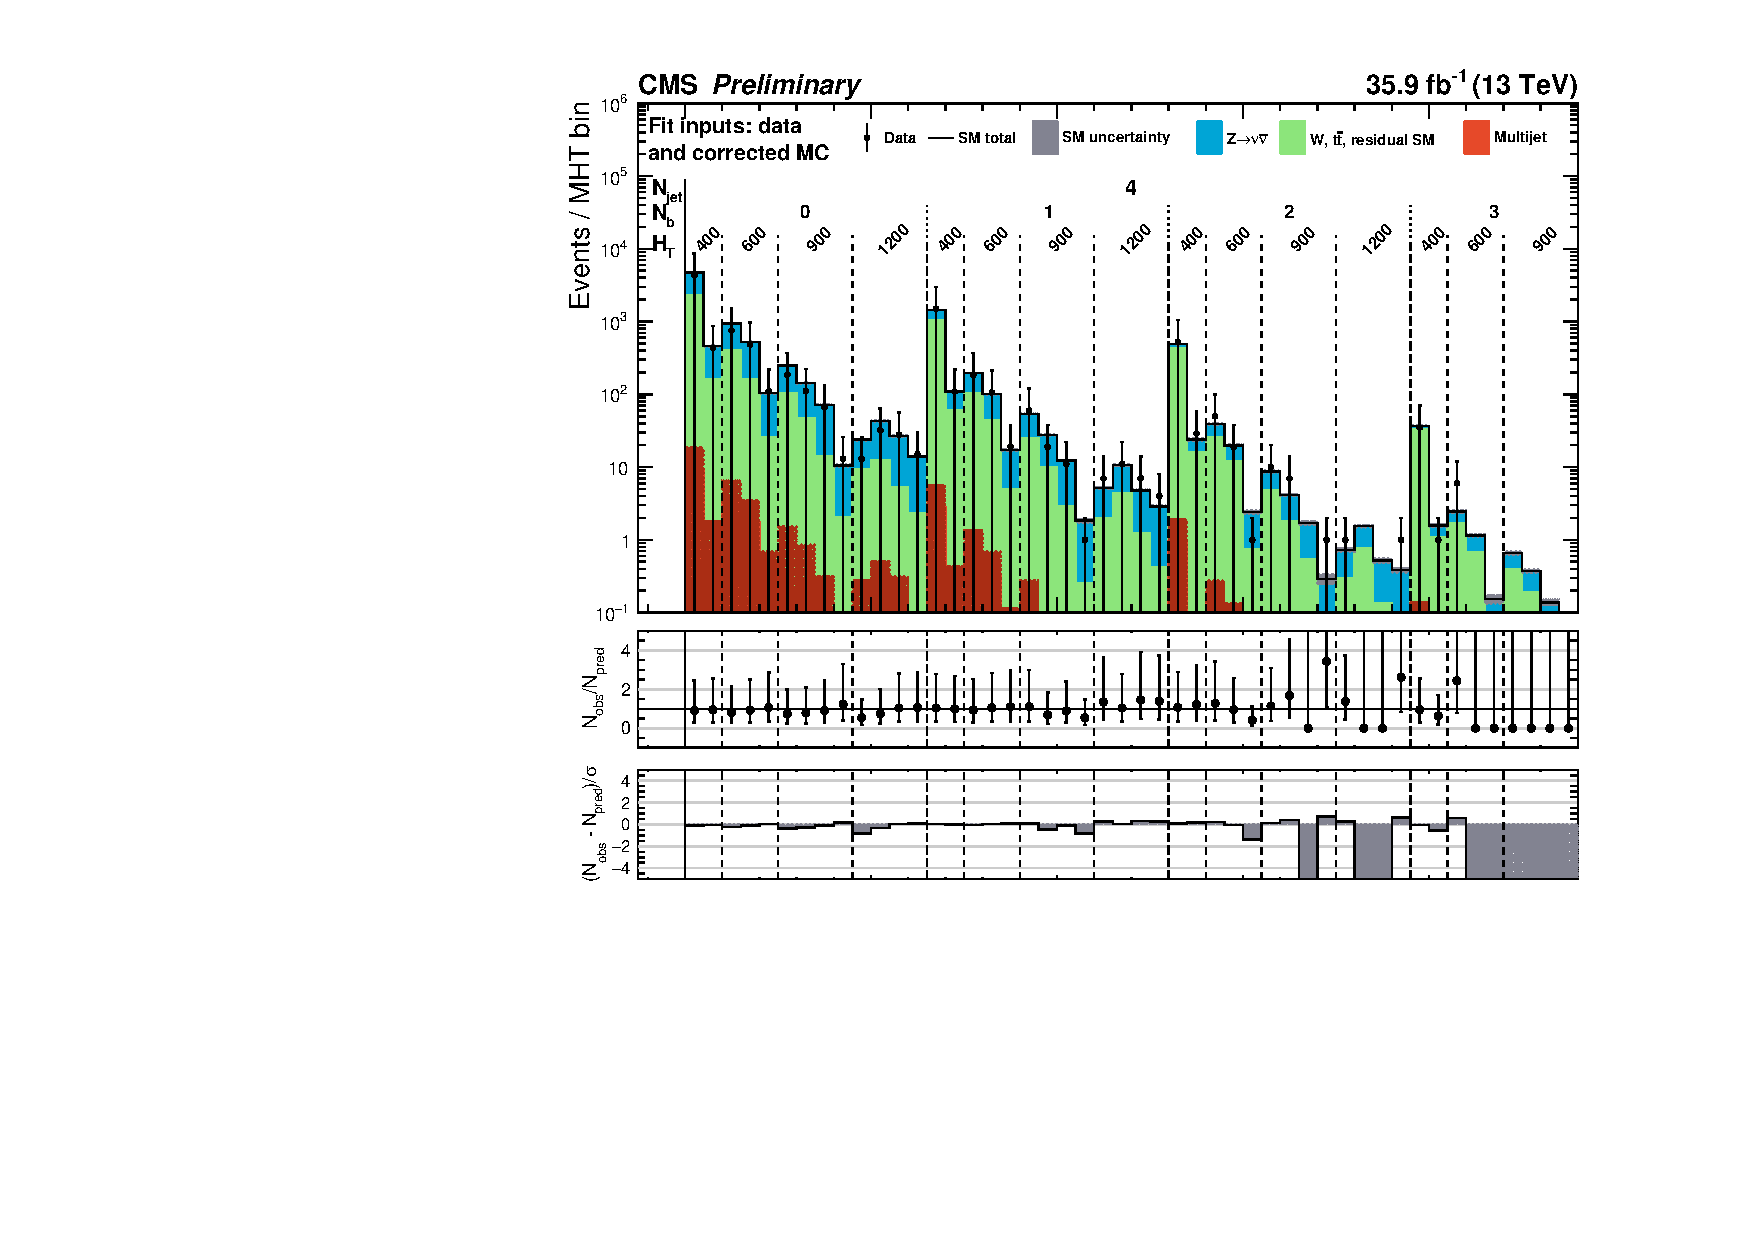
\includegraphics[width=0.48\textwidth]{figures/results/36invfb_preapproval/mht_binned/no-fit/4jet_no-fit.pdf}
  }\\
  \subfigure[\label{fig:no-fit:five-jet}Topologies with 5 jets]{
    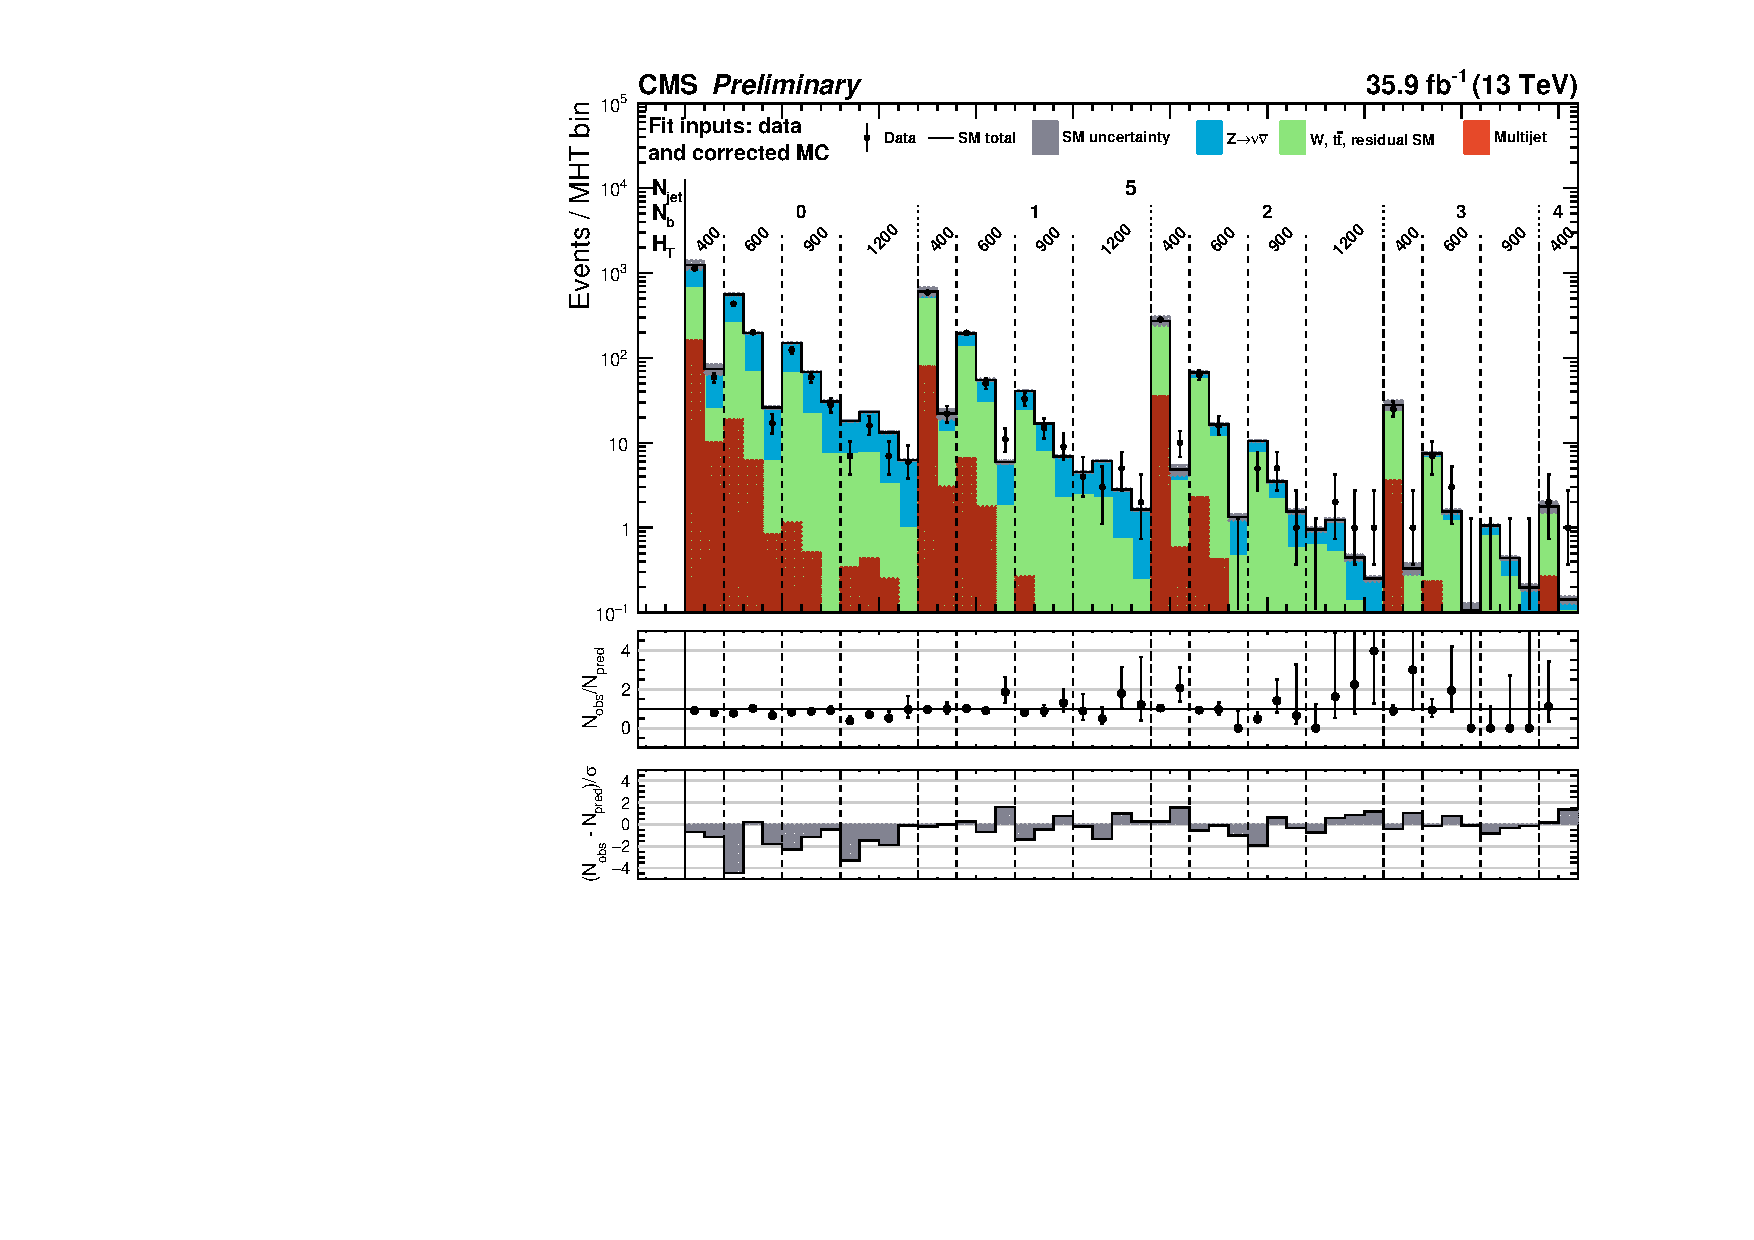
\includegraphics[width=0.48\textwidth]{figures/results/36invfb_preapproval/mht_binned/no-fit/5jet_no-fit.pdf}
  }~ 
  \subfigure[\label{fig:no-fit:six-jet}Topologies with $\ge$6 jets]{
    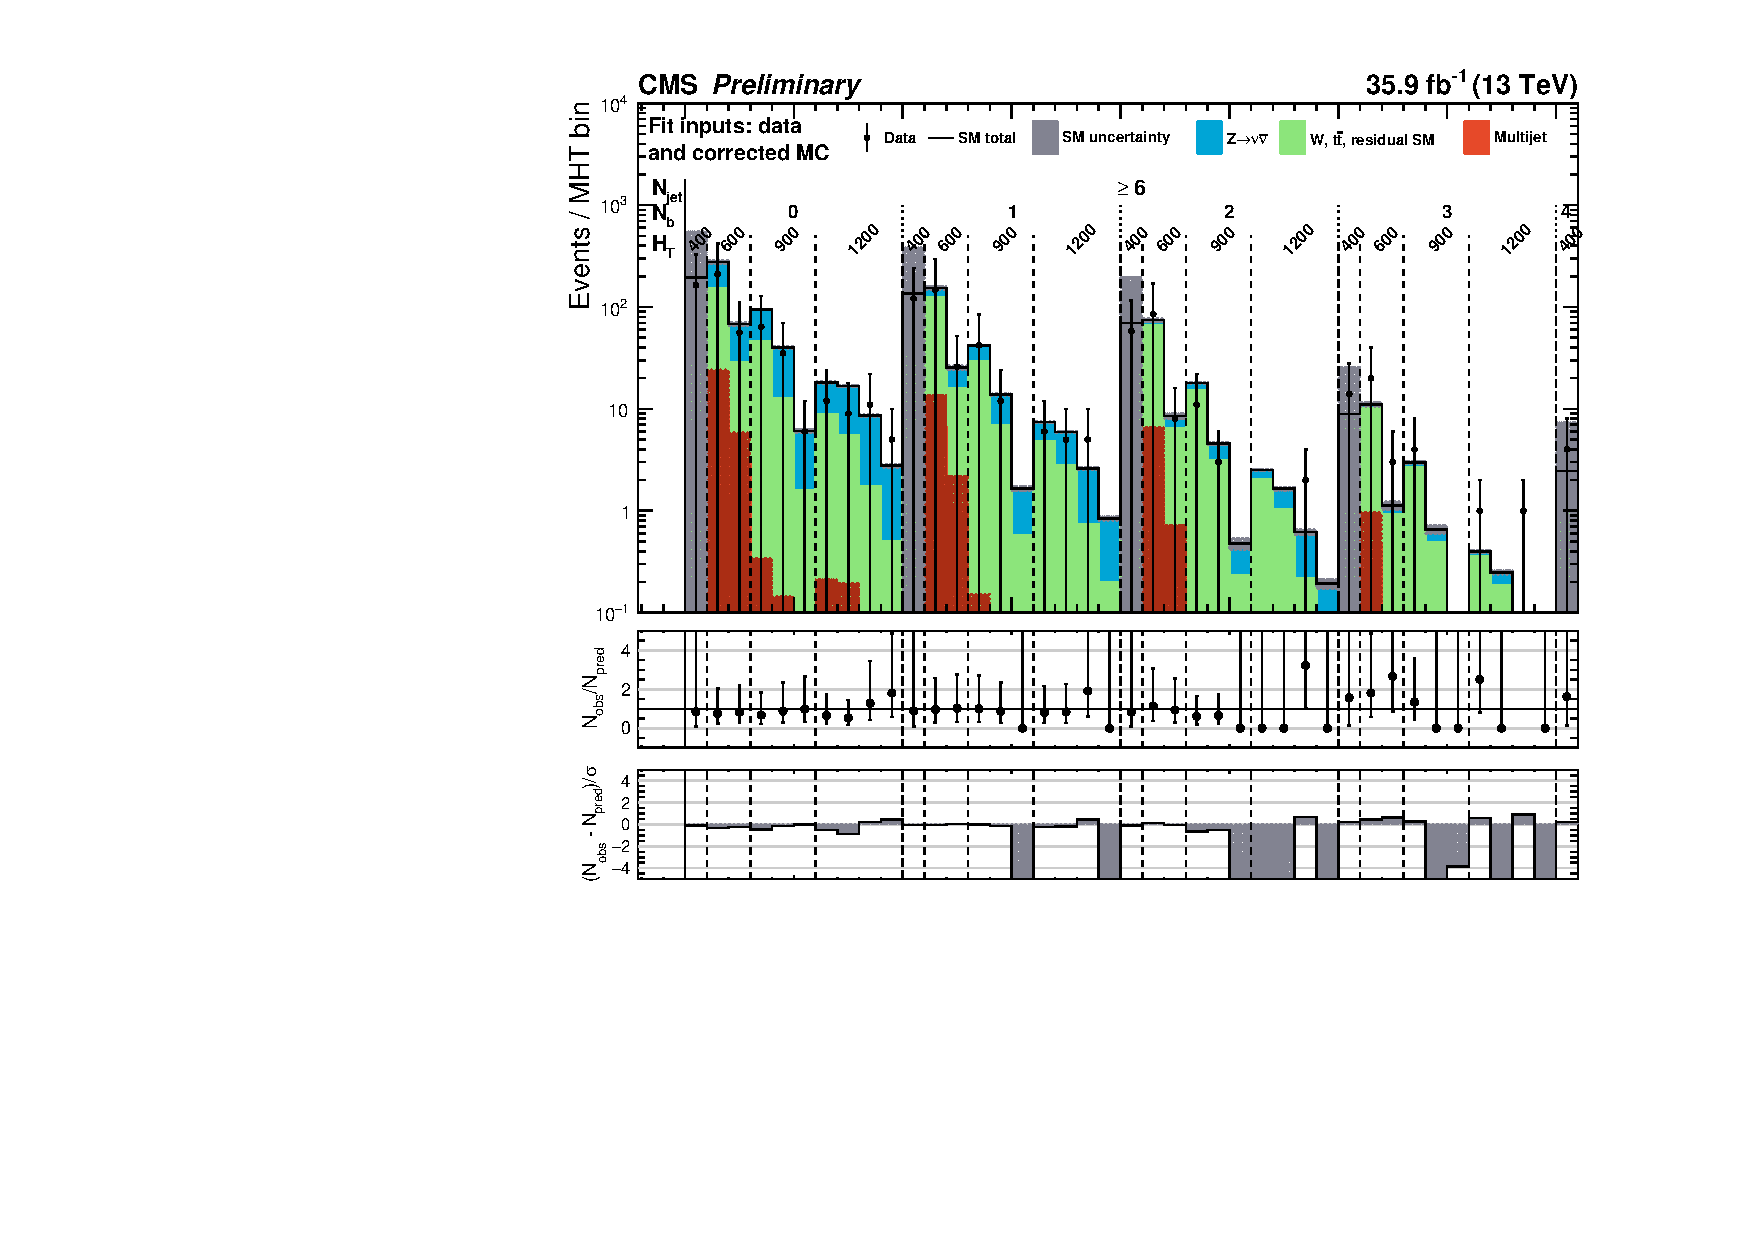
\includegraphics[width=0.48\textwidth]{figures/results/36invfb_preapproval/mht_binned/no-fit/6+_jets_no-fit.pdf}
  }\\
  \caption{\label{fig:no-fit} Corrected MC predictions and data before fitting.
  Top panels:  Event yields in data and SM expectations.
  Centre panels:  Ratio of the observed and expected counts.
  Bottom panels:  Observed pulls of the data from expectation.
  Detailed descriptions are given in the text.
	}
\end{figure}

\clearpage
\begin{figure}[!h]
  \centering
  \subfigure[\label{fig:cr-fit:mono-asymm}Monojet and asymmetric topologies]{
    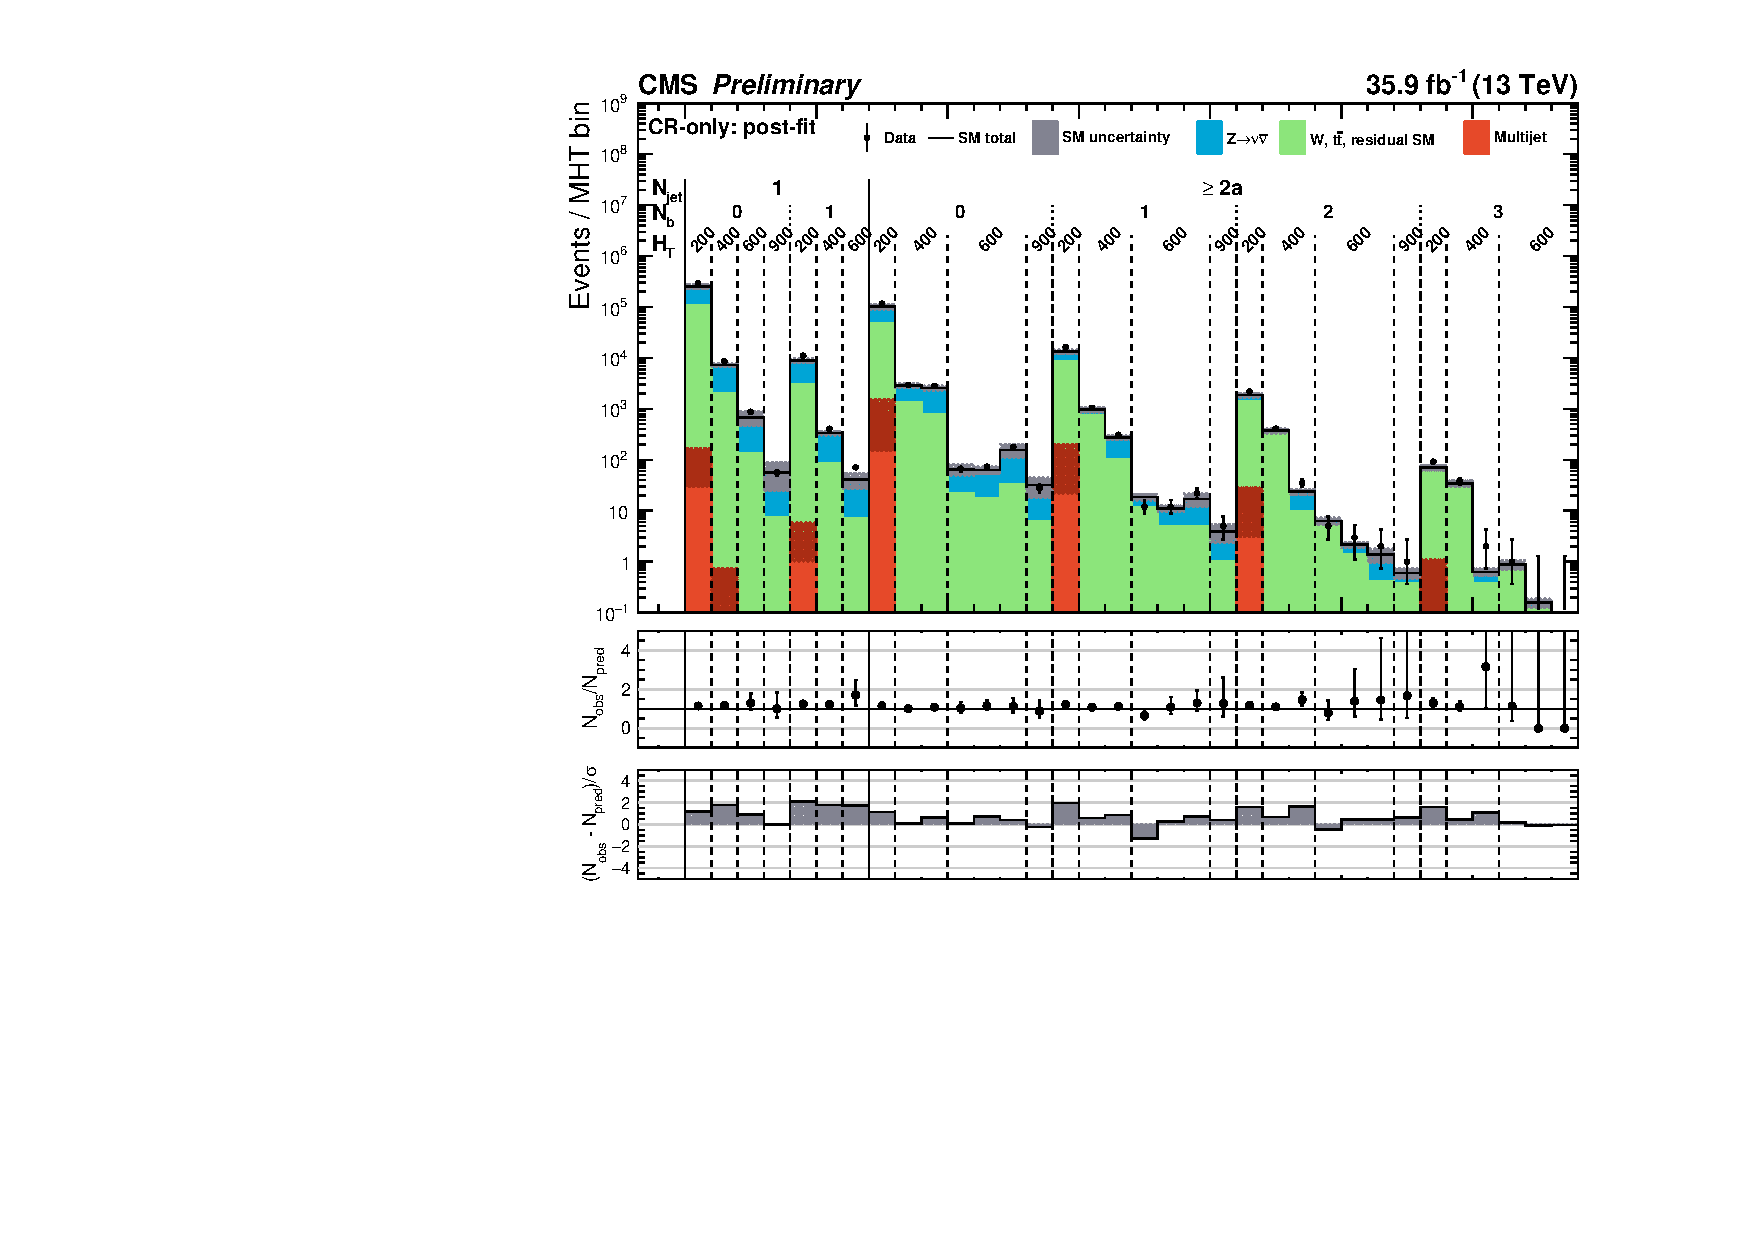
\includegraphics[width=0.48\textwidth]{figures/results/36invfb_preapproval/mht_binned/cr-only/monojet_cr-only.pdf}
  }~ 
  \subfigure[\label{fig:cr-fit:dijet}Dijet topologies]{
    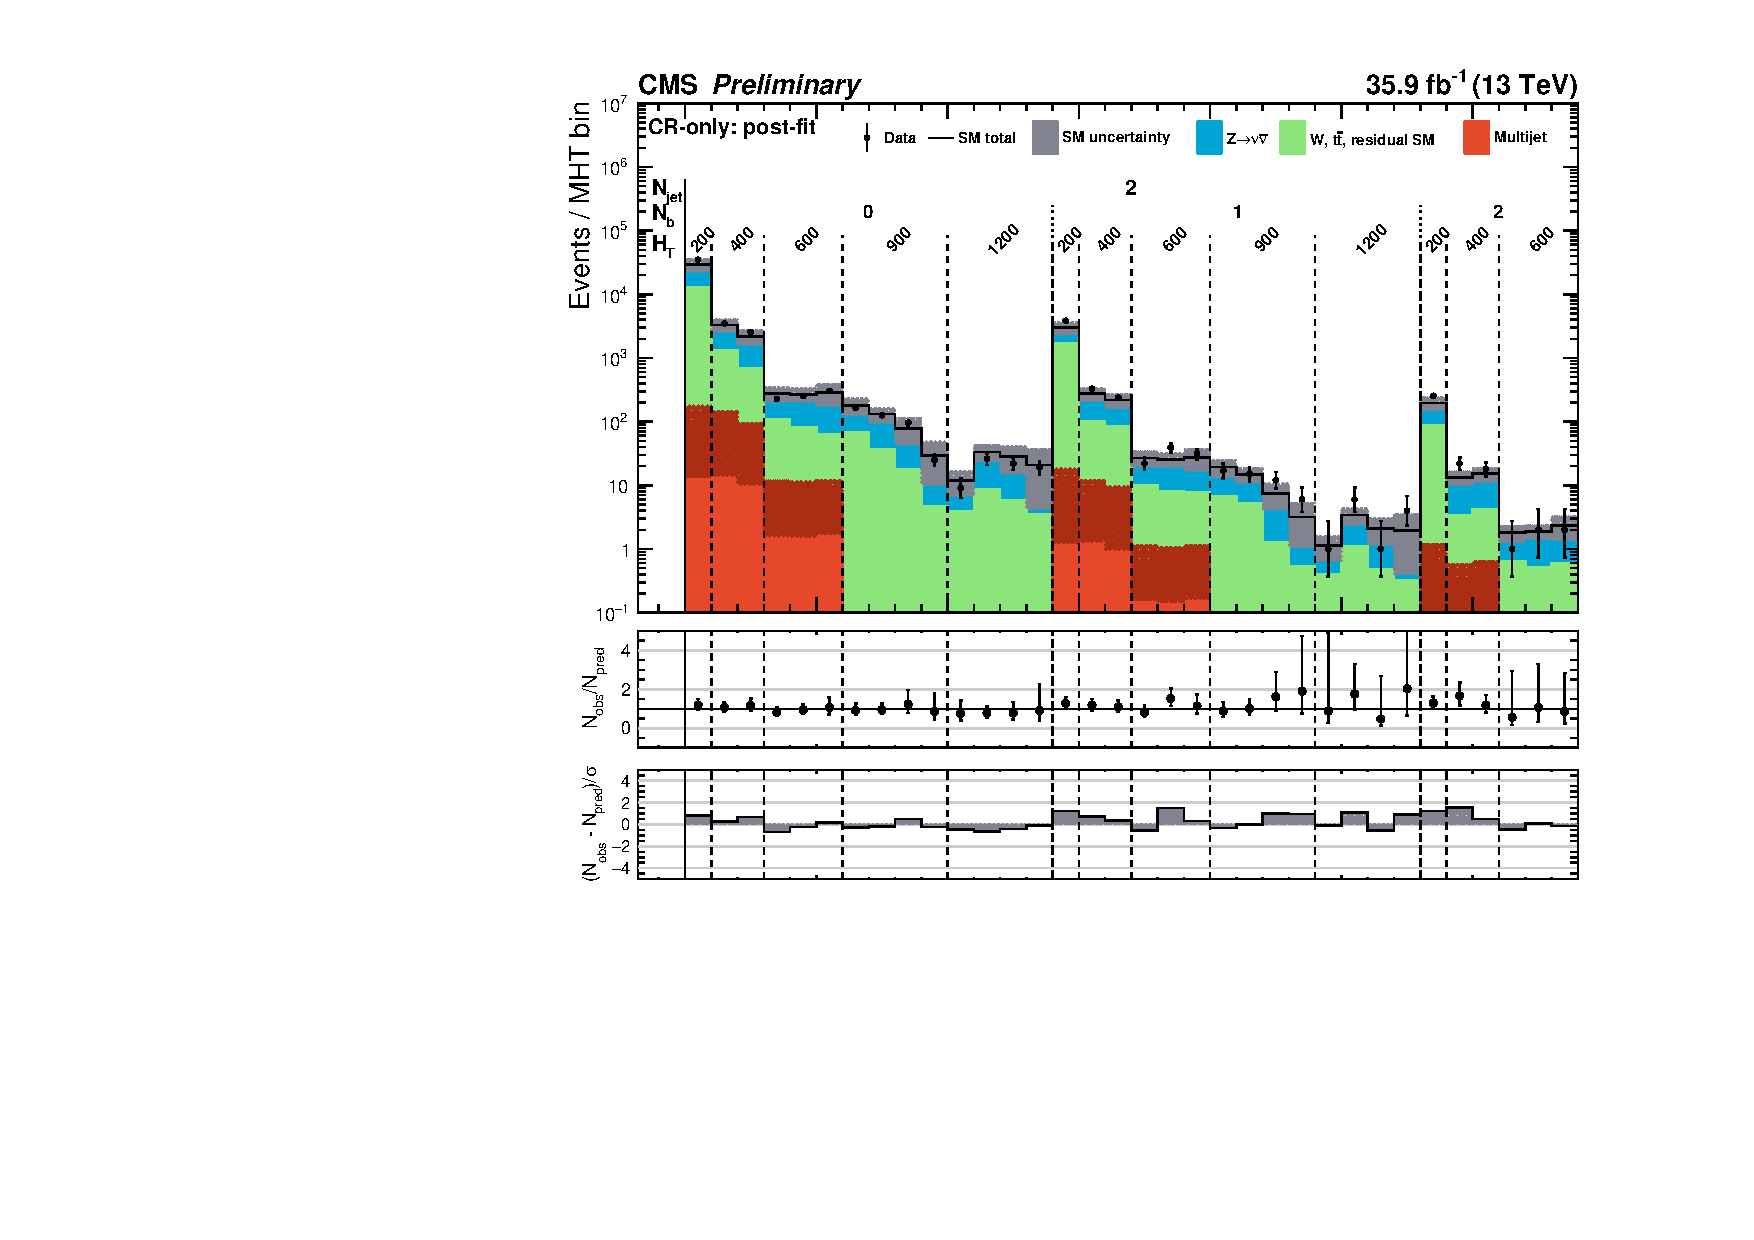
\includegraphics[width=0.48\textwidth]{figures/results/36invfb_preapproval/mht_binned/cr-only/di-jet_cr-only.pdf}
  }\\
  \subfigure[\label{fig:cr-fit:three-jet}Topologies with 3 jets]{
    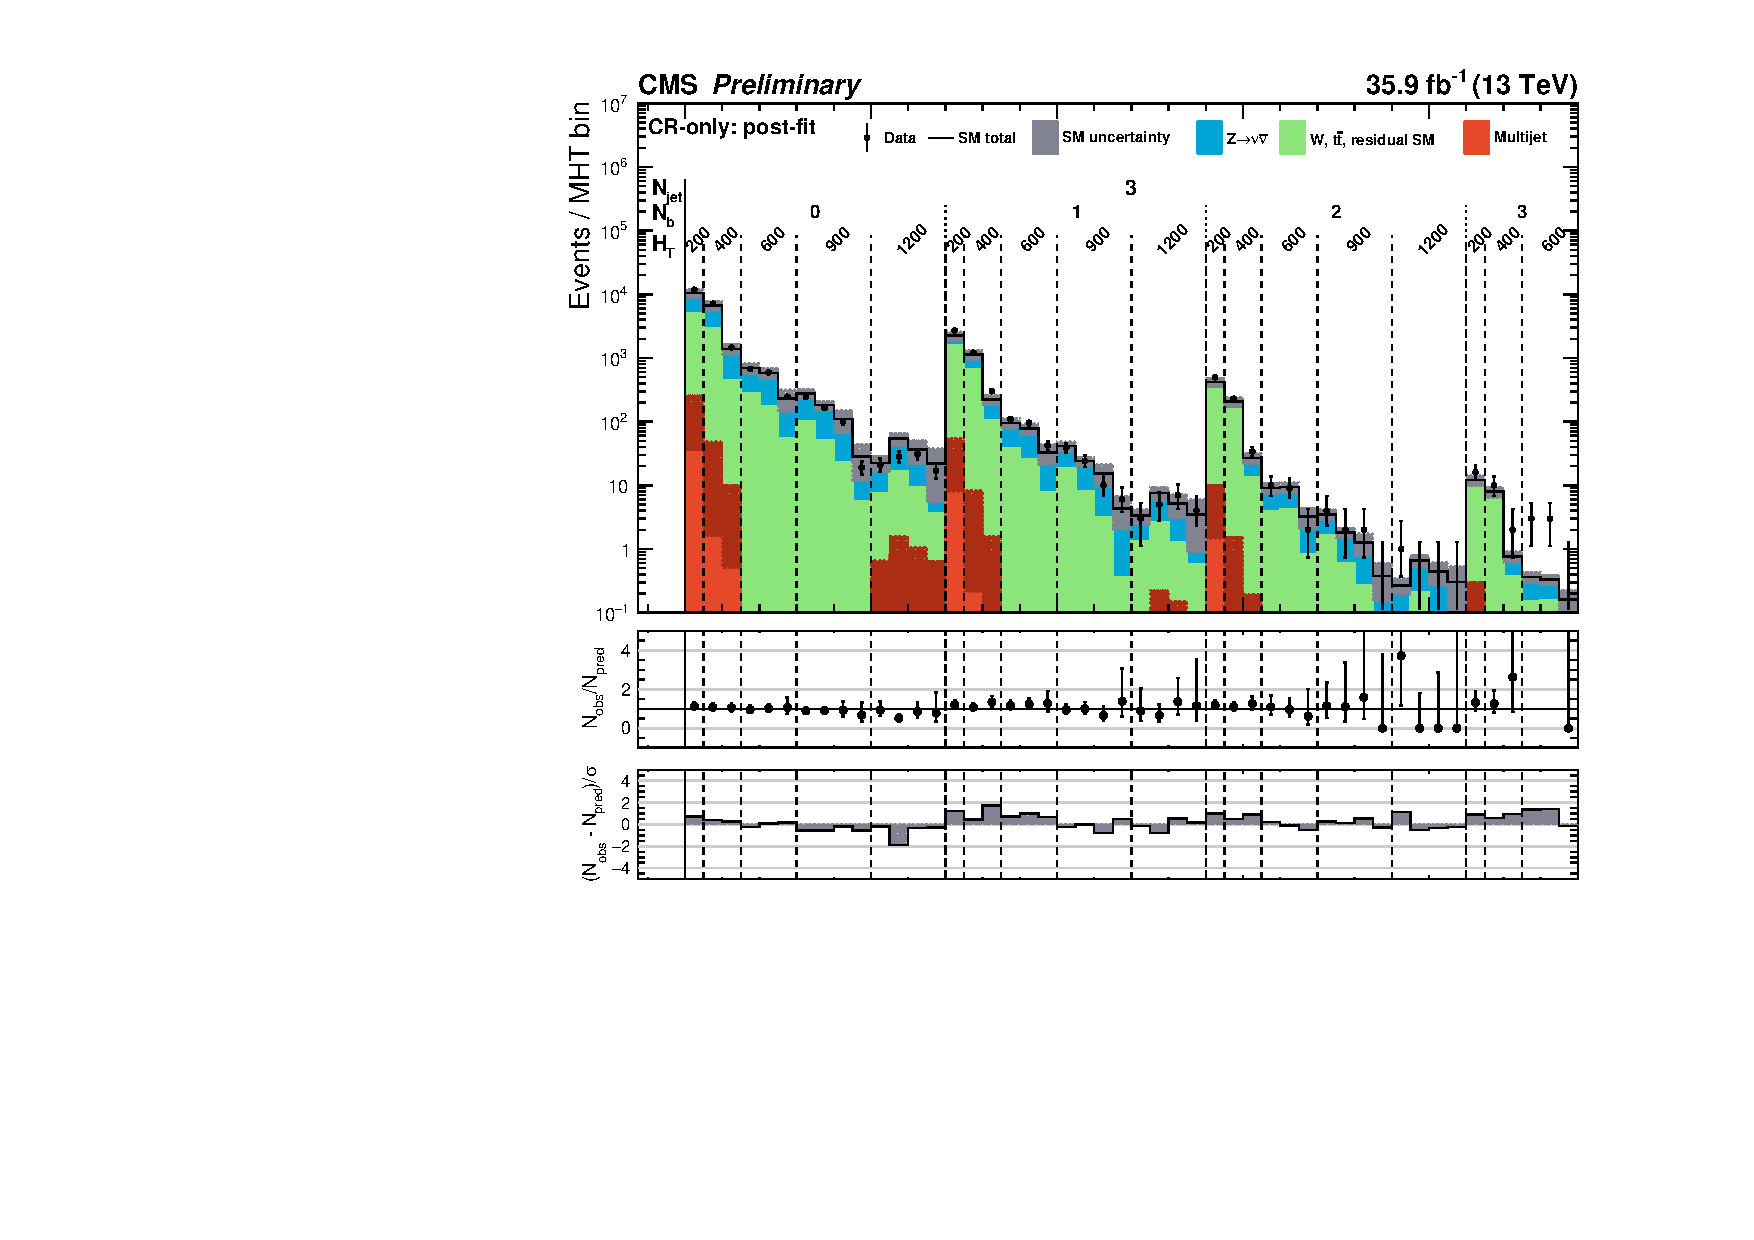
\includegraphics[width=0.48\textwidth]{figures/results/36invfb_preapproval/mht_binned/cr-only/3jet_cr-only.pdf}
  }~ 
  \subfigure[\label{fig:cr-fit:four-jet}Topologies with 4 jets]{
    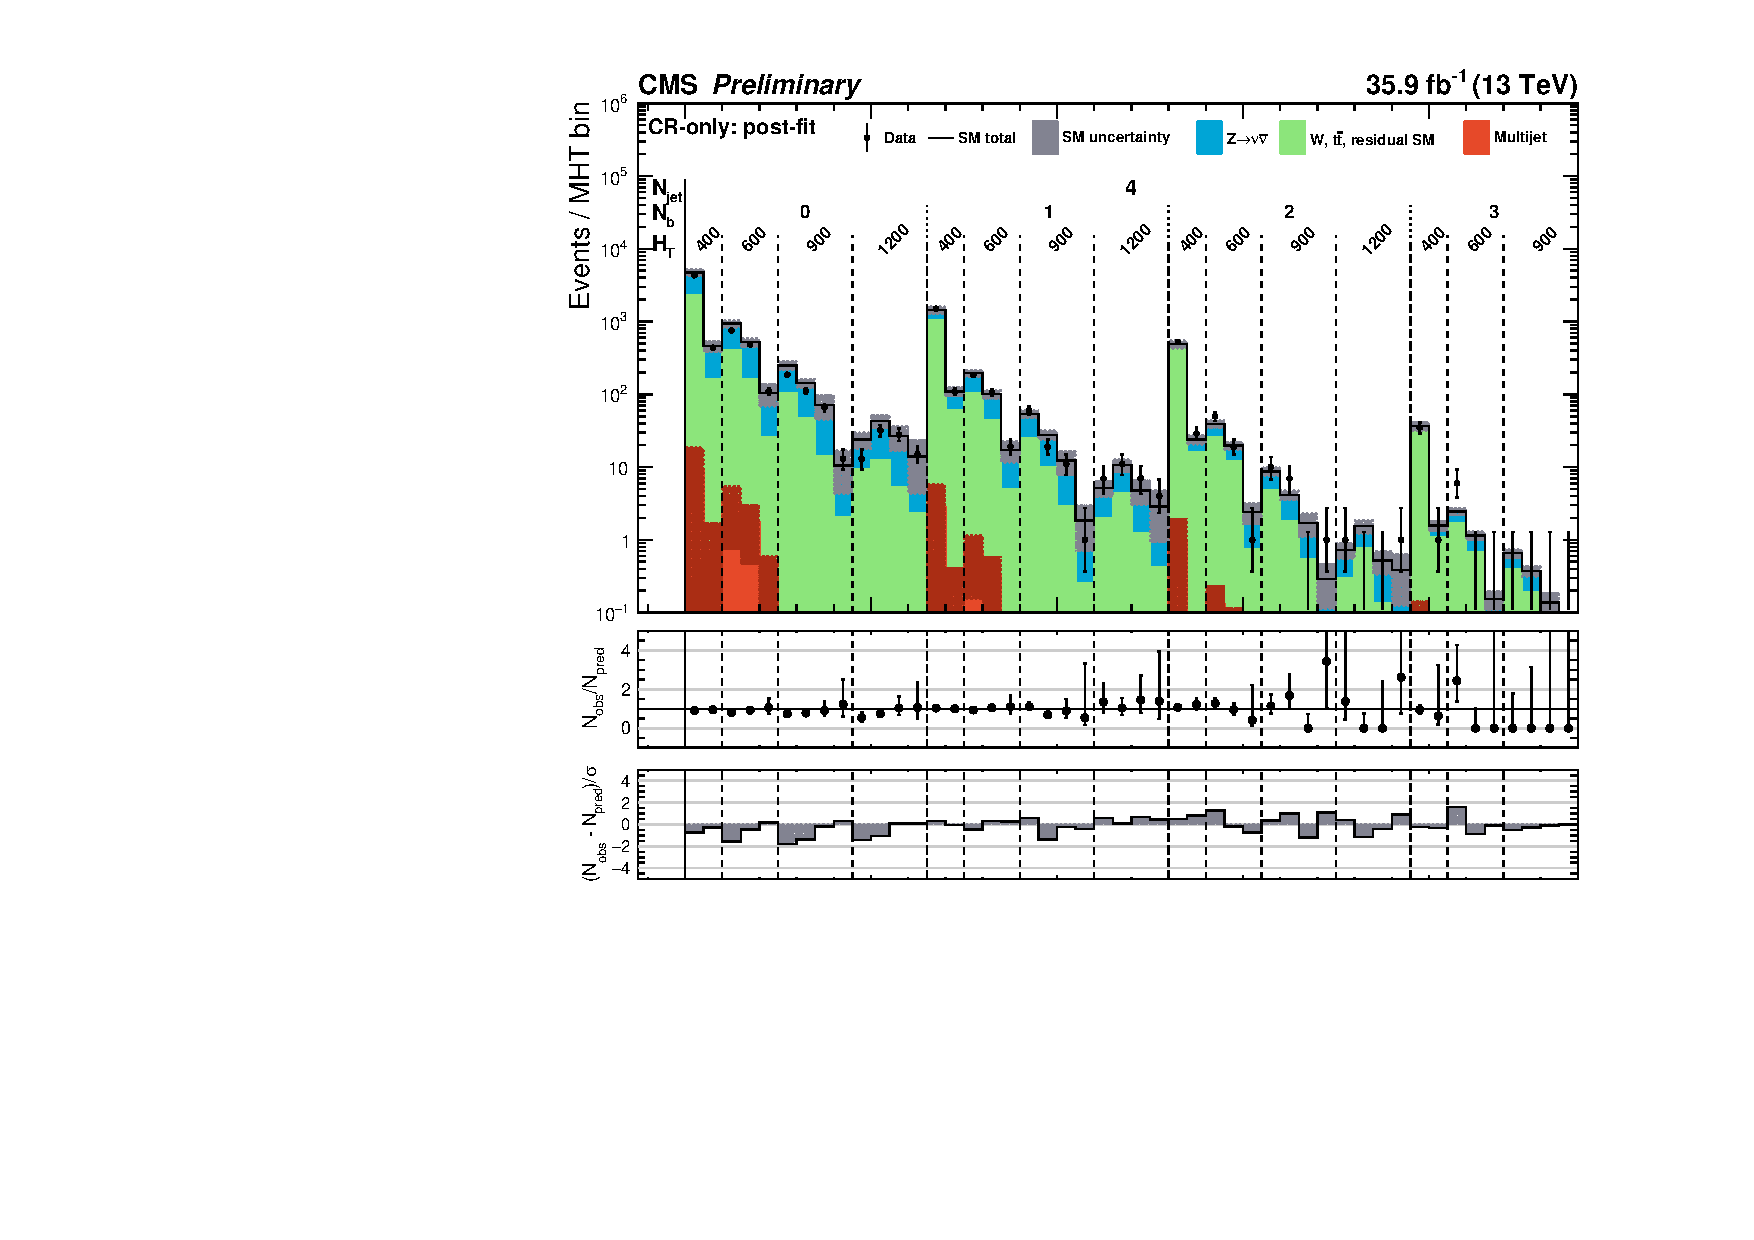
\includegraphics[width=0.48\textwidth]{figures/results/36invfb_preapproval/mht_binned/cr-only/4jet_cr-only.pdf}
  }\\
  \subfigure[\label{fig:cr-fit:five-jet}Topologies with 5 jets]{
    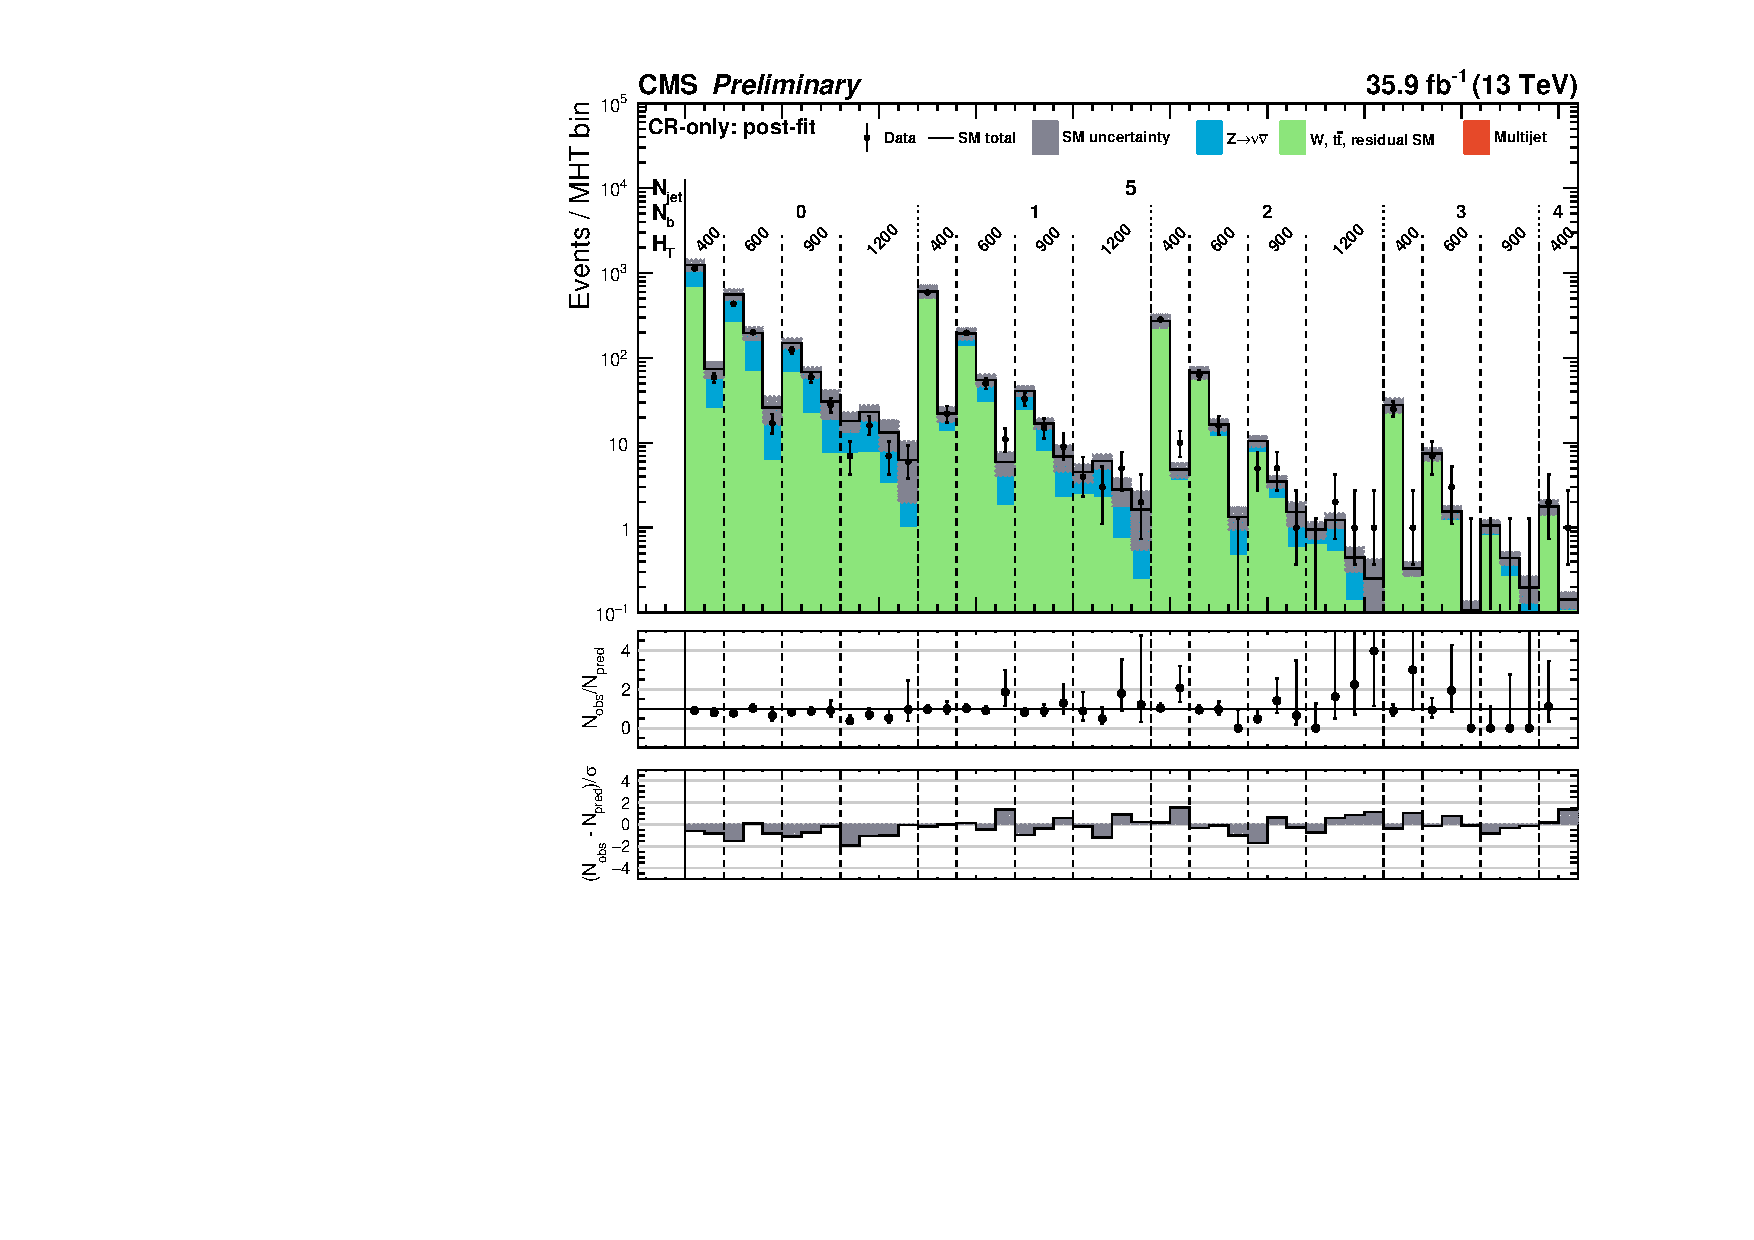
\includegraphics[width=0.48\textwidth]{figures/results/36invfb_preapproval/mht_binned/cr-only/5jet_cr-only.pdf}
  }~ 
  \subfigure[\label{fig:cr-fit:six-jet}Topologies with $\ge$6 jets]{
    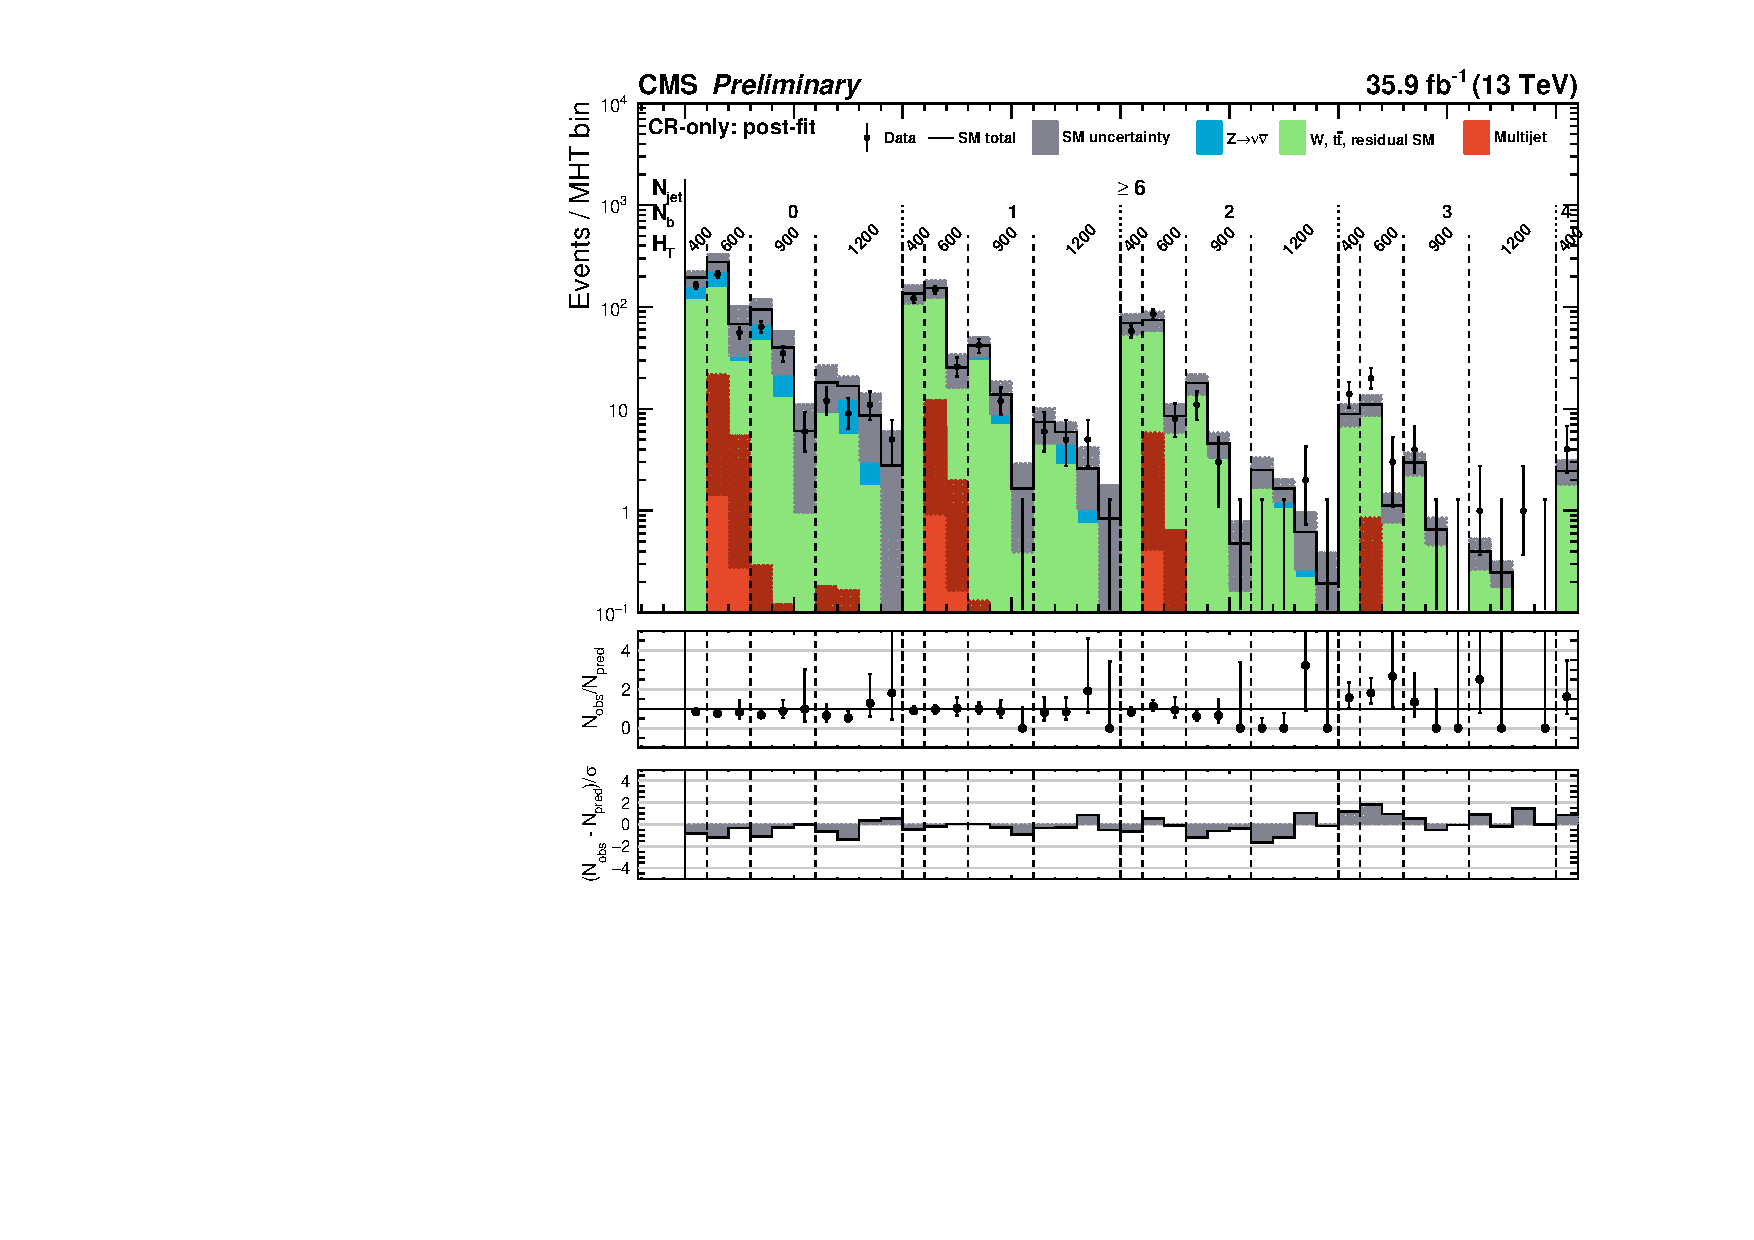
\includegraphics[width=0.48\textwidth]{figures/results/36invfb_preapproval/mht_binned/cr-only/6+_jets_cr-only.pdf}
  }\\
  \caption{\label{fig:cr-fit} Results of the control region-only fit in the 7 different event topologies.
  Top panels:  Event yields in data and SM expectations.
  Centre panels:  Ratio of the observed and expected counts.
  Bottom panels:  Observed pulls of the data from expectation.
  Detailed descriptions are given in the text.
	}
\end{figure}

\clearpage
\begin{figure}[!h]
  \centering
  \subfigure[\label{fig:full-fit:mono-asymm}Monojet and asymmetric topologies]{
    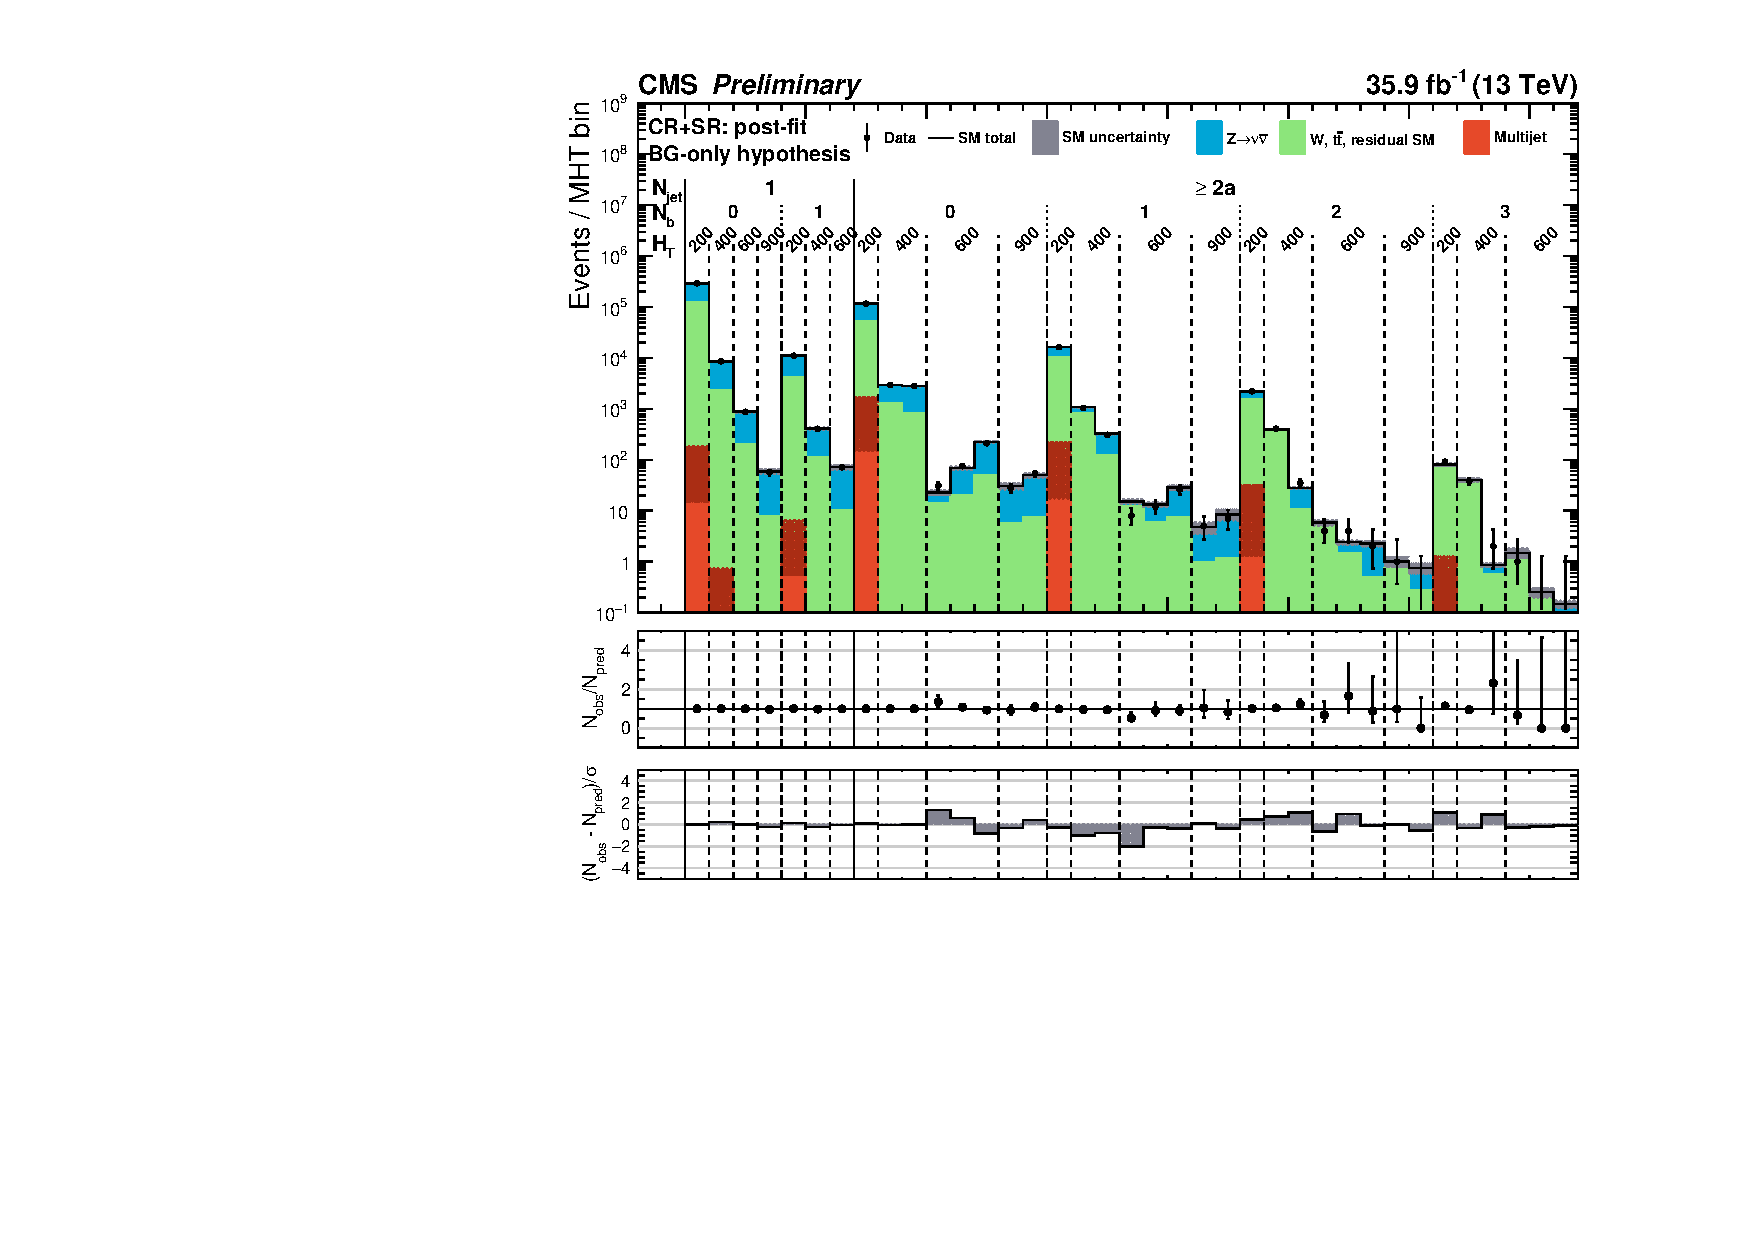
\includegraphics[width=0.48\textwidth]{figures/results/36invfb_preapproval/mht_binned/full-fit_bg/monojet_full-fit_bg.pdf}
  }~ 
  \subfigure[\label{fig:full-fit:dijet}Dijet topologies]{
    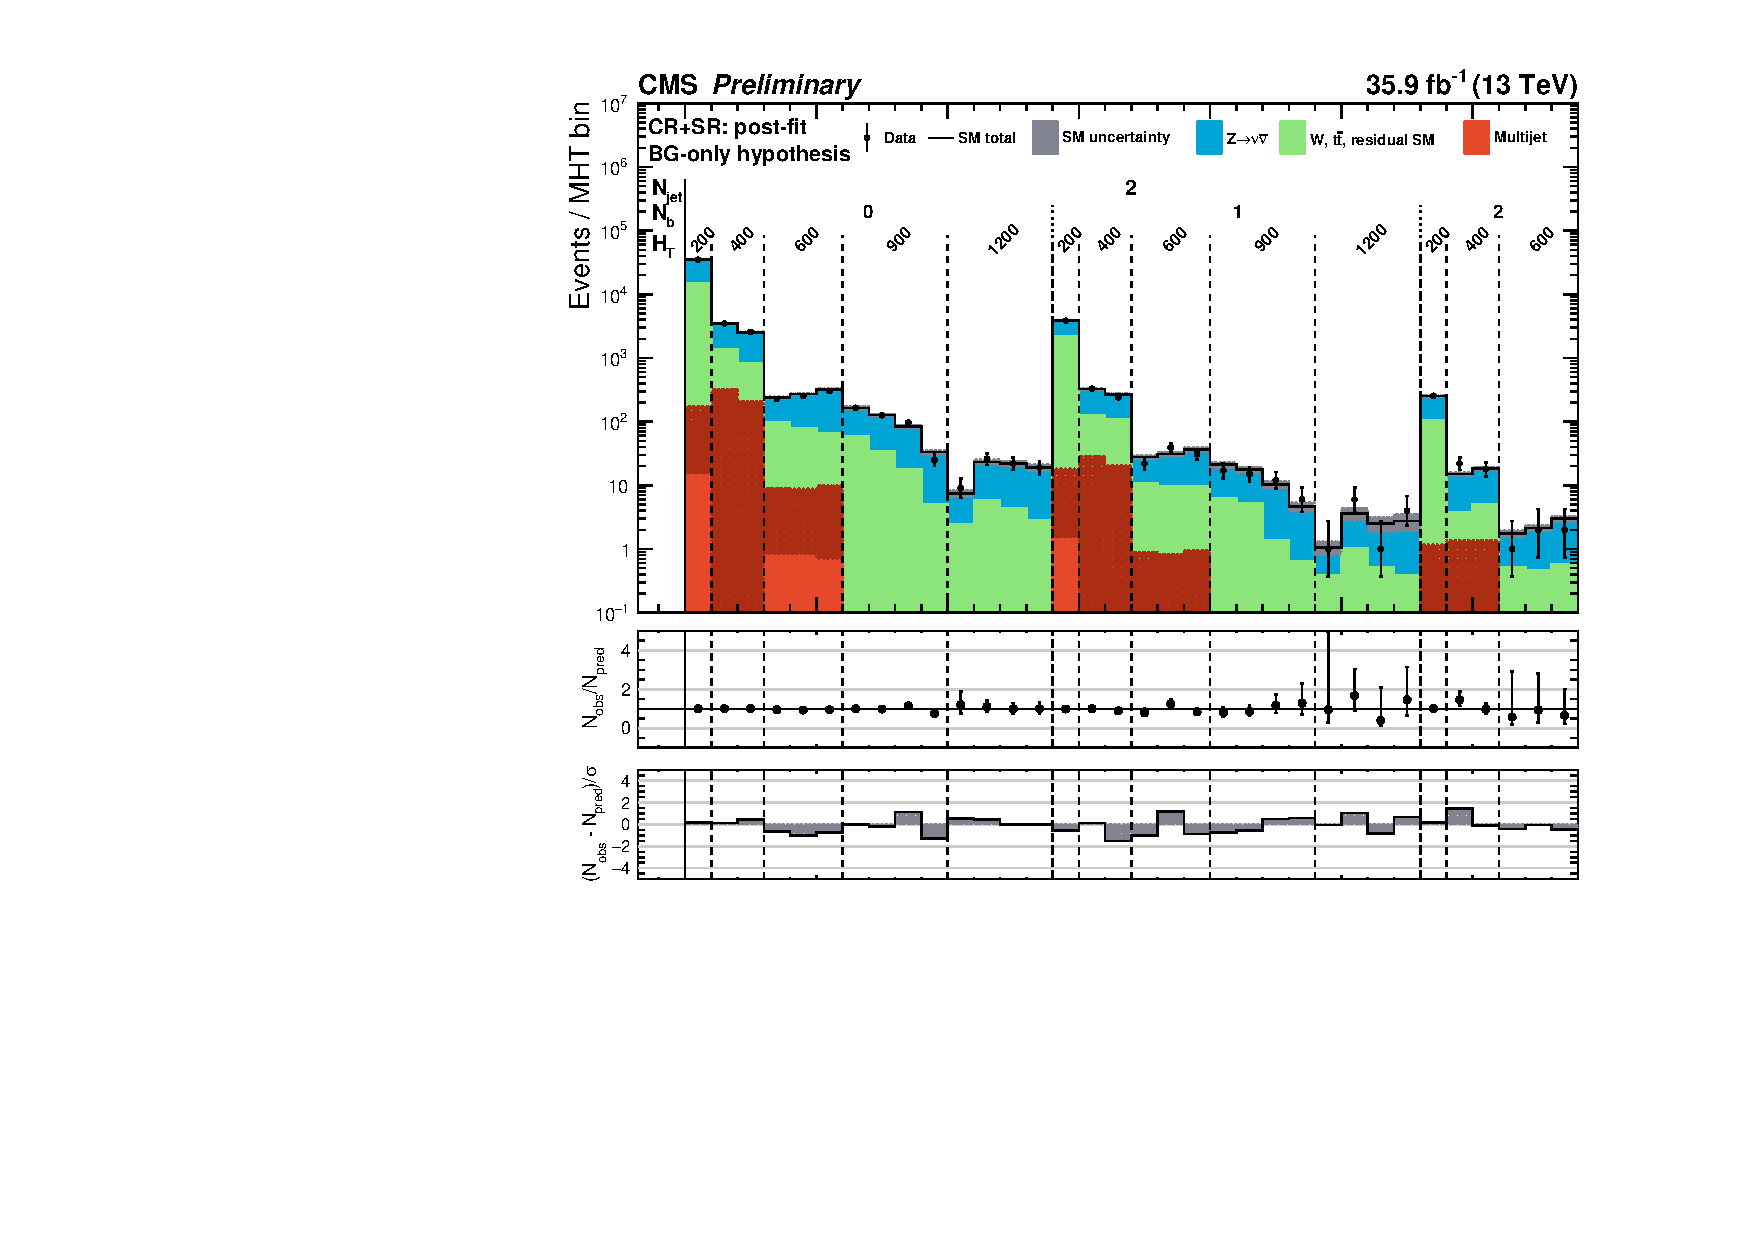
\includegraphics[width=0.48\textwidth]{figures/results/36invfb_preapproval/mht_binned/full-fit_bg/di-jet_full-fit_bg.pdf}
  }\\
  \subfigure[\label{fig:full-fit:three-jet}Topologies with 3 jets]{
    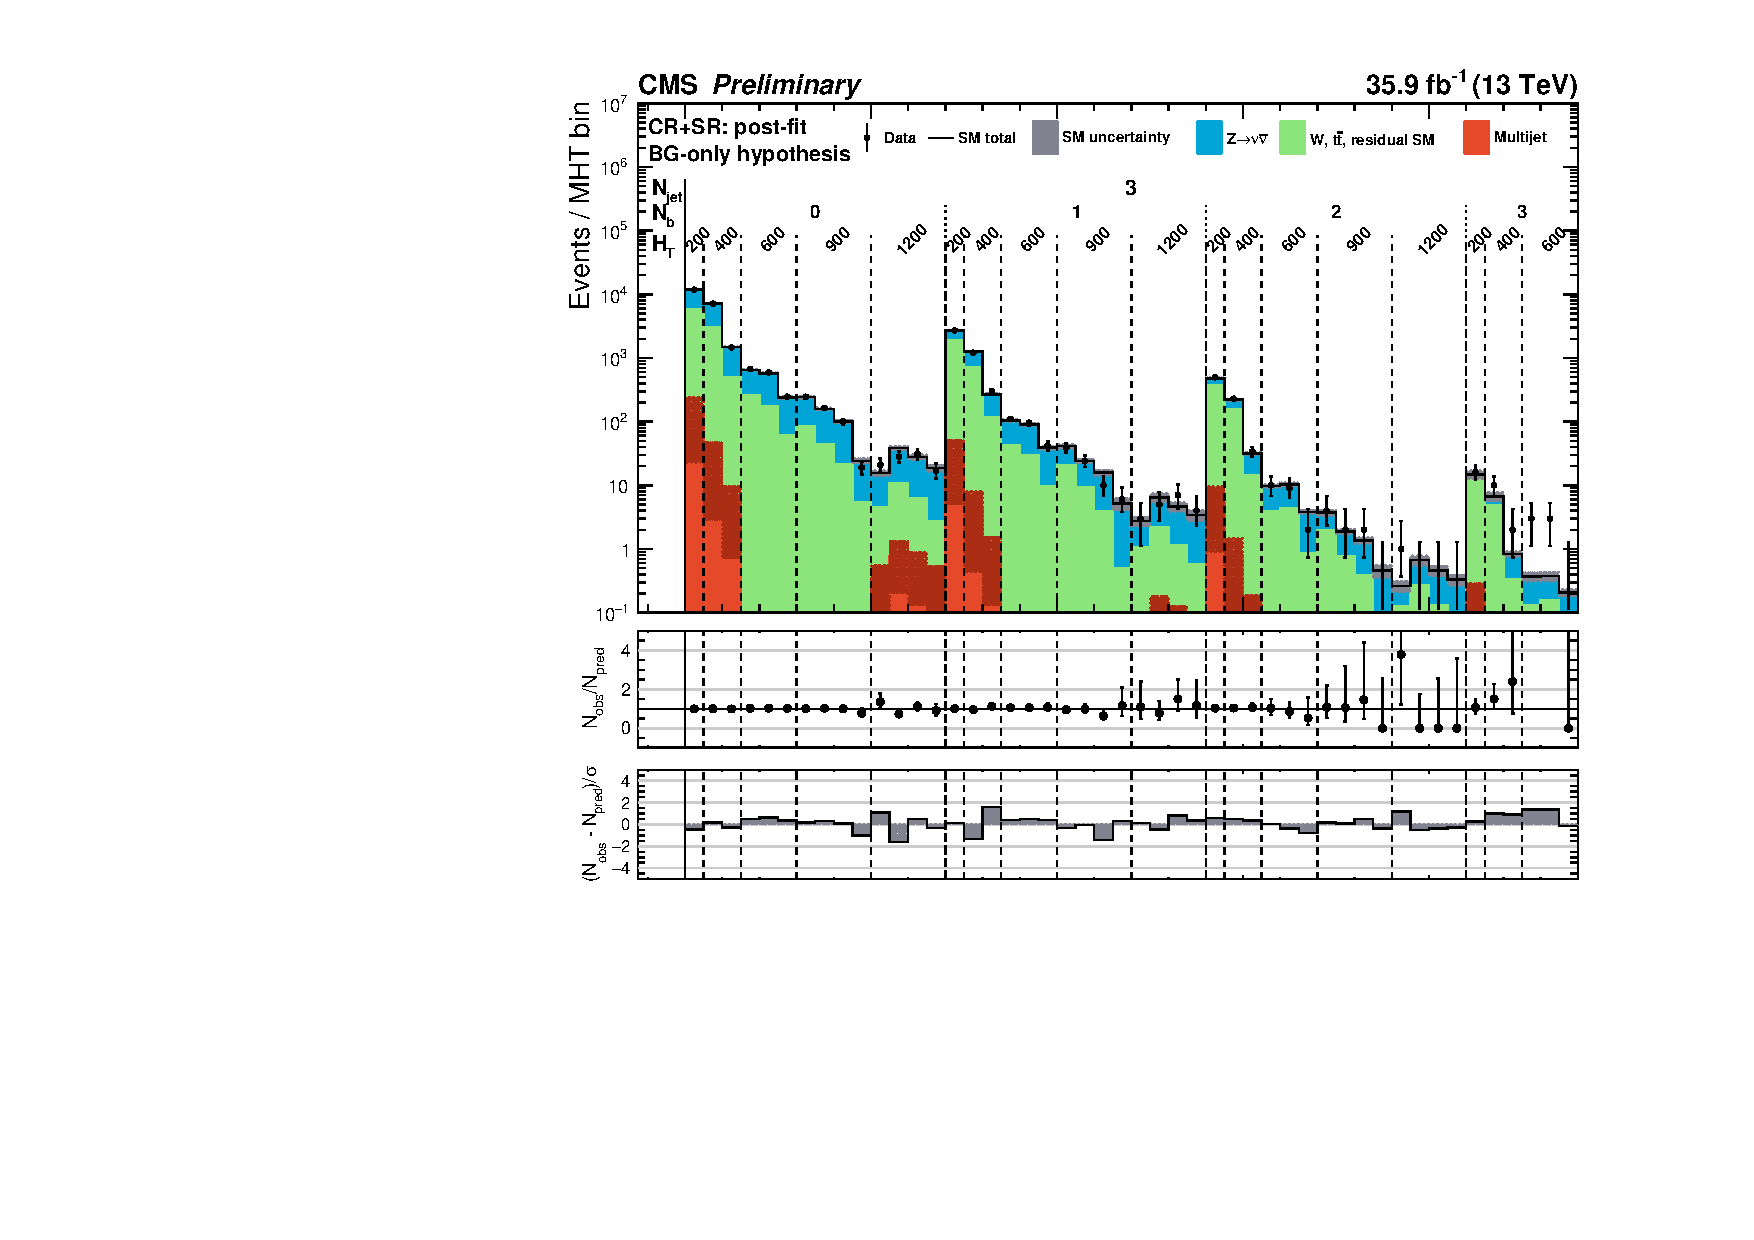
\includegraphics[width=0.48\textwidth]{figures/results/36invfb_preapproval/mht_binned/full-fit_bg/3jet_full-fit_bg.pdf}
  }~ 
  \subfigure[\label{fig:full-fit:four-jet}Topologies with 4 jets]{
    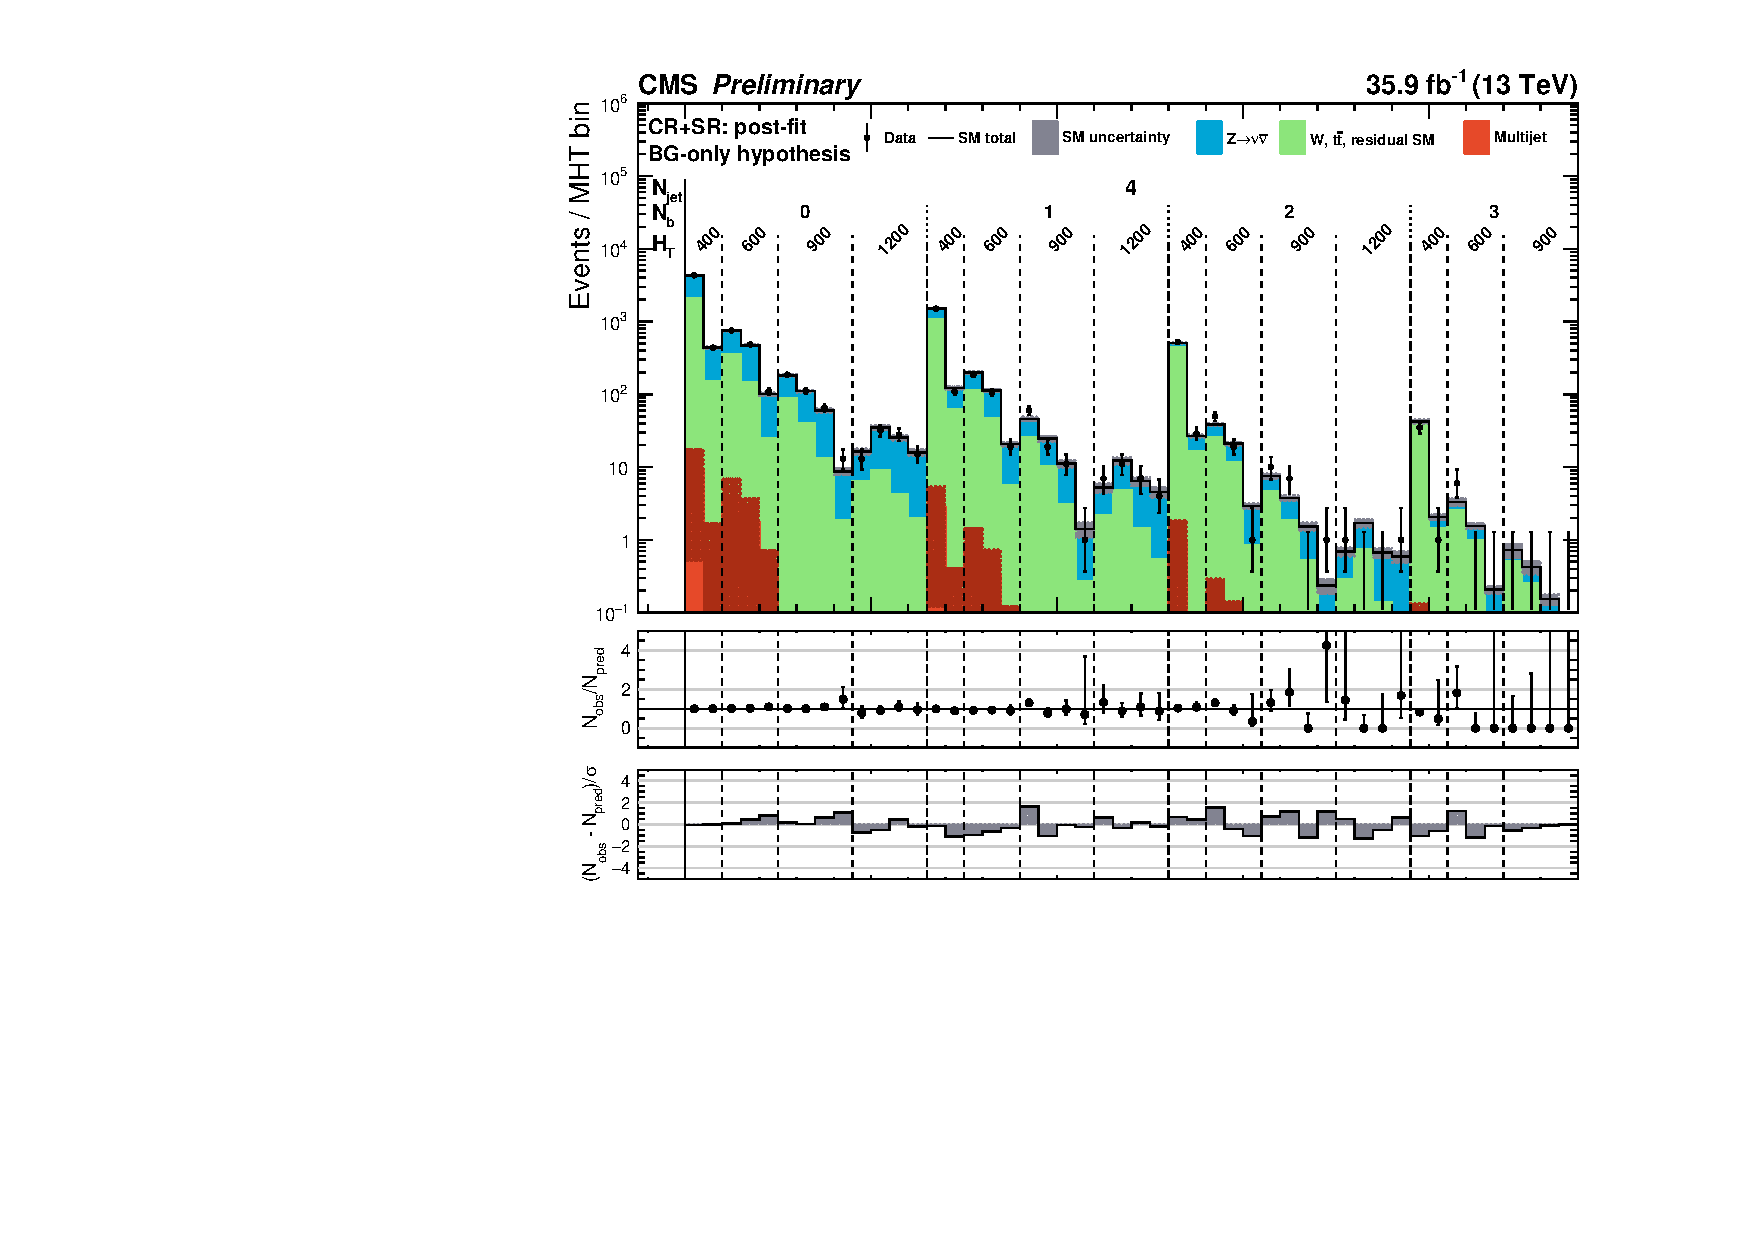
\includegraphics[width=0.48\textwidth]{figures/results/36invfb_preapproval/mht_binned/full-fit_bg/4jet_full-fit_bg.pdf}
  }\\
  \subfigure[\label{fig:full-fit:five-jet}Topologies with 5 jets]{
    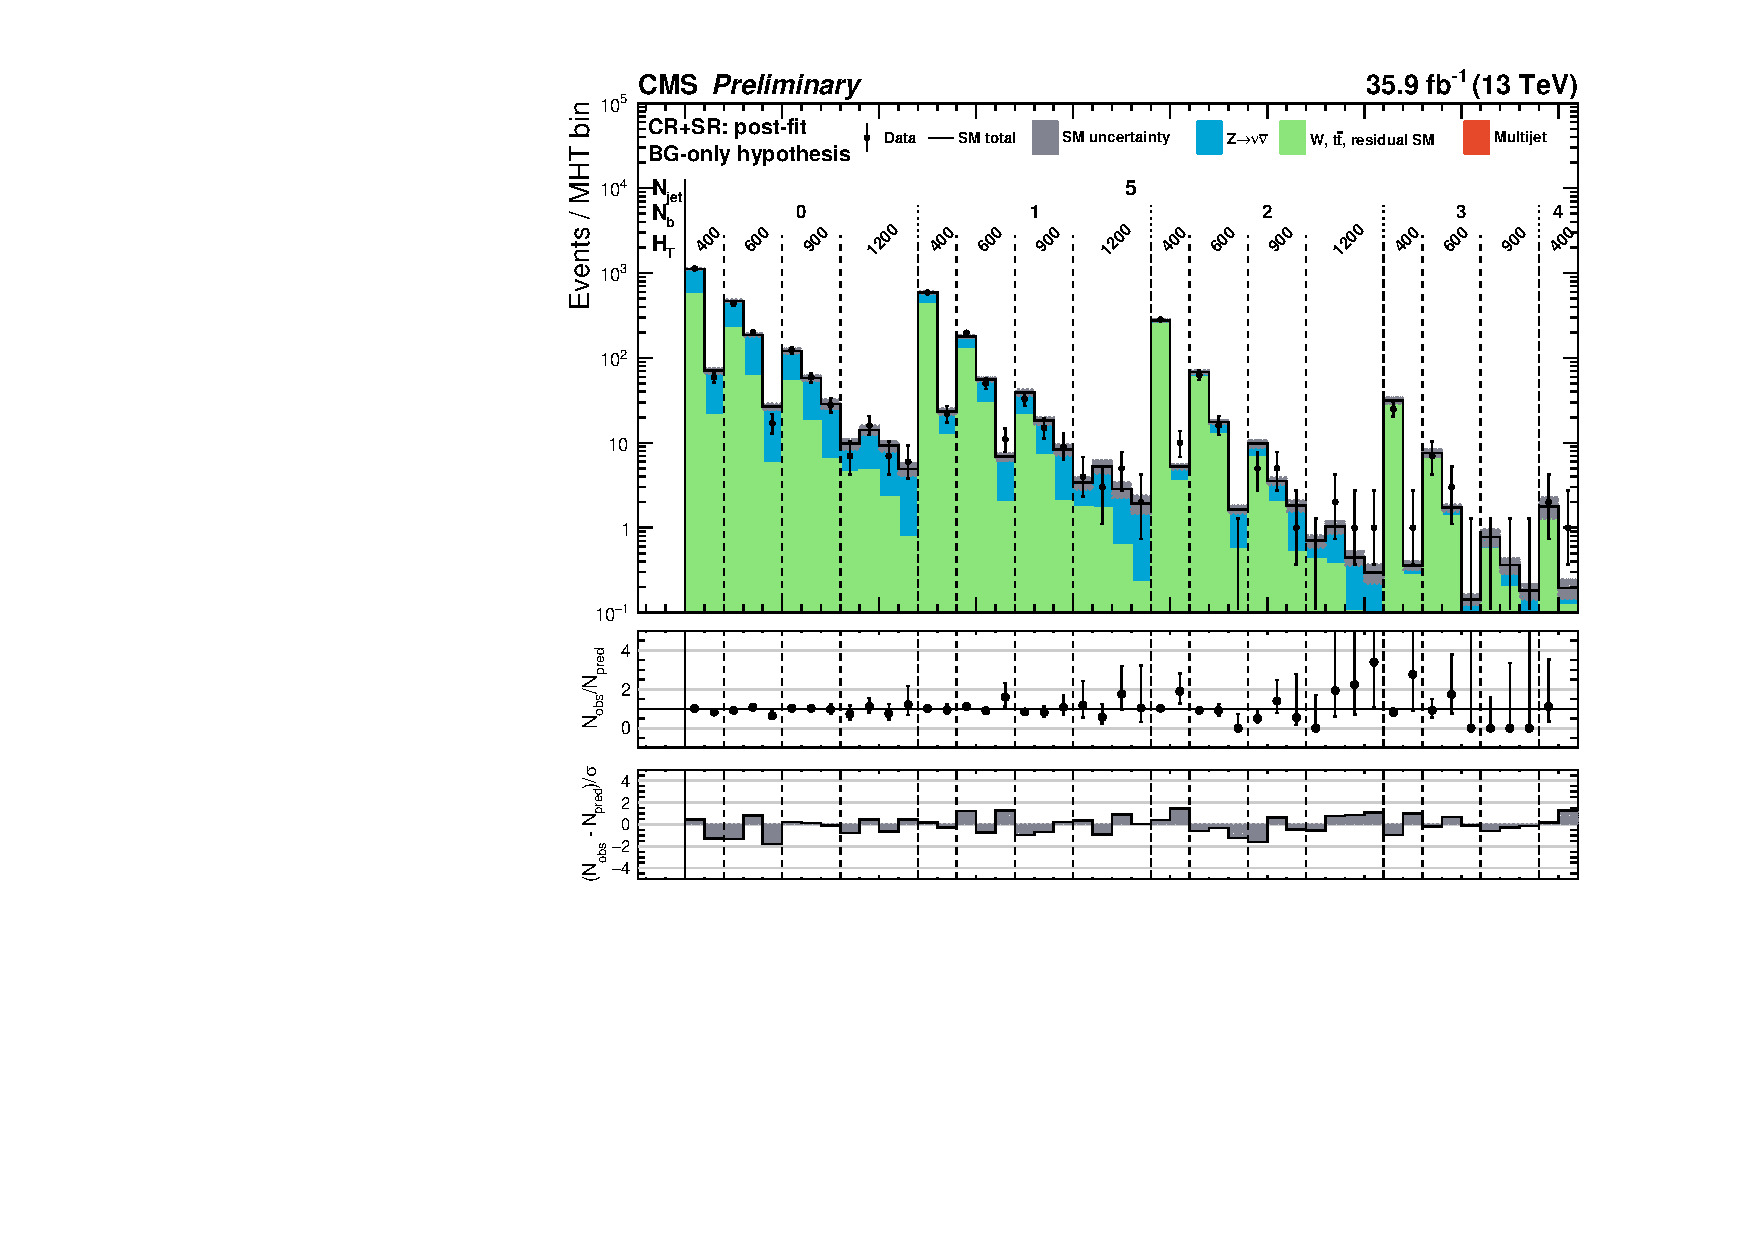
\includegraphics[width=0.48\textwidth]{figures/results/36invfb_preapproval/mht_binned/full-fit_bg/5jet_full-fit_bg.pdf}
  }~ 
  \subfigure[\label{fig:full-fit:six-jet}Topologies with $\ge$6 jets]{
    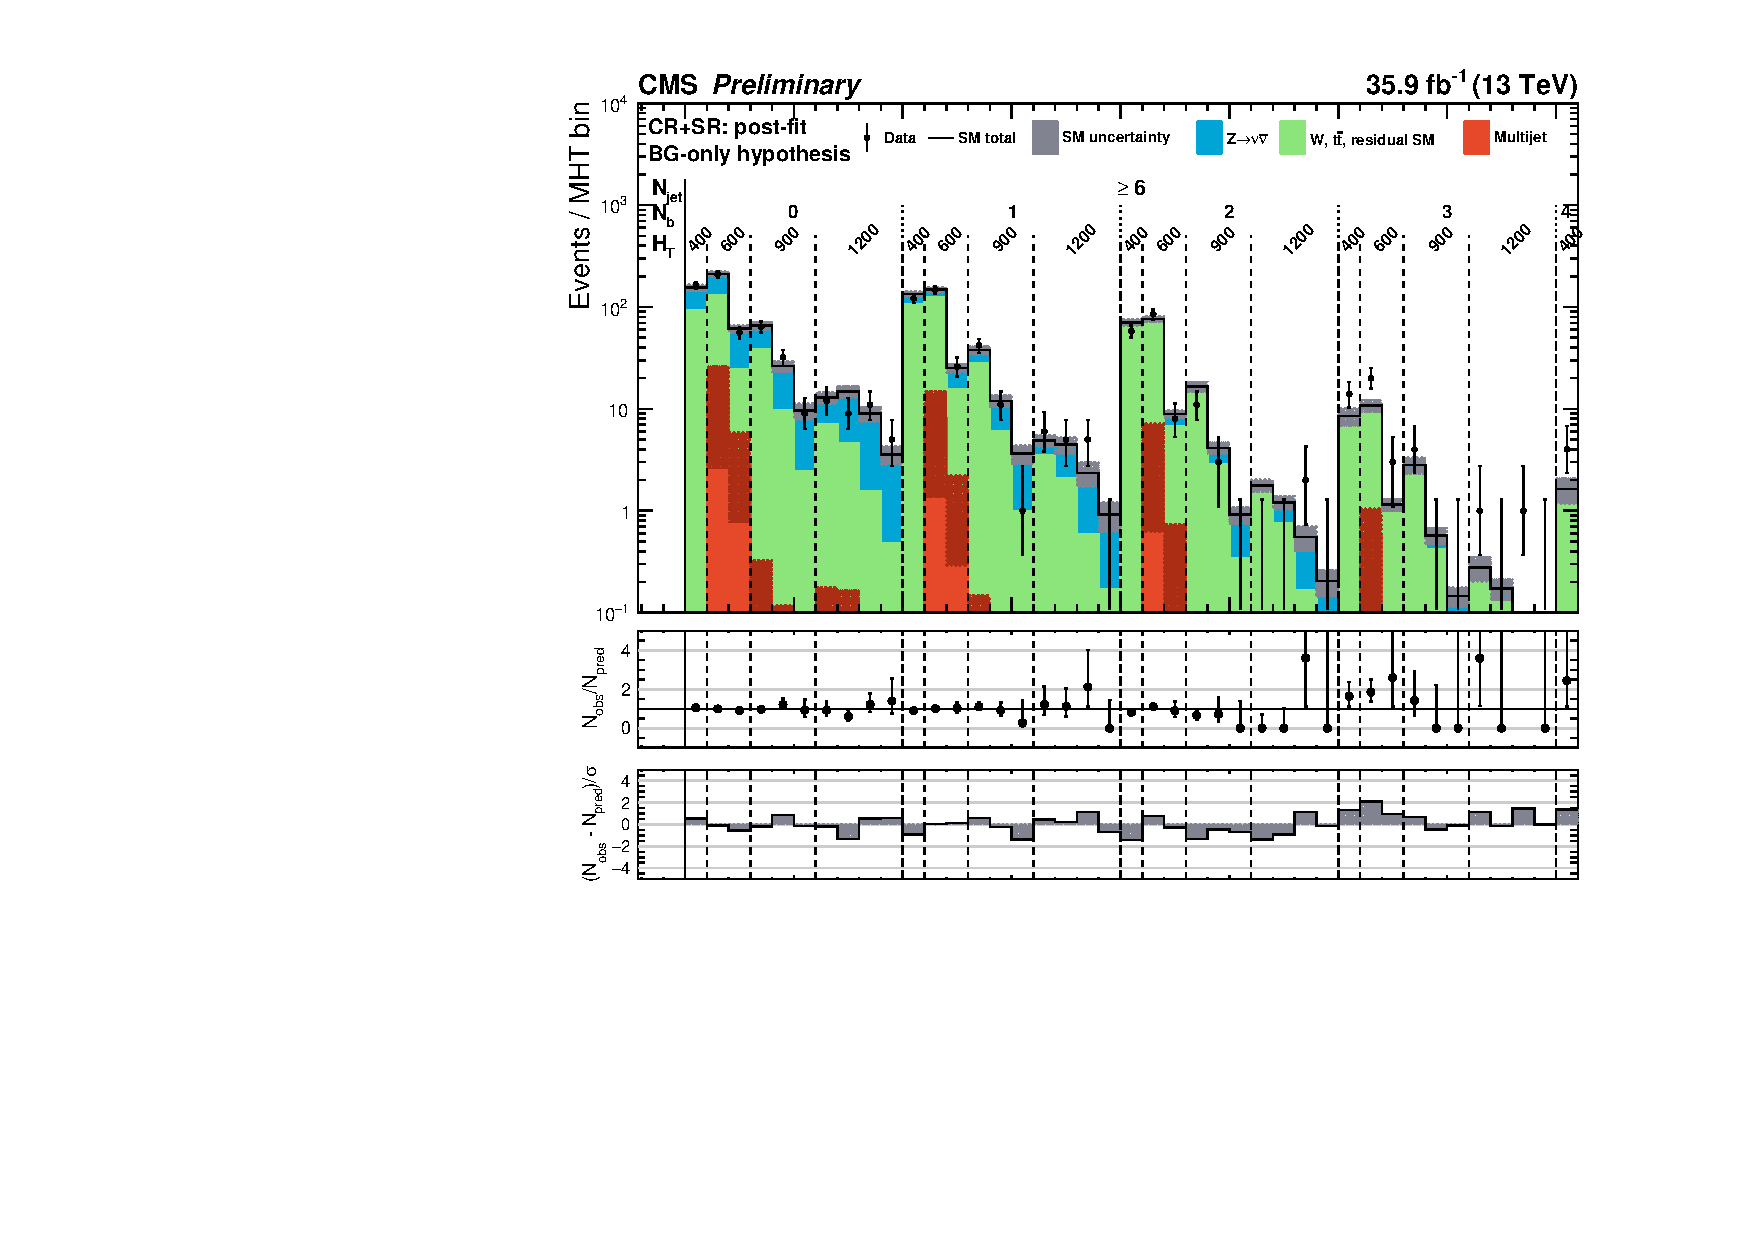
\includegraphics[width=0.48\textwidth]{figures/results/36invfb_preapproval/mht_binned/full-fit_bg/6+_jets_full-fit_bg.pdf}
  }\\
  \caption{\label{fig:full-fit} Results of the full fit in the 7 different event topologies.
  Top panels:  Event yields in data and SM expectations.
  Centre panels:  Ratio of the observed and expected counts.
  Bottom panels:  Observed pulls of the data from expectation.
  Detailed descriptions are given in the text.
	}
\end{figure}

% 1d histograms 
\clearpage
\subsubsection{Ratios and pulls}

\begin{figure}[h!]
  \centering
  \caption{(Left) Data-to-background ratios for all event categories,
    with counts integrated over \mht, obtained from the masked
    fit. (Right) Pulls for all event categories, with counts
    integrated over \mht, obtained from the masked fit.}
  \label{fig:ratios_and_pulls}
  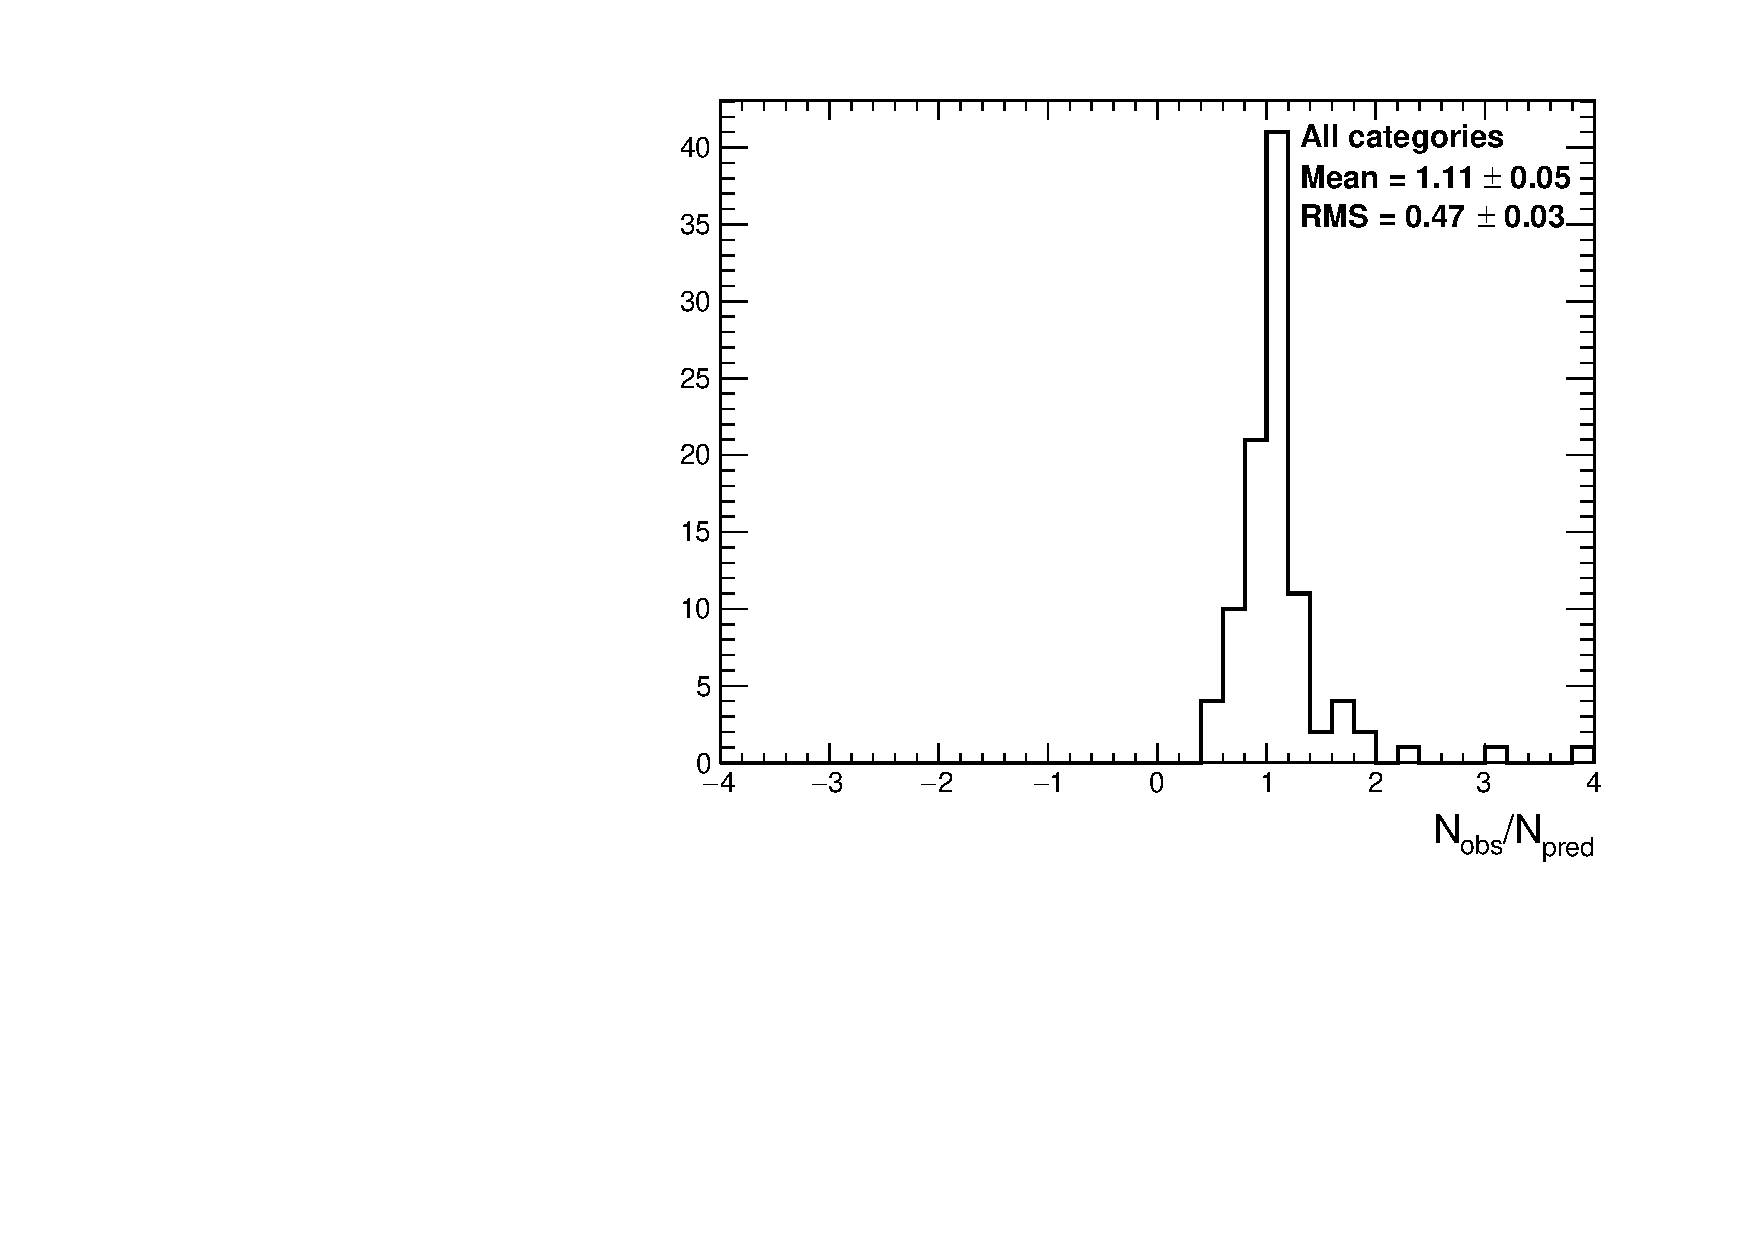
\includegraphics[width=0.49\linewidth]{figures/results/36invfb_preapproval/all/ratios_all_prefit.pdf}
  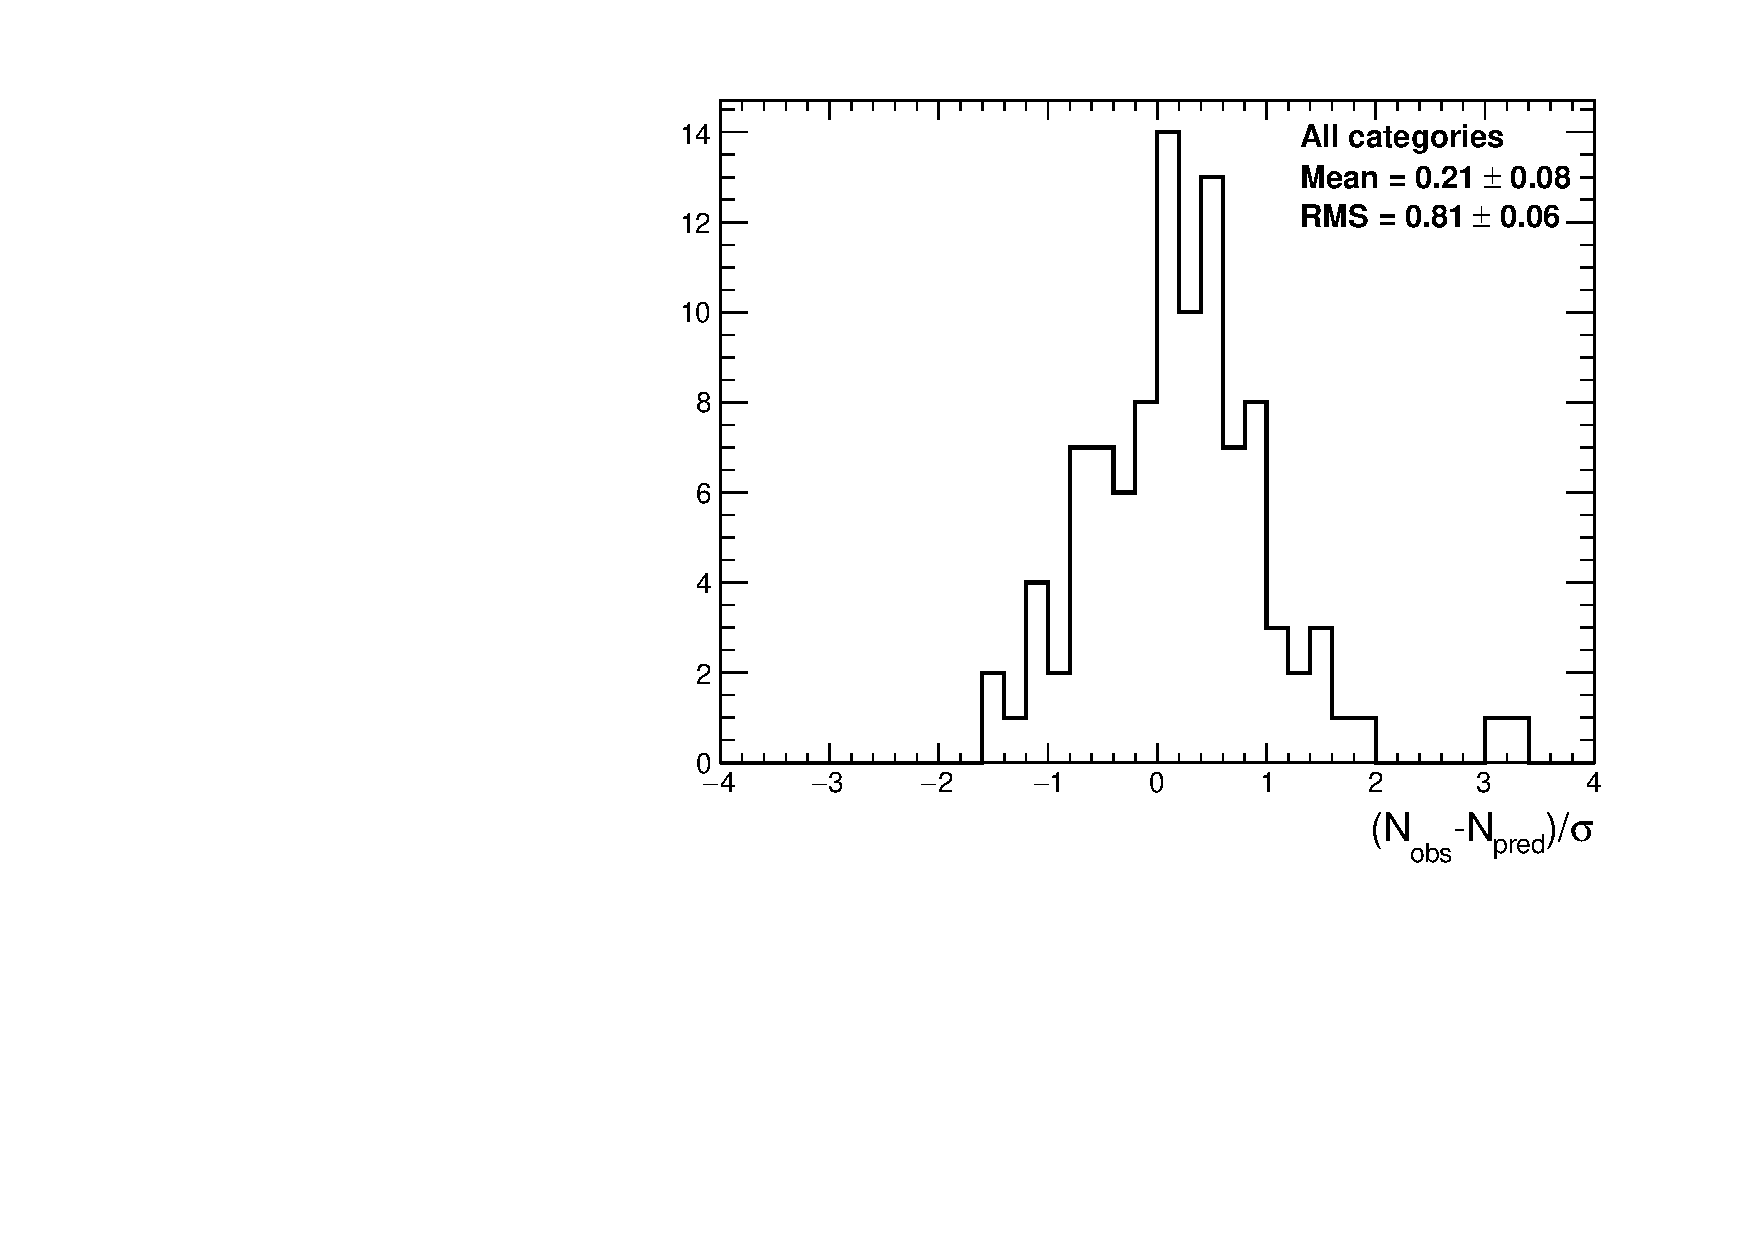
\includegraphics[width=0.49\linewidth]{figures/results/36invfb_preapproval/all/pulls_all_prefit.pdf}
\end{figure}

\begin{figure}[h!]
  \centering
  \caption{Pulls as a function of (\njet, \nb) event category and
    \scalht [GeV], with counts integrated over \mht, obtained from the
    masked fit.}
  \label{fig:pulls}
  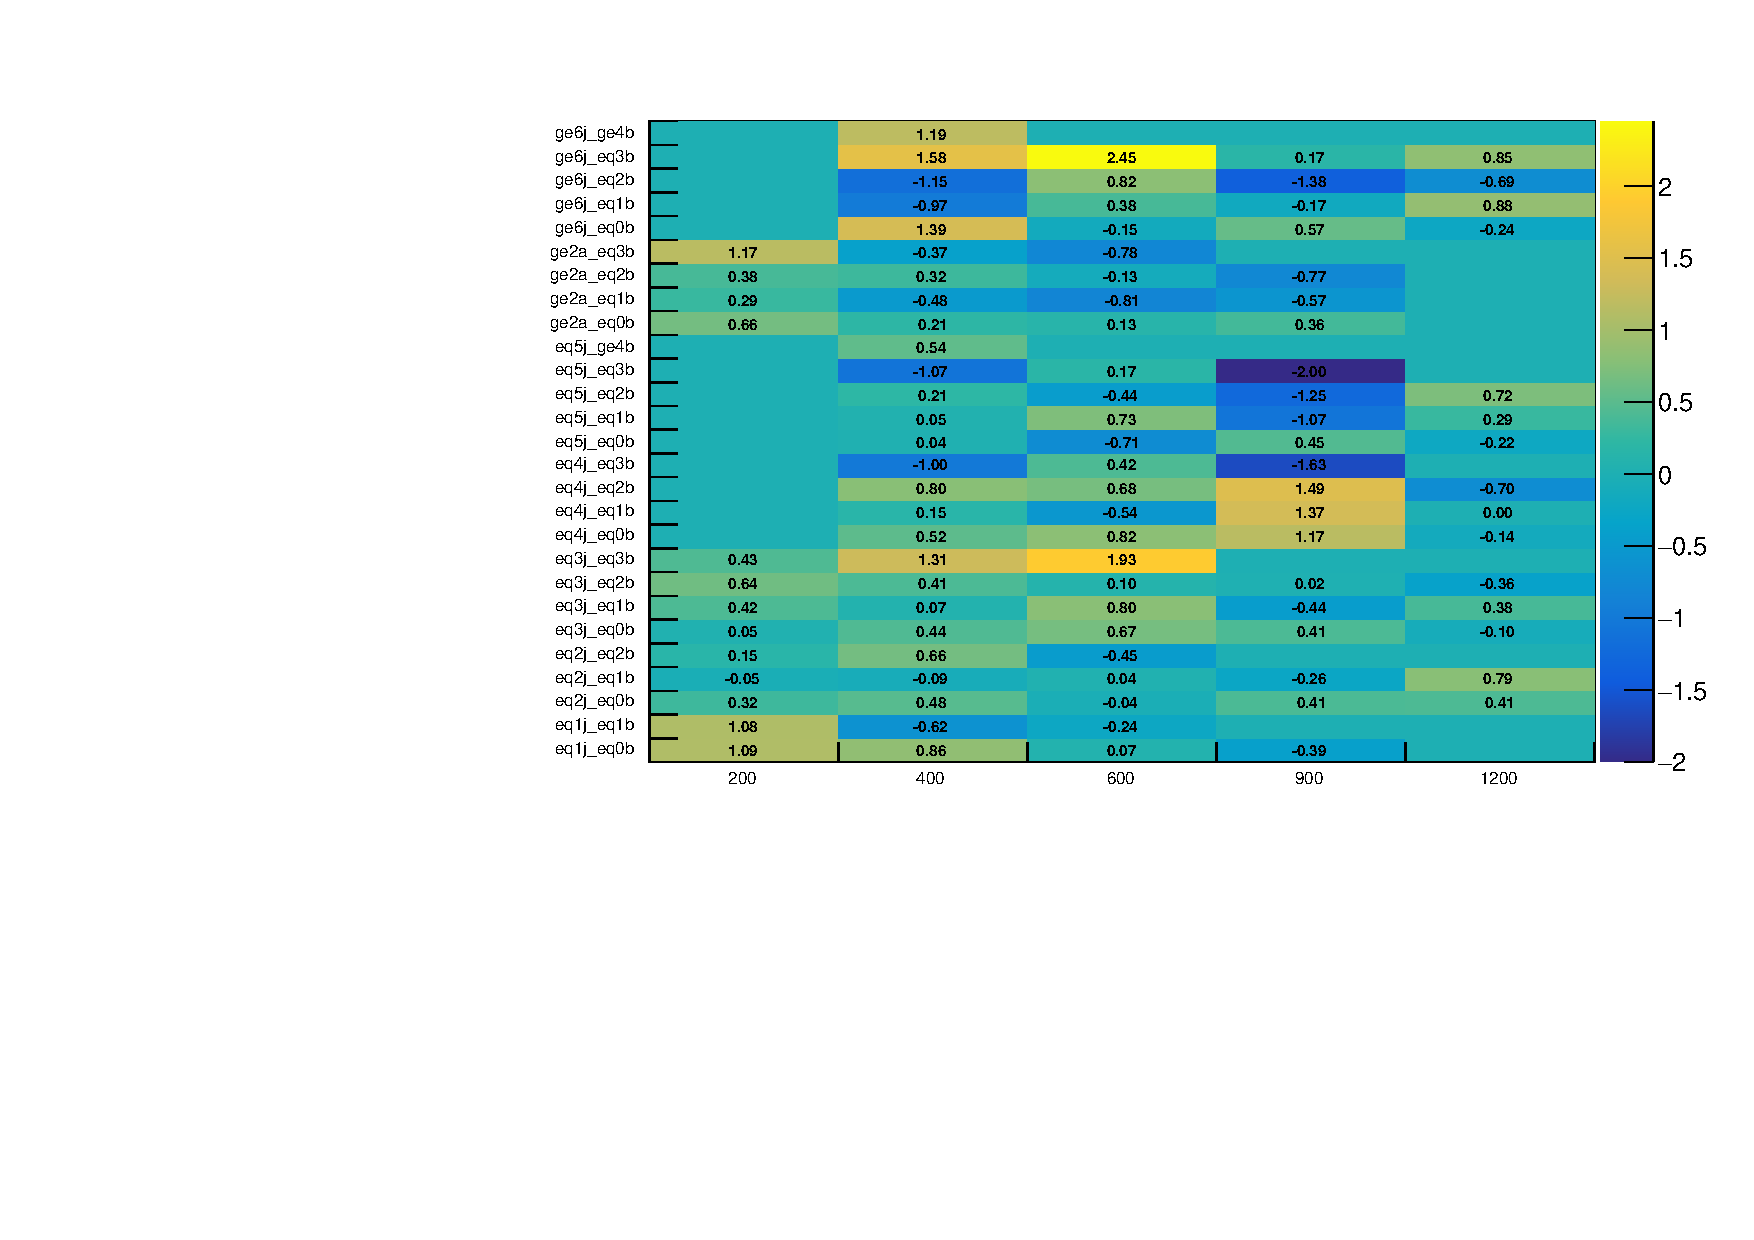
\includegraphics[width=0.8\linewidth]{figures/results/36invfb_preapproval/all/pull2D_CROnlyFit.pdf}
\end{figure}

\clearpage
\subsubsection{SM breakdown}

\begin{figure}[h!]
  \centering
  \caption{Breakdown of SM backgrounds in the signal region as
    determined by the CR-only (top) and full (bottom) fits.}
  \label{fig:breakdown}
  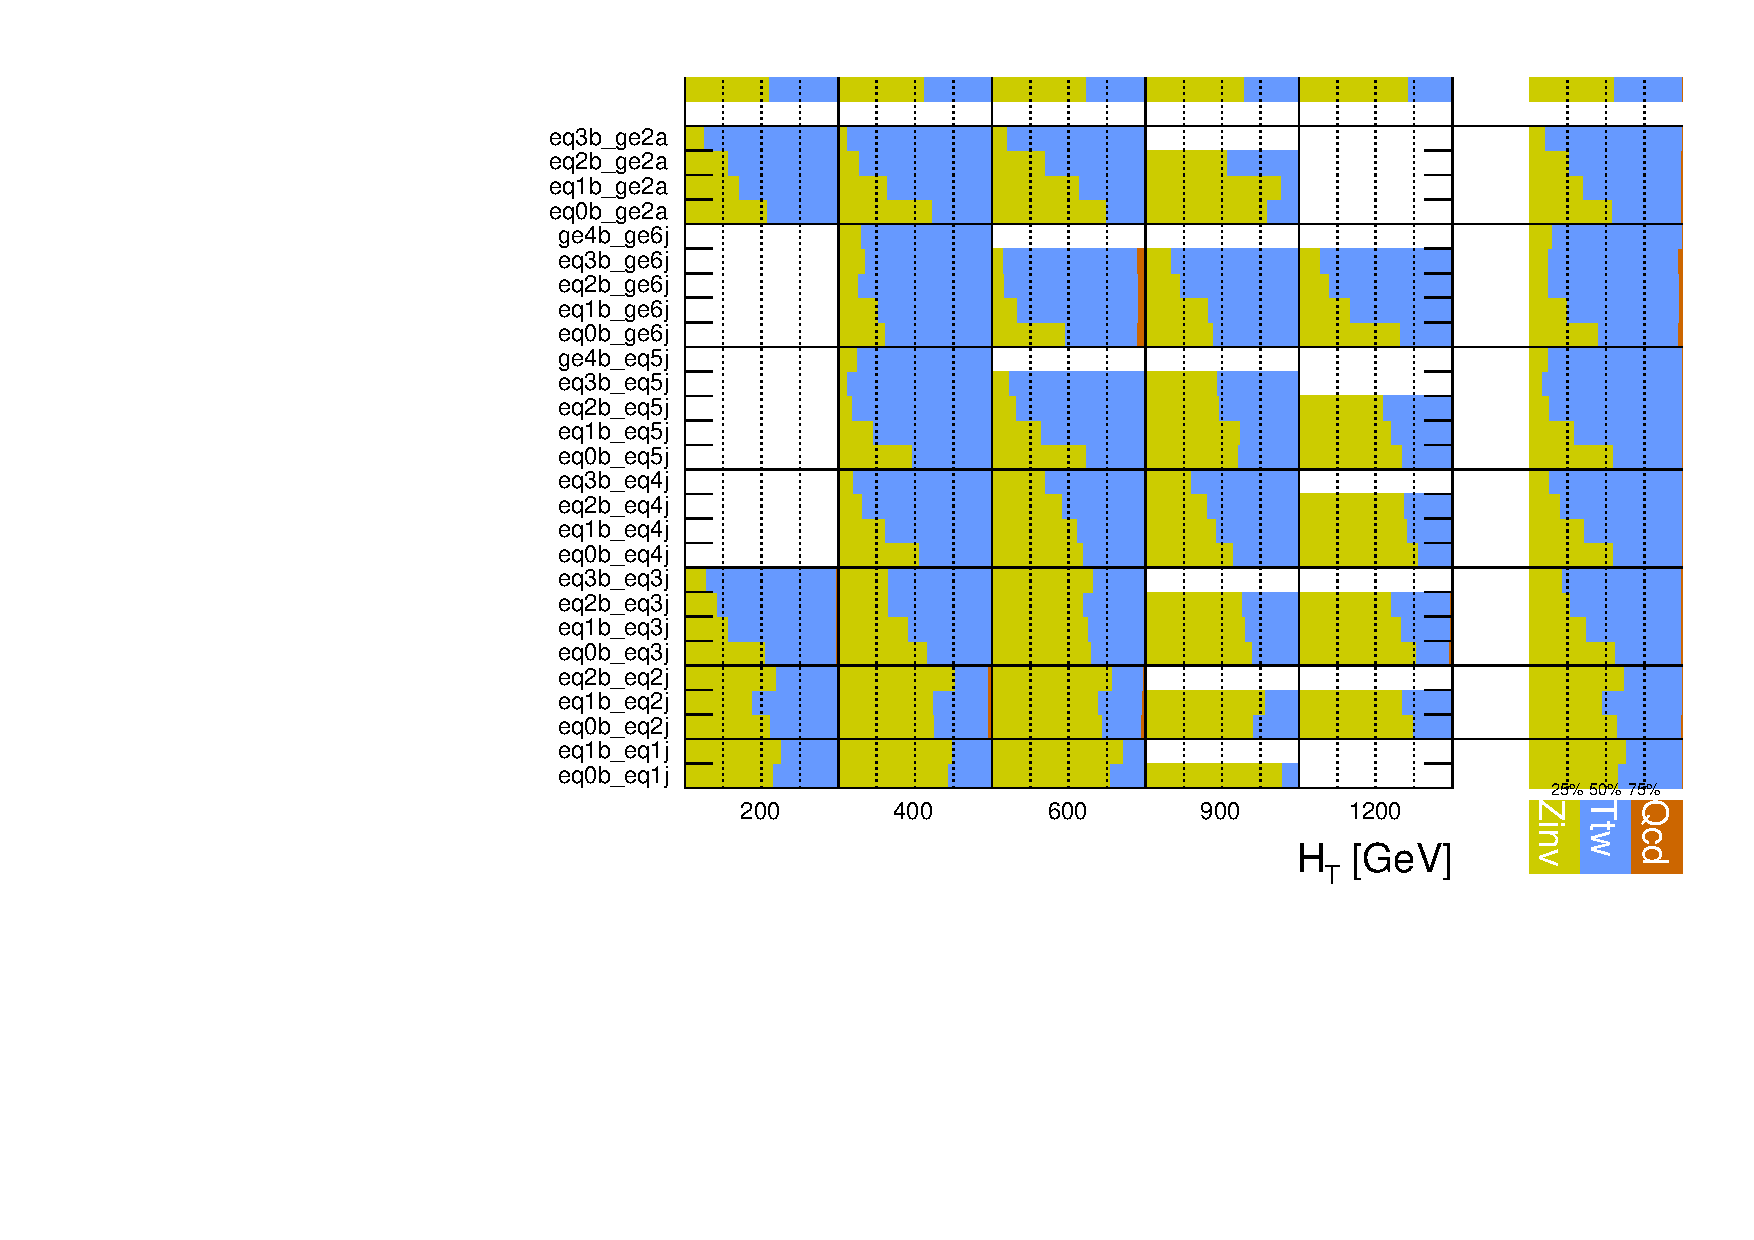
\includegraphics[width=0.8\linewidth]{figures/results/36invfb/breakdown/crfit/Signal_sample_composition.pdf}\\
  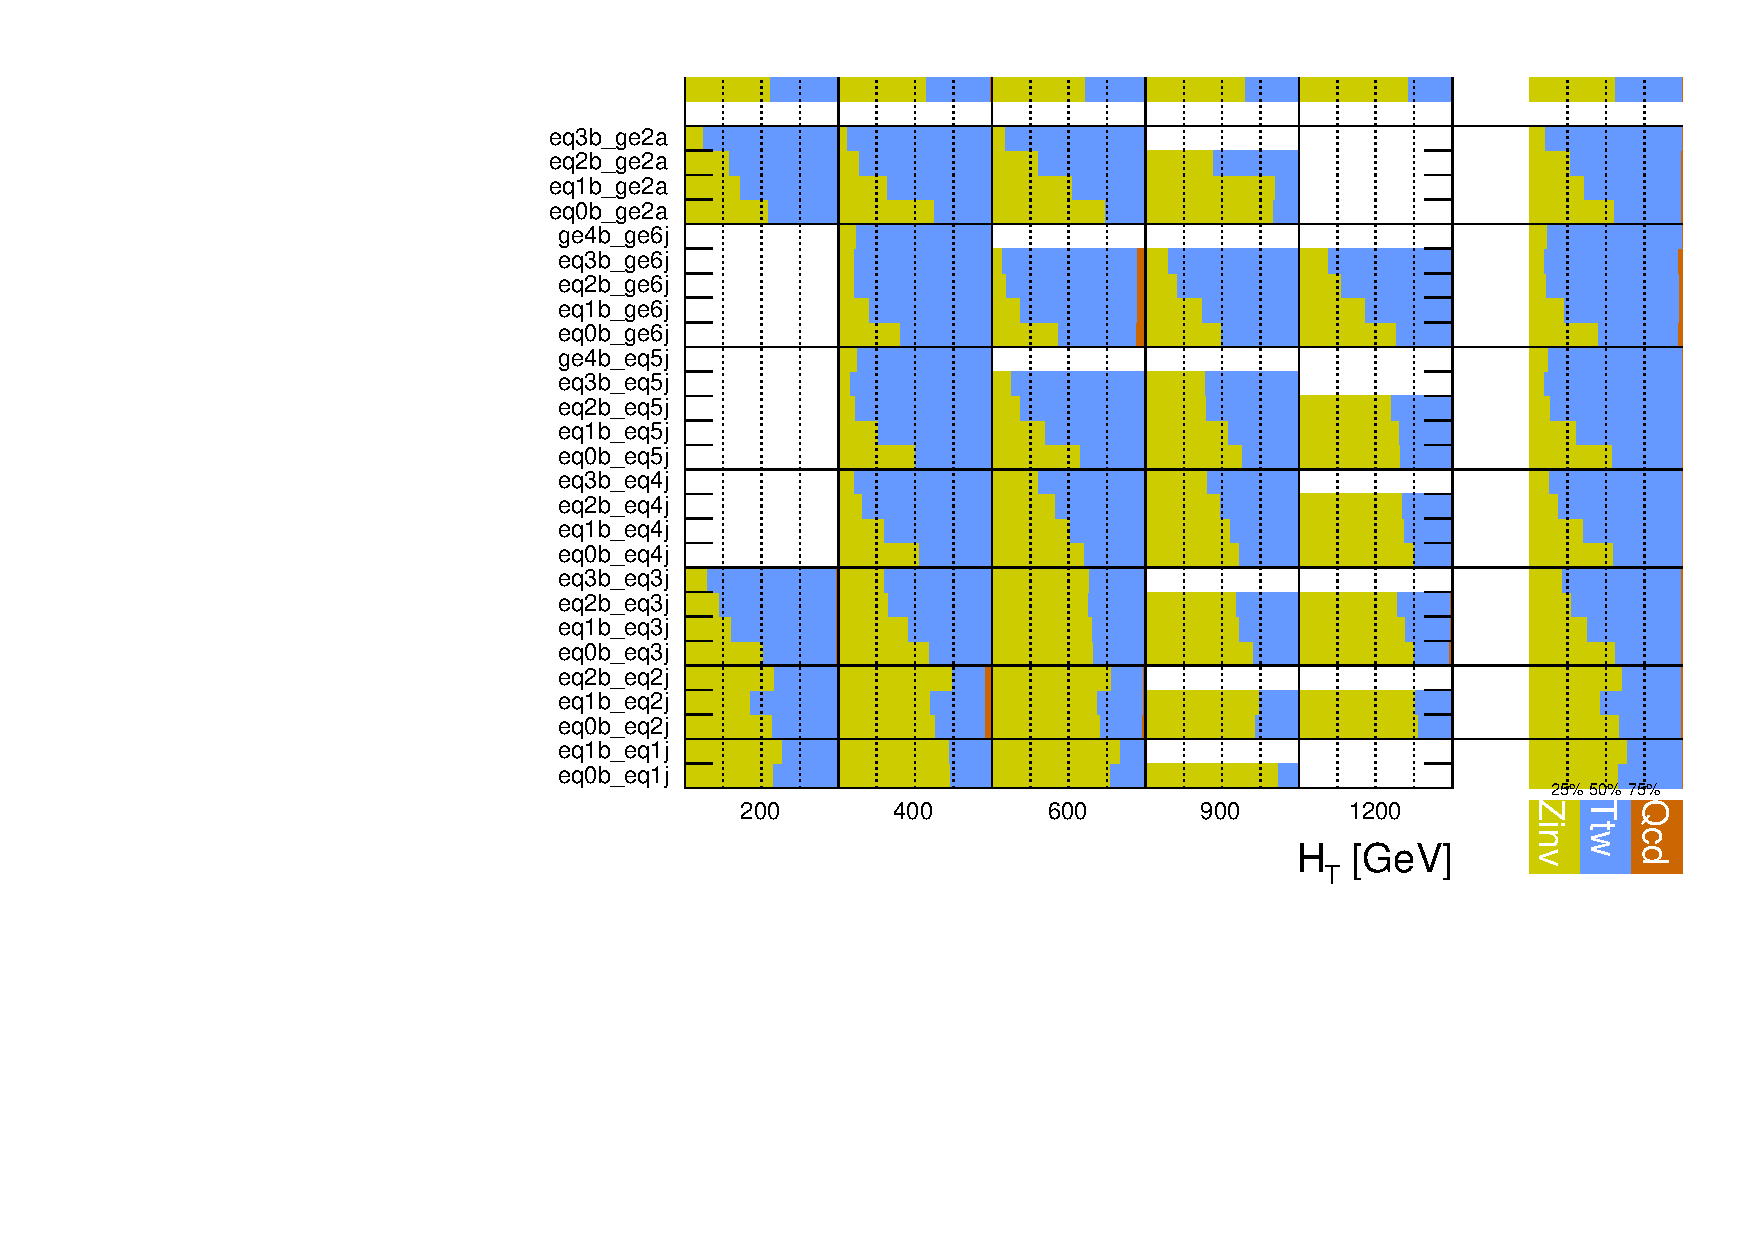
\includegraphics[width=0.8\linewidth]{figures/results/36invfb/breakdown/postfit/Signal_sample_composition.pdf}
\end{figure}

\clearpage
\subsection{Aggregated signal regions}
\label{sec:aggregated-results}

Observed data counts and SM background estimates are presented in
Figs.~\ref{fig:aggregated_results1}, \ref{fig:aggregated_results2},
\ref{fig:aggregated_results3}, and \ref{fig:aggregated_results4} for
the aggregated signal regions based on a simplified binning scheme, as
defined in Sec.~\ref{sec:aggregated}. The SM background estimates are
based on the same likelihood model used to determine the nominal
result.

\newcommand{\customcaption}[5]{(Upper panel) Event yields observed in
  data (solid circles) and SM expectations with their associated
  uncertainties (blue histogram with grey shaded band) determined from
  a simultaneous fit to data in the control regions only (CR-only
  fit). Event yields and expectations are shown as a function of
  \HTmiss for events in the #1 topology that are required to satisfy
  #2, #3, and (\cmsLeft) #4 or (\cmsRight) #5. 
  (Lower panel) The significance of deviations (pulls) observed in
  data with respect to both the SM expectations from the CR-only fit,
  expressed in terms of the total uncertainty in the SM
  expectations. The pulls cannot be considered independently due to
  inter-bin correlations.}

\clearpage
\begin{figure}[h!]
  \centering
  \caption{
    \customcaption{``monojet-like''}{$\njet = 1$ or $\njet = 2${\it a}}{$\scalht > 200\GeV$}{$\nb = 0$}{$\nb \geq 1$}
  }
  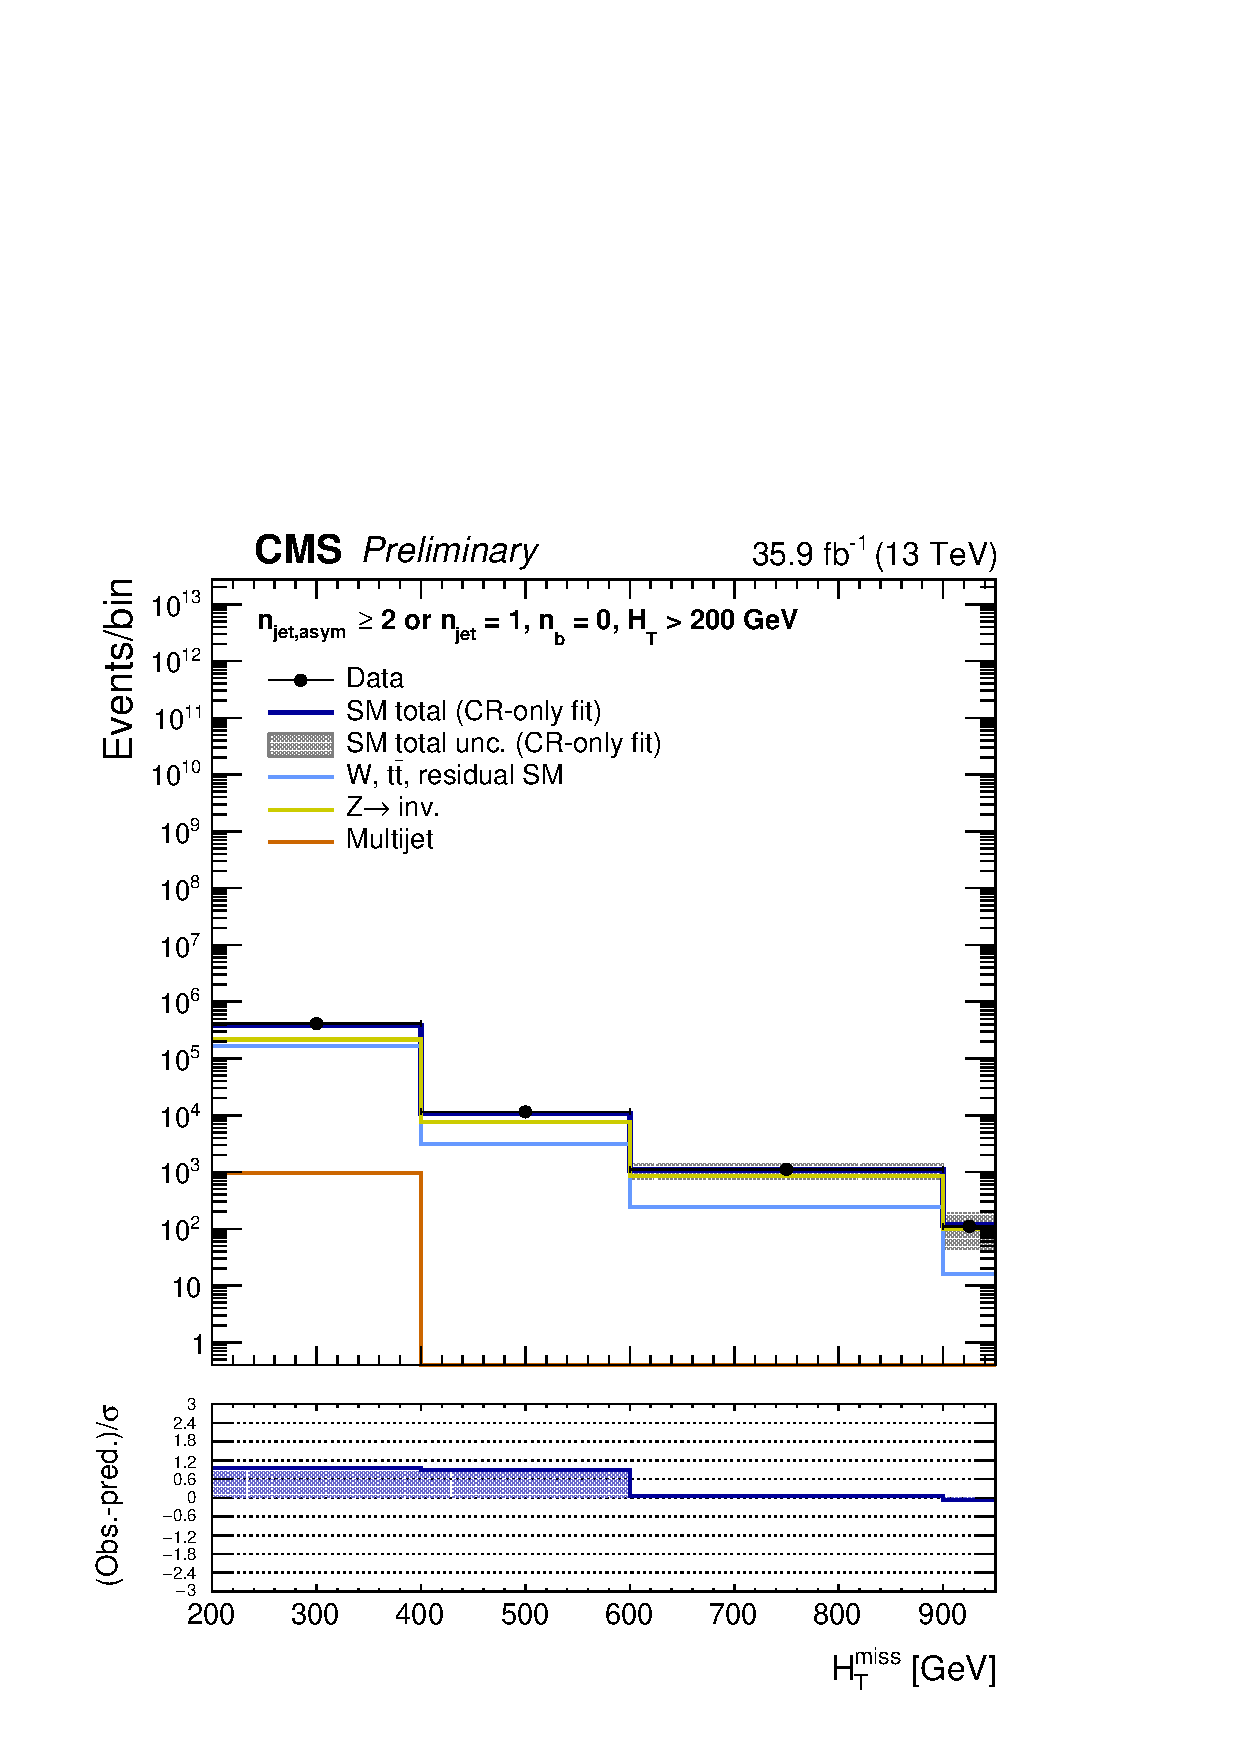
\includegraphics[width=0.49\linewidth]{figures/results/36invfb_preapproval/aggregated/postFitShapeCR/mhtShape_eq0b_ge1j2a_200_Inf_crfit.pdf} ~
  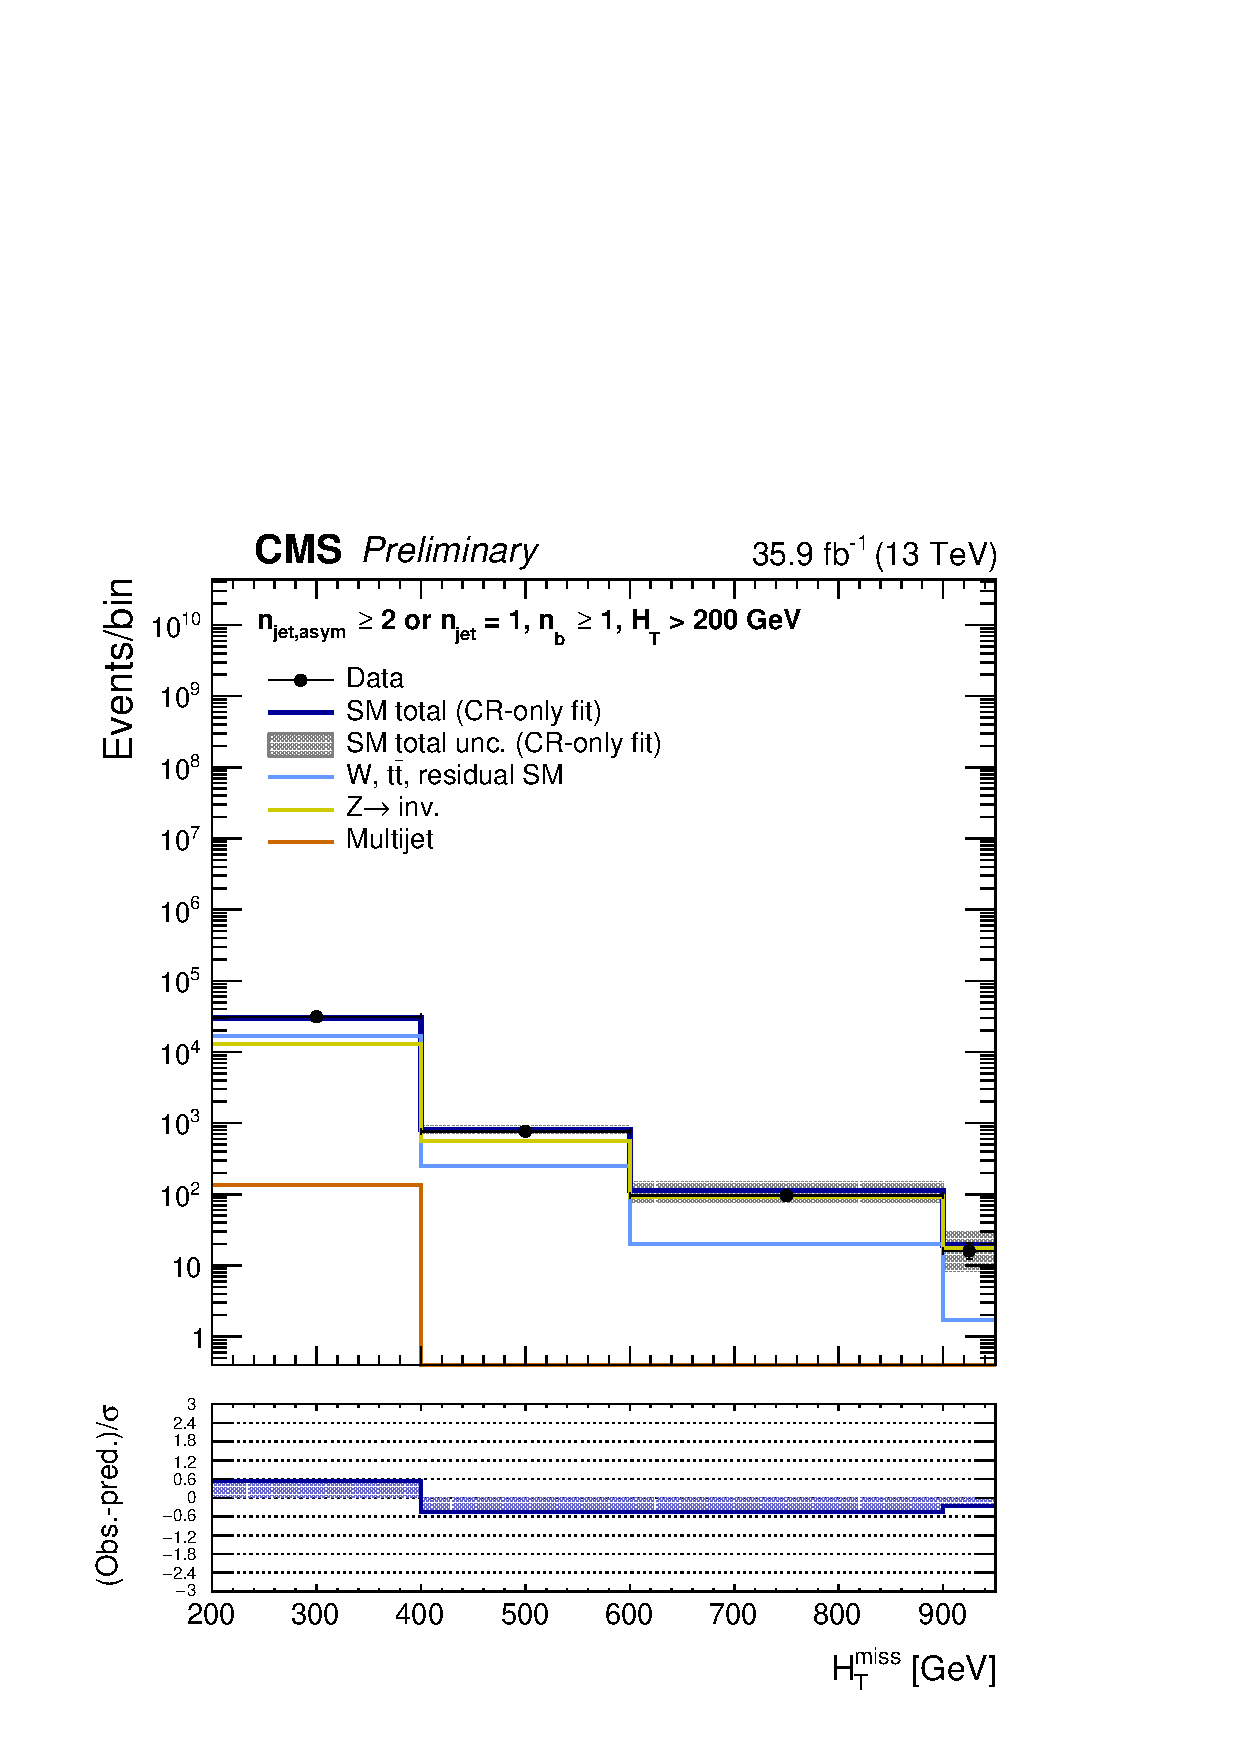
\includegraphics[width=0.49\linewidth]{figures/results/36invfb_preapproval/aggregated/postFitShapeCR/mhtShape_ge1b_ge1j2a_200_Inf_crfit.pdf} 
  \label{fig:aggregated_results1}
\end{figure}

\clearpage
\begin{figure}[h!]
  \centering
  \caption{
    \customcaption{``low \njet''}{$2 \leq \njet \leq 3$}{$\scalht > 200\GeV$}{$0 \leq \nb \leq 1$}{$\nb \geq 2$}
  }
  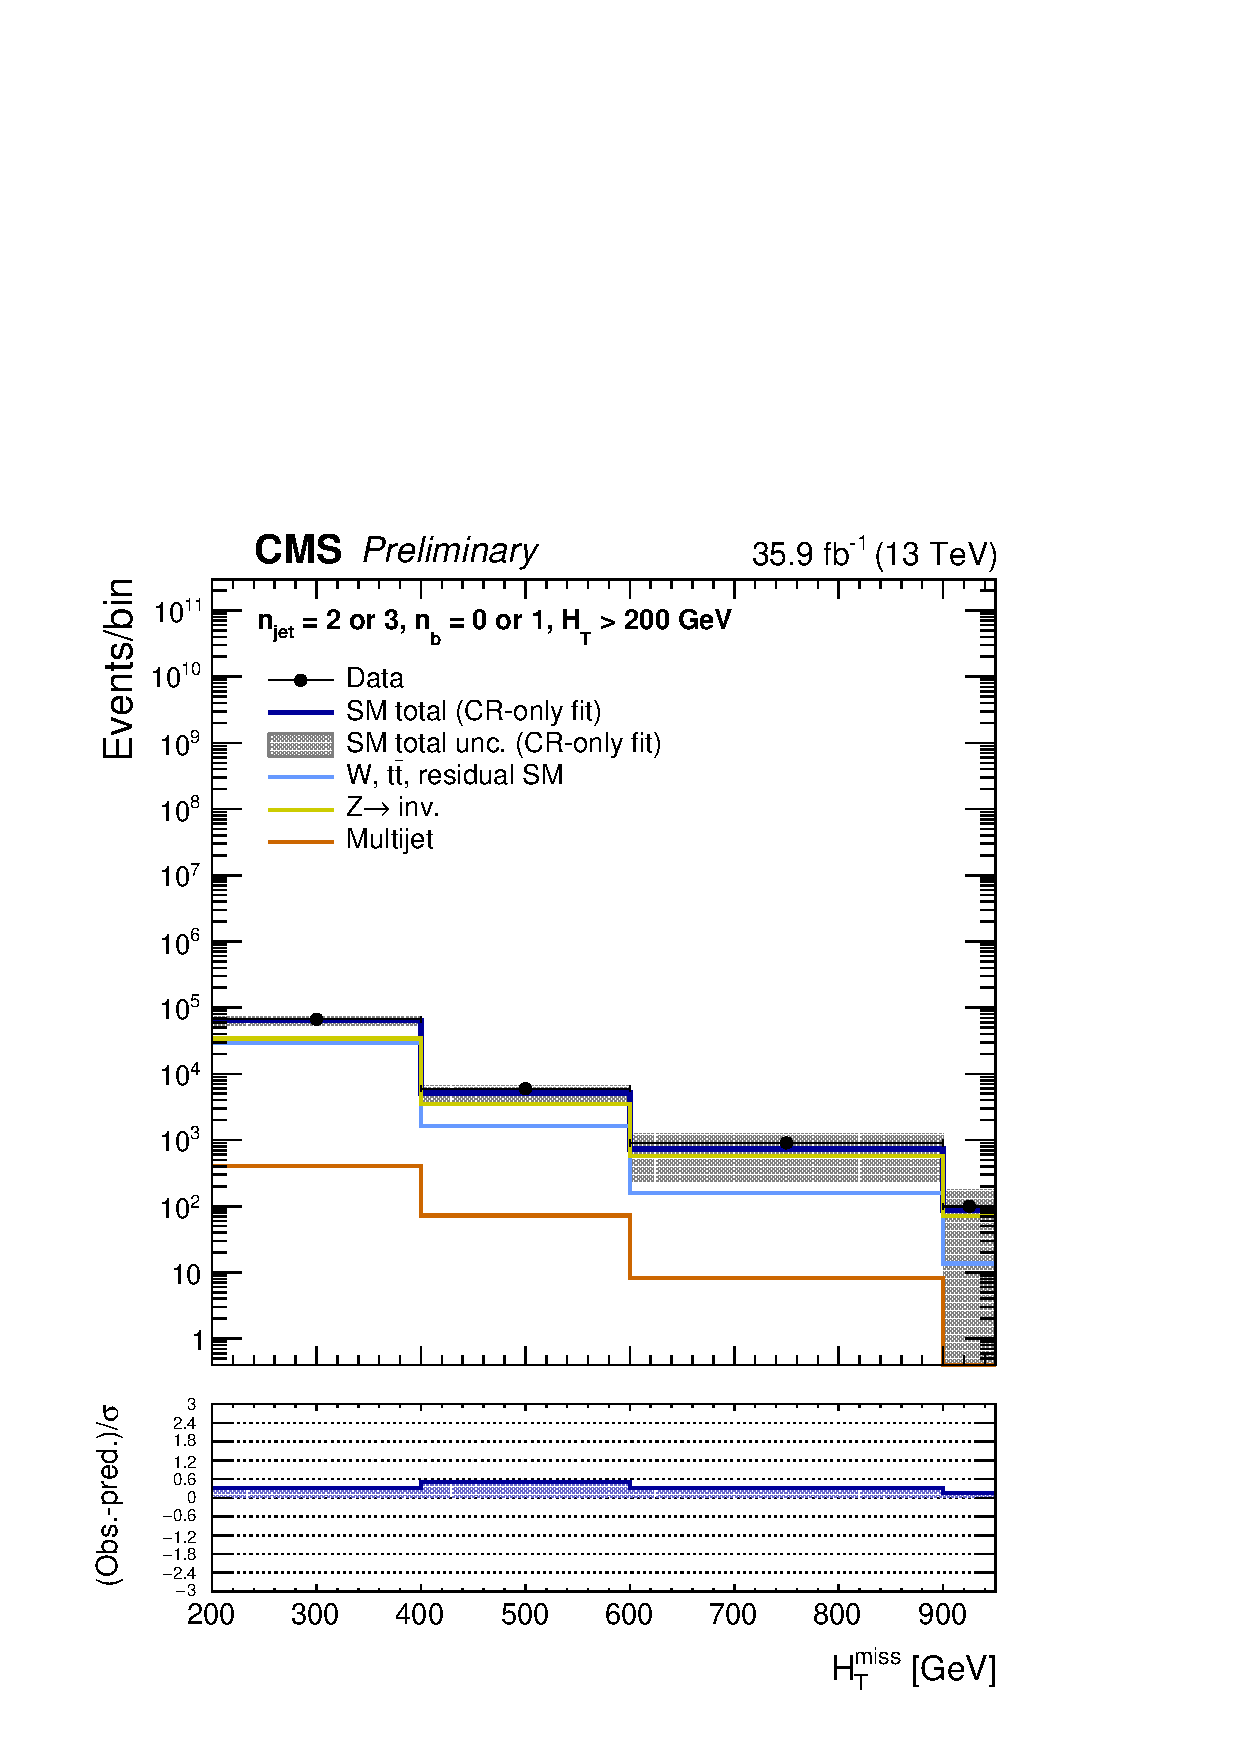
\includegraphics[width=0.49\linewidth]{figures/results/36invfb_preapproval/aggregated/postFitShapeCR/mhtShape_eq01b_eq23j_200_Inf_crfit.pdf} ~
  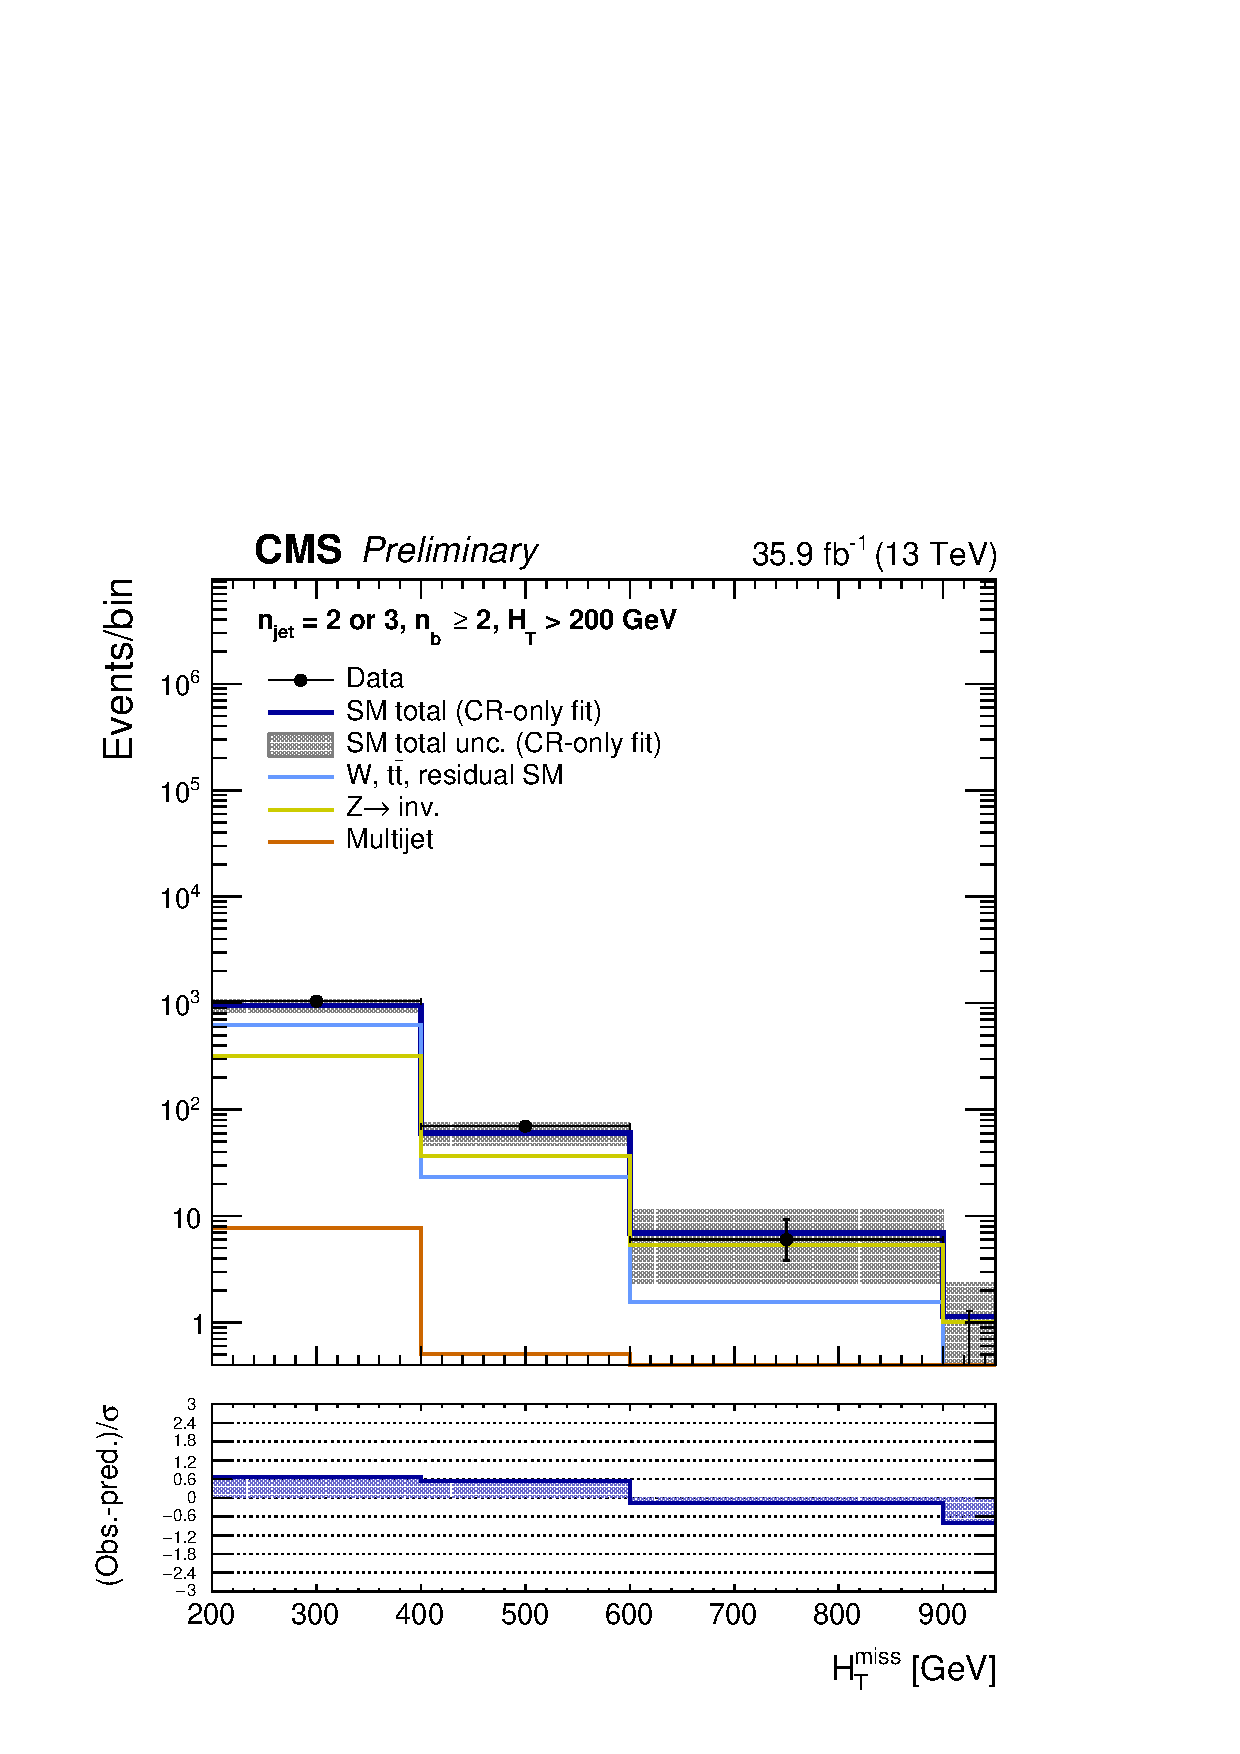
\includegraphics[width=0.49\linewidth]{figures/results/36invfb_preapproval/aggregated/postFitShapeCR/mhtShape_ge2b_eq23j_200_Inf_crfit.pdf} 
  \label{fig:aggregated_results2}
\end{figure}

\clearpage
\begin{figure}[h!]
  \centering
  \caption{
    \customcaption{``medium \njet''}{$4 \leq \njet \leq 5$}{$\scalht > 400\GeV$}{$0 \leq \nb \leq 1$}{$\nb \geq 2$}
  }
  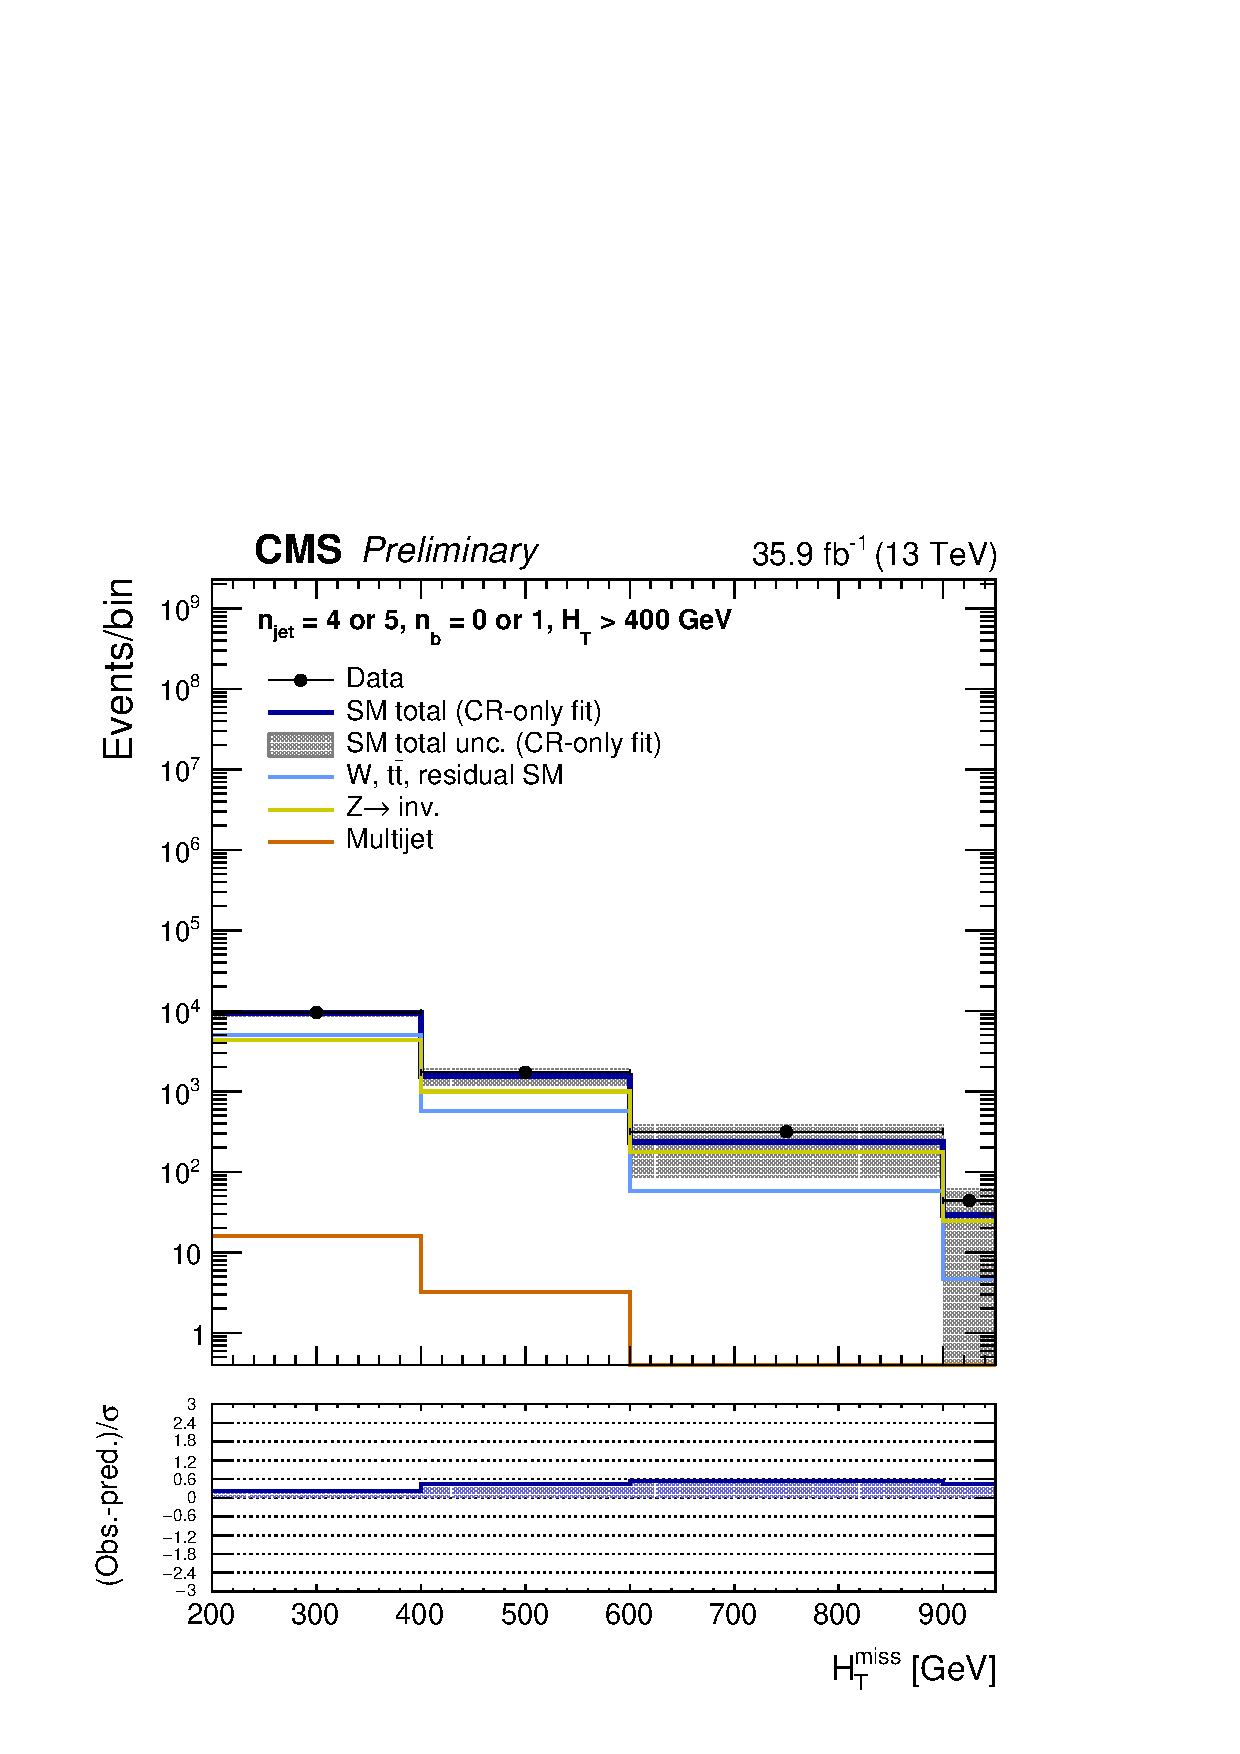
\includegraphics[width=0.49\linewidth]{figures/results/36invfb_preapproval/aggregated/postFitShapeCR/mhtShape_eq01b_eq45j_400_Inf_crfit.pdf} ~
  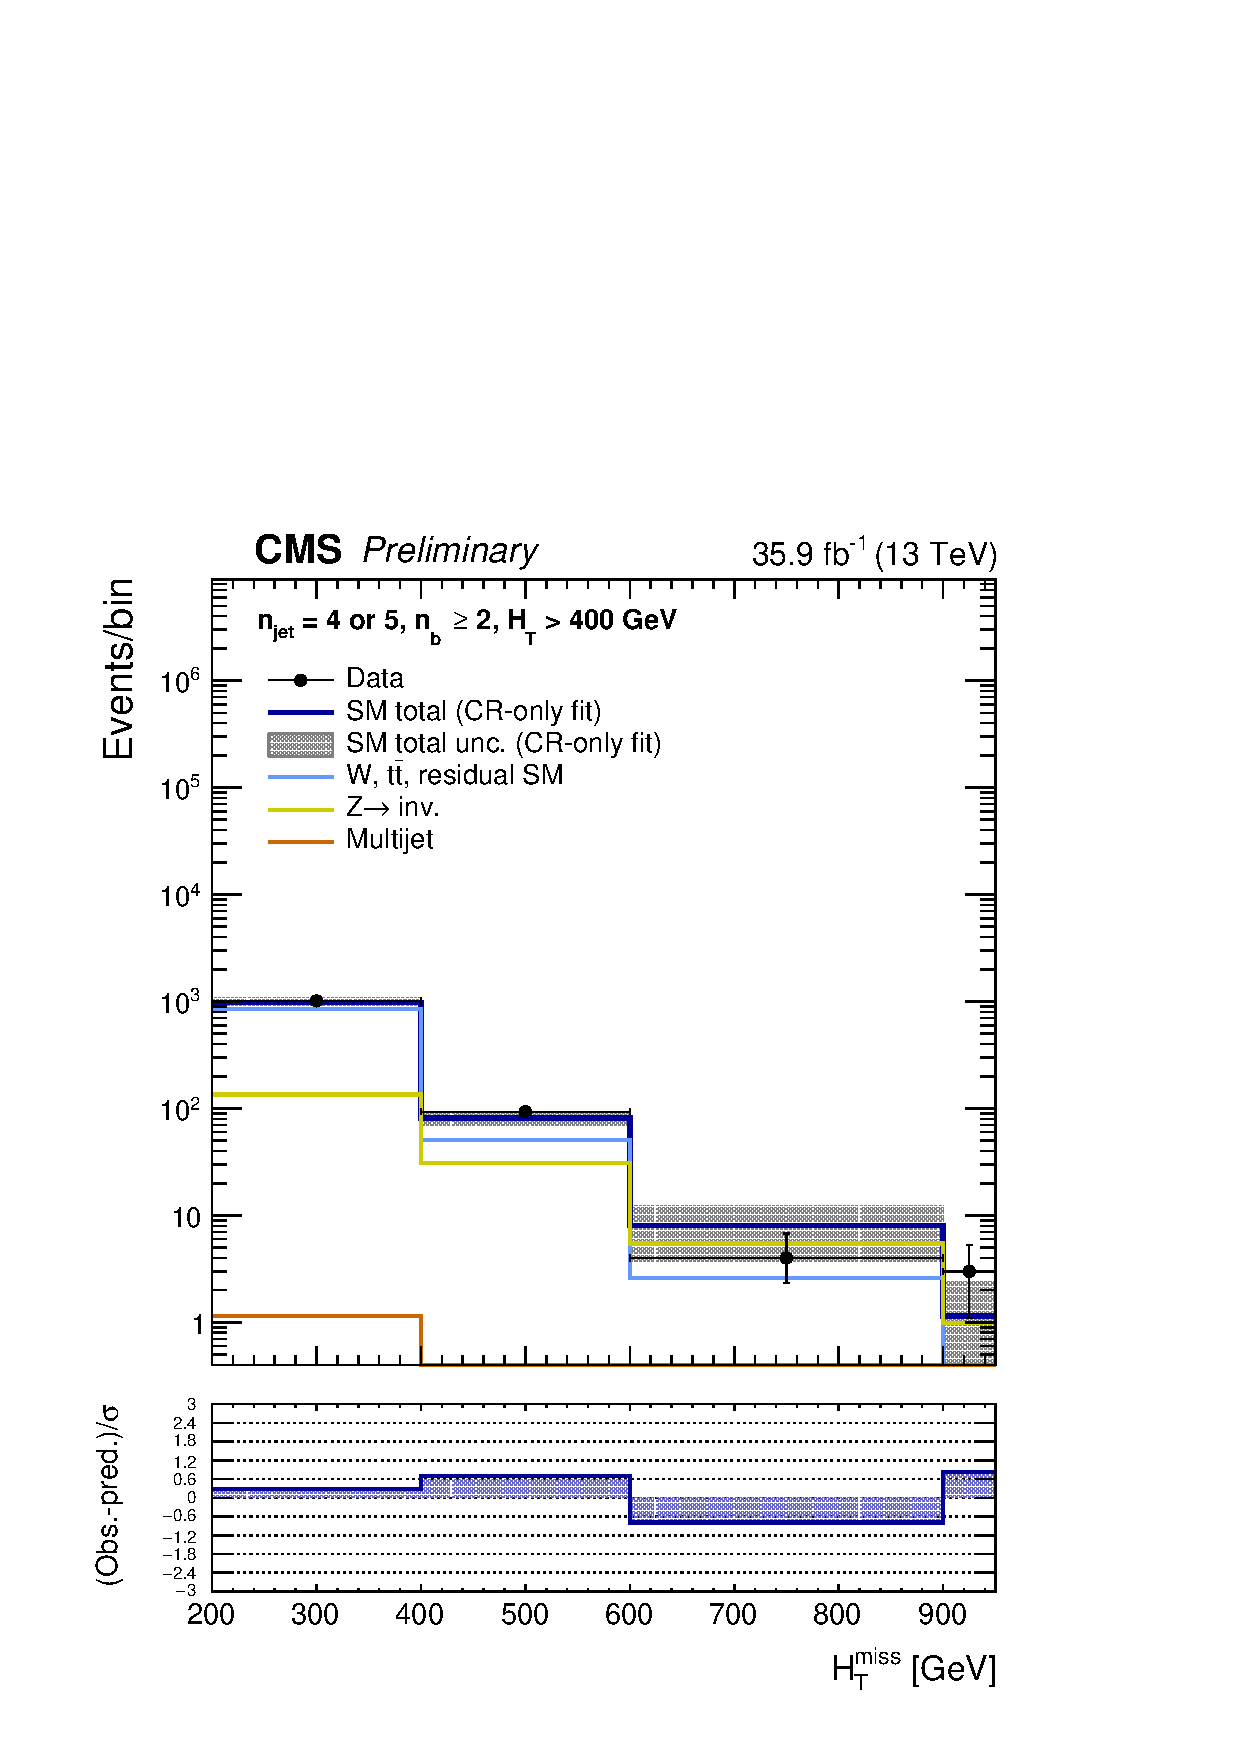
\includegraphics[width=0.49\linewidth]{figures/results/36invfb_preapproval/aggregated/postFitShapeCR/mhtShape_ge2b_eq45j_400_Inf_crfit.pdf} 
  \label{fig:aggregated_results3}
\end{figure}

\clearpage
\begin{figure}[h!]
  \centering
    \caption{
      \customcaption{``high \njet''}{$\njet \geq 6$}{$\scalht > 400\GeV$}{$0 \leq \nb \leq 1$}{$\nb \geq 2$}
    }
  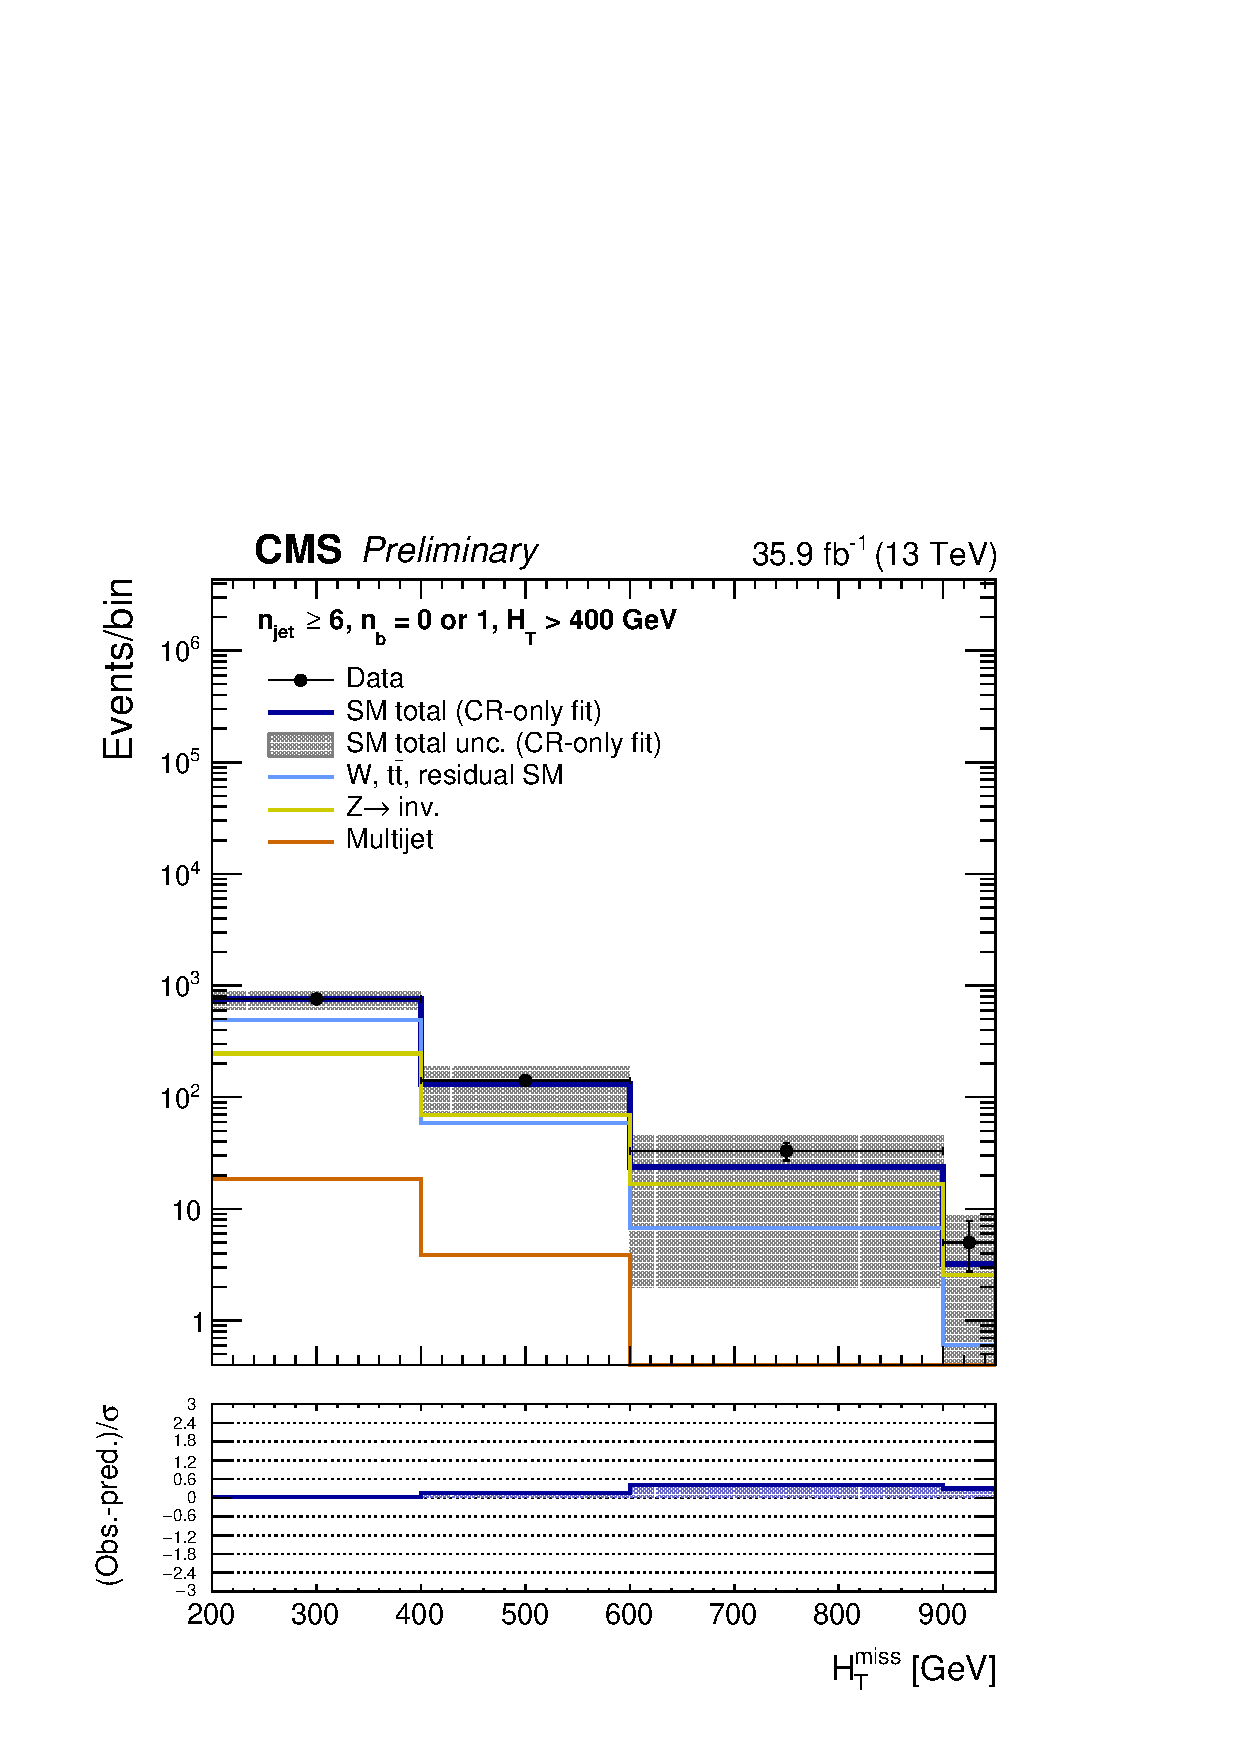
\includegraphics[width=0.49\linewidth]{figures/results/36invfb_preapproval/aggregated/postFitShapeCR/mhtShape_eq01b_ge6j_400_Inf_crfit.pdf} ~
  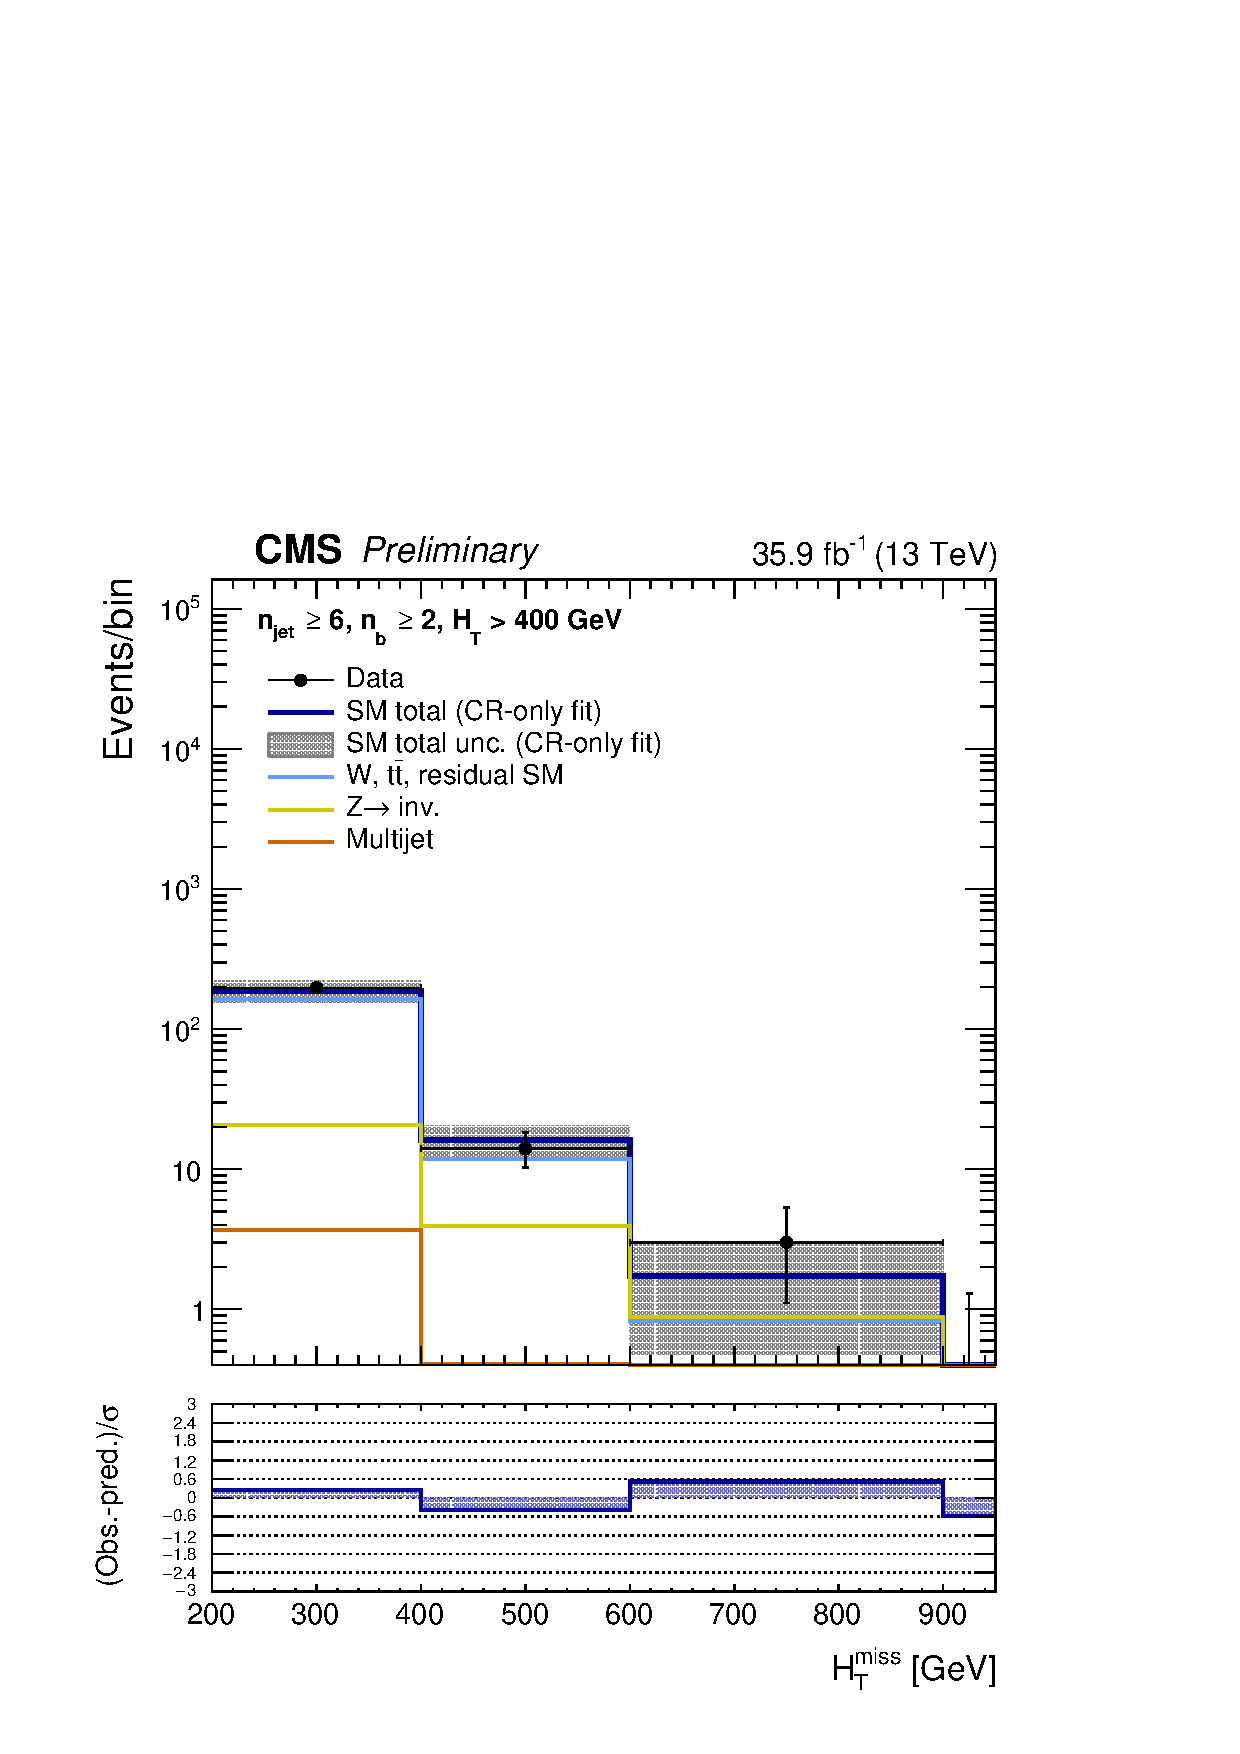
\includegraphics[width=0.49\linewidth]{figures/results/36invfb_preapproval/aggregated/postFitShapeCR/mhtShape_ge2b_ge6j_400_Inf_crfit.pdf}
  \label{fig:aggregated_results4}
\end{figure}

\clearpage
\begin{figure}[h!]
  \centering
  \caption{Covariance matrix for the background
    predictions based on aggregated signal regions} 
  }
  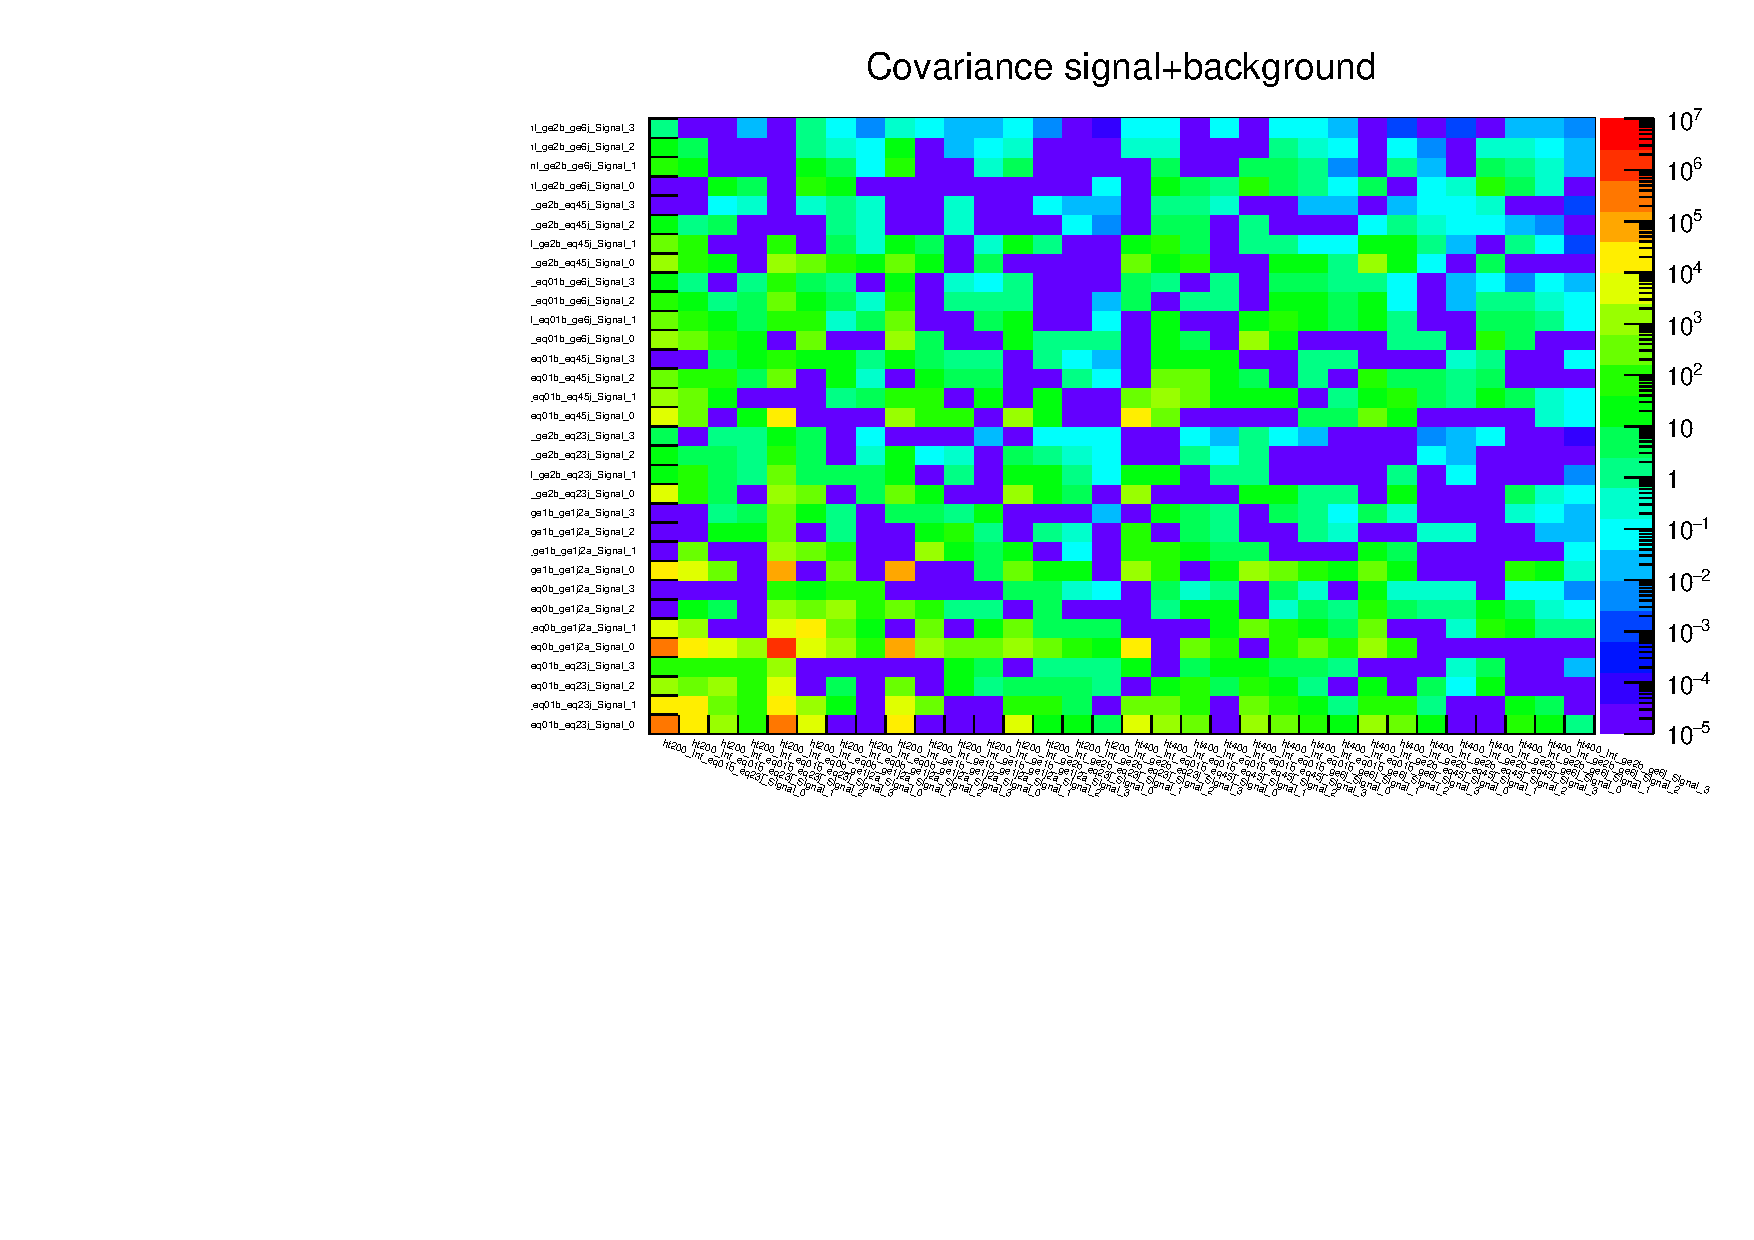
\includegraphics[width=0.8\linewidth]{figures/results/36invfb_preapproval/aggregated/covariance}
  \label{fig:covar}
\end{figure}

\clearpage
\begin{figure}[h!]
  \centering
  \caption{Correlation matrix for the background
    predictions based on aggregated signal regions} 
  }
  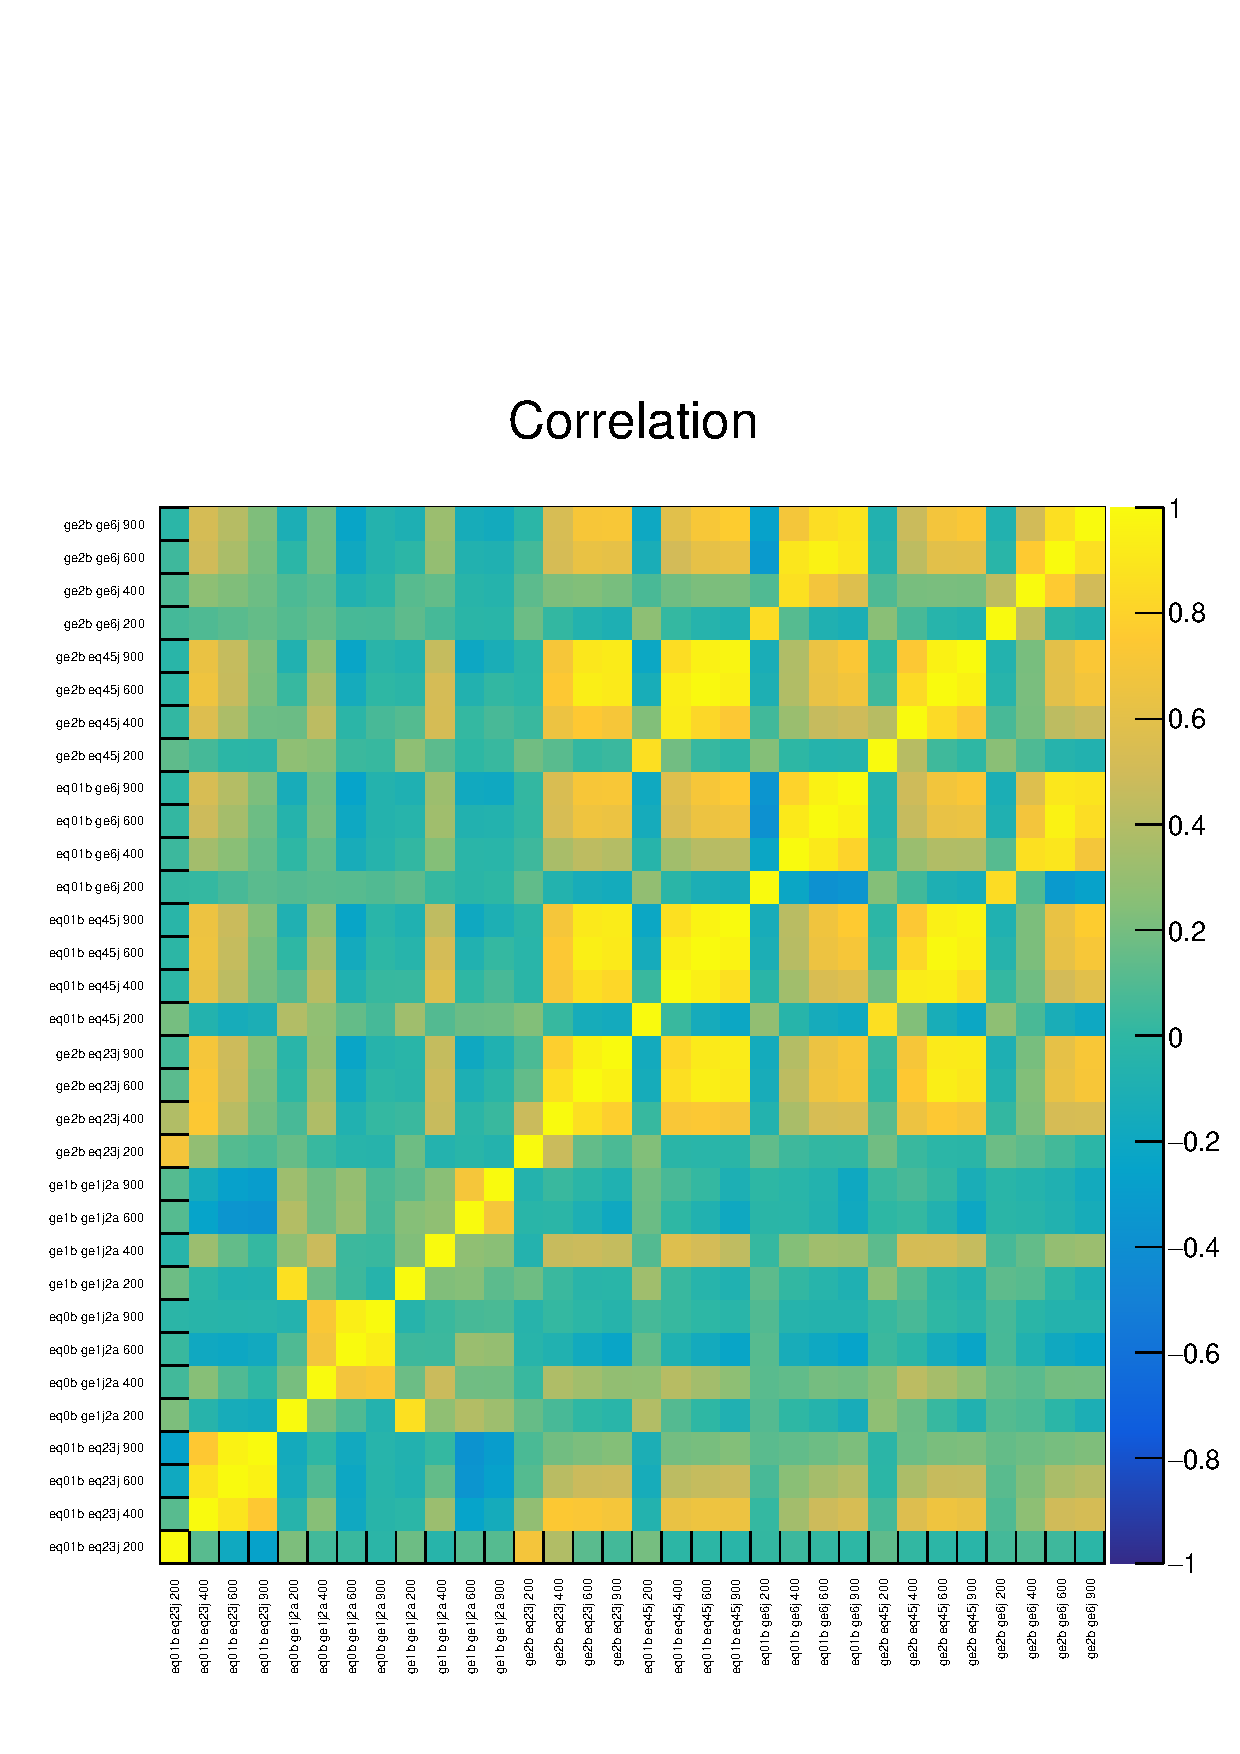
\includegraphics[width=0.8\linewidth]{figures/results/36invfb_preapproval/aggregated/correlation}
  \label{fig:corr}
\end{figure}
